%!TEX root = ../template.tex
%%%%%%%%%%%%%%%%%%%%%%%%%%%%%%%%%%%%%%%%%%%%%%%%%%%%%%%%%%%%%%%%%%%%
%% chapter4.tex
%% NOVA thesis document file
%%
%% Chapter with the system architecture
%%%%%%%%%%%%%%%%%%%%%%%%%%%%%%%%%%%%%%%%%%%%%%%%%%%%%%%%%%%%%%%%%%%%
\chapter{System Architecture}
\label{cha:system_architecture}

\begin{quotation}
\begin{flushright}
\itshape
«missing quote...»\\
\textbf{- Author}
\end{flushright}
\end{quotation}

On this chapter, the complete system architecture will be presented, starting by describing the system's requirements based on the thesis goals. It will be followed by an introduction to the main system components, and end with a detailed description of the system's architectural layers.

% ==========================
% = System requirements =
% ==========================

\section{System Requirements}
\label{sec:system_architecture_requirements}

In order to properly develop the present work, the system's requirements must be considered.

In general terms, this system must have into consideration requirements associated with the particular needs of bioprinting like resolution, printing speed, and bioink compatibility. It should also consider the particularities of how to position the print head within the wound area. Depending on the degree of autonomy, it must also be considered how the wounds will be detected and referenced within the positioning system. Physical constraints like dimensions and weight are also important. Lastly, but also vital, are the safety requirements. Some of these requirements are considered needed improvements of bioprinting systems, or are related to them \cite{Ozbolat2017_evaluation_bioprinter_tech}. A more complete list of the main requirements for this system, by category, is presented on figure \ref{fig:system_requirements}. Each requirement will be described in more detail.

\begin{figure}[htbp]
	\centering
	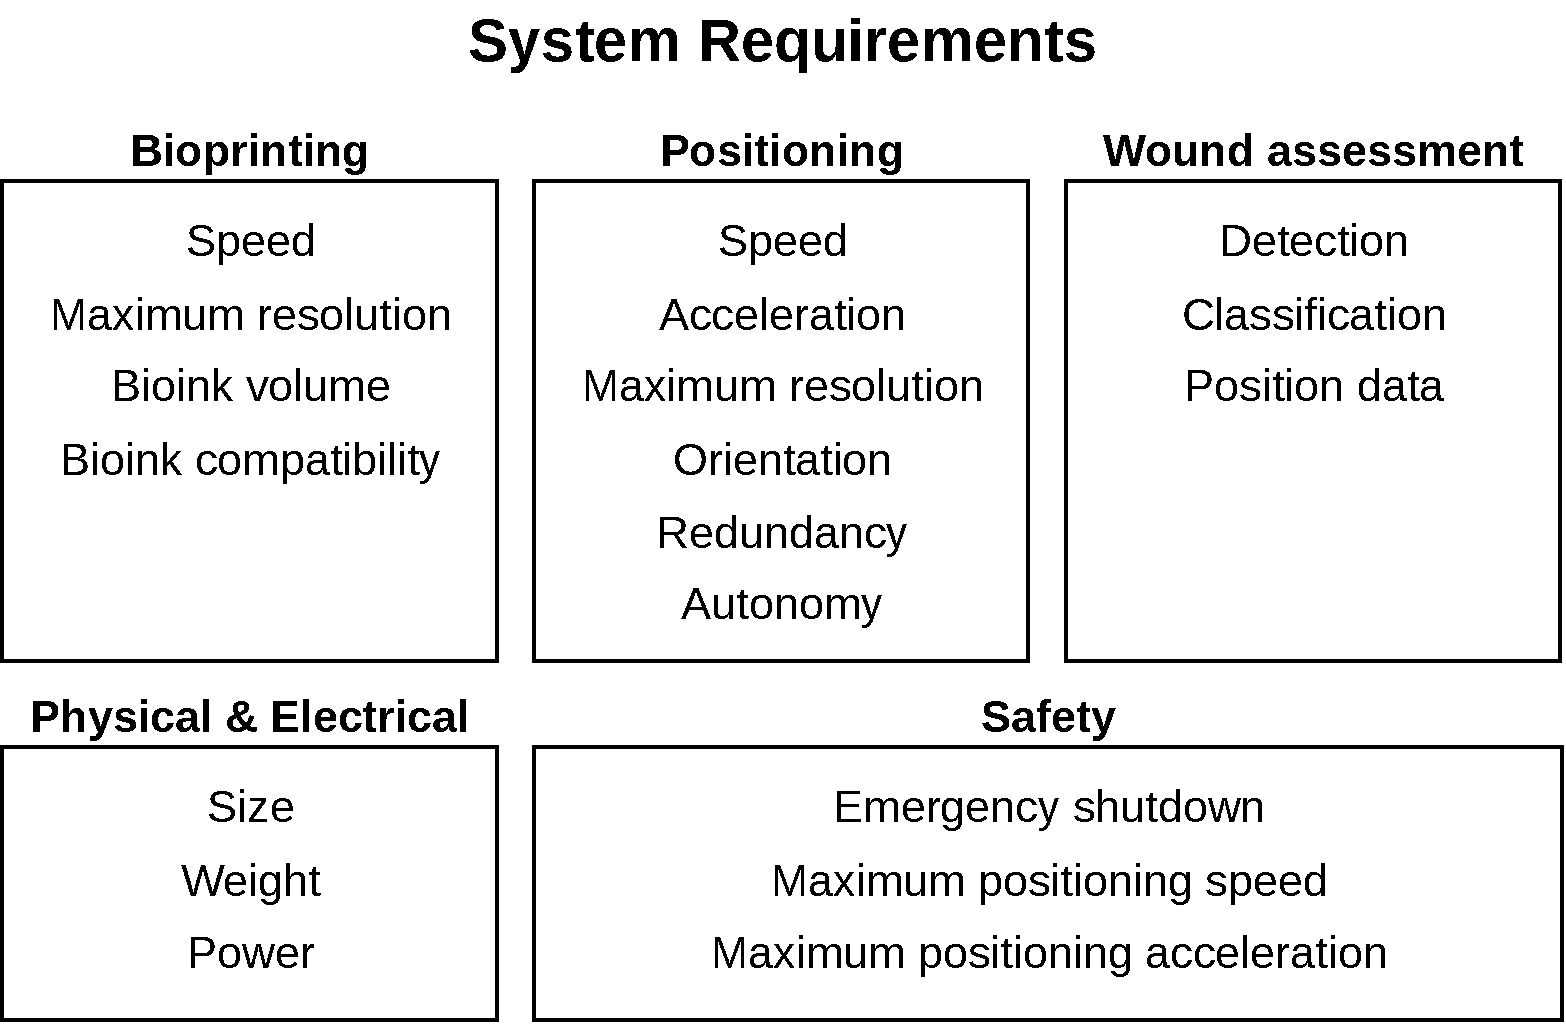
\includegraphics[width=0.7\textwidth]{system_requirements}
	\caption{System requirements.}
	\label{fig:system_requirements}
\end{figure}

\subsection{Bioprinting Speed}
\label{subsec:system_architecture_requirements_bioprinting_speed}

In order for the system to provide real clinical value it must allow the bioprinting procedure to execute at a certain speed. Because the printing will be in situ, the skin construct cannot be previously printed for later use. In order to be practical to the clinicians, the bioprinting system should execute the printing within the time frame of a wound dressing procedure, or preferably in less time.

Other reasons why the printing speed may be important concern the bioink characteristics like gelation time and cell viability. The gelation time, is the time needed for the biokink to solidify. Sometimes, to reduce this time, different strategies are followed, like UV curing, depending on the bioink. The cell viability is conditioned by the speed because of induced shear stress added when trying to squeeze the cell-laden bioink out of the nozzle. 

This requirement will inevitably constrain the choice of the printing method. The choice must take into account practical operational needs and bioprinting technical needs.

Table \ref{tab:system_architecture_requirements_bioprinting_methods_comparison} presents the average speeds of the various printing methods. The proposed system should at least be able to replicate the printing speeds according to the printing method chosen.

% subsection system_architecture_requirements_bioprinting_speed

\subsection{Bioprinting Maximum Resolution}
\label{subsec:system_architecture_requirements_bioprinting_max_resolution}

The printing resolution will condition the detail of the structures obtained, the printing speed and the resolution of the positioning system. It depends on the printing method and bioink characteristics.

Regarding the method used, the values "5, 50 and 100 \si{\micro\meter} are typically obtained by \gls{lbb}, \gls{dbb} and \gls{ebb}, respectively" \cite{Datta2018_essential_steps_bioprinting}. Table \ref{tab:system_architecture_requirements_bioprinting_methods_comparison} presents a general comparison of the resolution of the various methods.

% subsection system_architecture_requirements_bioprinting_max_resolution

\subsection{Bioink Volume}
\label{subsec:system_architecture_requirements_bioprinting_bioink_volume}

This criteria is very important on our particular application. The print head volume will define the amount of bioink that can be used in one go. Because we can deal with large wounds, it is important to have a good volume. If the volume is small, it may require several refills, which would affect considerably the printing time. However, there should be an upper limit based on print head weight and size, and common wound sizes.\\

According to \citeauthor{Redlarski2016_bsa_formulae_alarming_ambiguity} \cite{Redlarski2016_bsa_formulae_alarming_ambiguity}, even with the existence of a large number of formulas for calculating the \gls{bsa}, DuBois's formula \cite{DuBOIS1916_formula} is still considered the standard. Using that formula (\ref{eq:dubois_formula}), we will try to estimate a proper volume for the printing head bioink container.

\begin{equation}
\label{eq:dubois_formula}
    BSA = 0.007184 \times W^{0.425} \times H^{0.725}
\end{equation}

The formula calculates the \gls{bsa} in \si{\meter\squared} and depends on weight ($W$) in kilograms and height ($H$) in centimetres. Assuming an average height of 180 cm and weight of 80 kg, the DuBois formula returns a \gls{bsa} of 1.996 \si{\meter\squared}. Considering an average wound thickness of 2 \si{\milli\meter}, calculations of wound volume were done and are presented on table \ref{tab:system_architecture_requirements_wound_volumes}.

\begin{table}[ht]
	\caption{Wound filling volumes for various \%\gls{tbsa} values, calculated with the DuBois's formula for an average height of 180 cm, weight of 80 kg and wound depth of 2 \si{\milli\meter}. For calculations, the \gls{bsa} value was rounded to whole number.}
	\label{tab:system_architecture_requirements_wound_volumes}
\centering
\begin{tabular}{lc}
	\toprule
	\textbf{\%\gls{tbsa}} & \textbf{Wound volume (\si{\milli\liter})}\\
	\midrule

    1\% & 40 \\
    2\% & 80 \\
    5\% & 200 \\
    10\% & 400 \\
    20\% & 800 \\
    30\% & 1200 \\
    50\% & 2000 \\
    \bottomrule
\end{tabular}
\end{table}

For the system to be remain lightweight, the print head should not be heavier than 0.5 \si{\kilo\gram}. Assuming the density of water for the bioink, a volume of 400 \si{\milli\liter} would weight 0.4 \si{\kilo\gram}. Since the print head is more than the bioink volume and container, we should consider some extra weight. Having all that into consideration, a bioink volume of 200 \si{\milli\liter} seems like a good goal. It reduces weight and it still allows us to handle a 5\% \gls{tbsa}.

% subsection system_architecture_requirements_bioprinting_bioink_volume

\subsection{Bioink Compatibility}
\label{subsec:system_architecture_requirements_bioprinting_bioink_compatibility}

Bioinks for skin bioprinting are generally composed by two components. One is a natural or artificial polymeric hydrogel that forms a scaffold meant to replicate the \gls{ecm}. The other is the group of cells or biomolecules that will effectively develop the tissue being printed [\cite{Vijayavenkataraman2016_stateart_modelling_materials_processing, Yan2018_3dprinting_skin_tissue_preprocessing_final_eval, Tarassoli2018_skin_tissue_engineering_3dbioprinting_evolving_research_field}].

Besides hydrogels, there are other bioink materials like \gls{decm}, microcarriers, and cell aggregates. The selection of any of this materials is conditioned by the printing method chosen, because they are not all compatible.

According with \citeauthor{Hospodiuk2017_bioink_comprehensive_review_bioprintable_materials}\cite{Hospodiuk2017_bioink_comprehensive_review_bioprintable_materials} extrusion-based bioprinting is the most flexible printing method regarding bioink compatibility. It facilitates the bioprinting of "hydrogels, cell aggregates (in spheroid, strand and cell pellet form), \gls{decm} components and microcarriers in bulk hydrogels". \gls{dbb} and \gls{lbb} methods only support bioprinting hydrogels.

\begin{table}[ht]
	\caption{Comparison of various bioprinting methods \cite{Vijayavenkataraman2018_bioprinting_tissues_organs_regen_med}.}
	\label{tab:system_architecture_requirements_bioprinting_methods_comparison}
\centering
\begin{adjustbox}{width=1.2\textwidth,center=\textwidth}
\begin{tabular}{lccccccc}
	\toprule
	\textbf{Properties} & \textbf{Laser-based} & \textbf{Inkjet} & \textbf{EHD-jetting} & \textbf{Acoustic} & \textbf{Microvalve} & \textbf{Extrusion-based} & \textbf{Stereolithography}\\
    & \textbf{bioprinting} & \textbf{bioprinting} & \textbf{based} & \textbf{bioprinting} & \textbf{bioprinting} & \textbf{bioprinting} & \textbf{bioprinting}\\
    & & & \textbf{bioprinting} & & & &\\
	\midrule

Bioink viscosity & 1–300 mPa·s & 3–12 mPa·s & 1–1000 mPa·s & - & 1–200 mPa·s & ~600 kPa·s & ~5 Pa·s \\

Cell density & $10^8$ cells/ml & $10^6$ cells/ml & $10^6$ cells/ml & $10^6$ cells/ml & $10^6$ cells/ml & $10^8$ cells/ml & $>10^6$ cells/ml\\

Speed & 200–1600 mm/s & 10,000 droplets/s & 10–500 mm/s & 10,000 droplets/s & 1000 droplets/s & 10–50 \si{\micro\meter}/s & High\\

Resolution & 50 \si{\micro\meter} & 50 \si{\micro\meter} & 100 nm & 37 \si{\micro\meter} & - & 100 \si{\micro\meter} & 200 nm - 6 \si{\micro\meter}\\

Accuracy & High & Medium & Low & Medium & Medium & Low & High\\

Cell viability & >95\% & >80\% & >80\% & >90\% & >80\% & 40-95\% & 25-85\%\\

Structural integrity & Low & Low & High & Low & Low-Medium & High & Medium-High\\

Scalability & Low & High & High & Medium & High & High & Medium-High\\

Cost & High & Low & High & Medium-High & Medium & Low-Medium & Medium \\
    \bottomrule
\end{tabular}
\end{adjustbox} 
\end{table}


% subsection system_architecture_requirements_bioprinting_bioink_compatibility

\subsection{Positioning Speed}
\label{subsec:system_architecture_requirements_positioning_speed}

The speed of the positioning system must match the needs of the printing speed. Its maximum speed must exceed the printing speed, so that it can follow the printing process on the full range of speeds. Also, since the shape of the wound can be non-planar, all the axis should be able to reach speeds greater that the maximum printing speed.

When choosing the positioning system the printing method must be considered to define the speed limits. For example, if the printing method is extrusion-based, then the positioning system must reach speeds greater than 50 \si{\micro\meter\per\second}, according to table \ref{tab:system_architecture_requirements_bioprinting_methods_comparison}.

% subsection system_architecture_requirements_positioning_speed

\subsection{Positioning Acceleration}
\label{subsec:system_architecture_requirements_positioning_acceleration}

The positioning acceleration is important to guarantee that the robot can reduce its speed to zero very fast. It can also be important depending on the printing trajectories. A sudden change in direction will need a high acceleration. The positioning system must allow for high accelerations even if they are not always needed.

% subsection system_architecture_requirements_positioning_acceleration

\subsection{Positioning Maximum Resolution}
\label{subsec:system_architecture_requirements_positioning_max_resolution}

The maximum resolution of the positioning system is the minimum repeatable step size. This will define the precision of the system. It is very important that this value is lower than the bioprinting resolution, by at least one order of magnitude. In case this is not possible, the printing method must be adapted to accommodate for this limitation and still be effective.

Gantry systems can have very high resolutions. That is one of the reasons they are so often used in 3D printing and bioprinting. Other robotic manipulators on the other hand, can have many degrees of freedom, but typically lose resolution because of that.

% subsection system_architecture_requirements_positioning_max_resolution

\subsection{Positioning Orientation}
\label{subsec:system_architecture_requirements_positioning_orientation}

For this specific application, the print head orientation is very relevant. We have to consider a system that must be able to print on a wound that is located anywhere in the body. To be more practical it would also be ideal for the system to move according to the patient position instead of the other way around. Because of this, the print head may need to work in various non vertical orientations.

Gantry systems have the limitation of having a fixed orientation. Robotic manipulators with more degrees of freedom can have partial or full orientation freedom.

% subsection system_architecture_requirements_positioning_orientation

\subsection{Positioning Redundancy}
\label{subsec:system_architecture_requirements_positioning_redundancy}

Another important aspect of positioning is redundancy. This means having extra degrees of freedom to handle obstacles, for example. Having extra \gls{dof} for a specific task allows the system to position the print head on one place with different configurations. This facilitates the system's adaptation to the patient versus the patient adapting to the system.

% subsection system_architecture_requirements_positioning_redundancy

\subsection{Positioning Autonomy}
\label{subsec:system_architecture_requirements_positioning_autonomy}

The degree of autonomy of the positioning system must also be considered. The system may be fully autonomous using sensing data to detect the wound, position itself along it, and execute the printing. But it can also work semi-autonomously, where the clinician manipulates the system as a tool and controls the printing directly. In this case, the positioning system only provides some extra control on the procedure.

% subsection system_architecture_requirements_positioning_autonomy

\subsection{Wound Assessment Detection}
\label{subsec:system_architecture_requirements_wound_assessment_detection}

Since the goal is to print directly on a wound, the system must be able to detect the wound. This detection can be operator dependent, i.e., the operator guides the positioning system towards the wound area. Another possibility is to use a sensing system to detect the wound and guide the positioning system. It is somewhat related to positioning autonomy.

The are several possibilities for this wound detection as was shown on chapter \ref{cha:literature_review}.

% subsection system_architecture_requirements_wound_assessment_detection

\subsection{Wound Assessment Classification}
\label{subsec:system_architecture_requirements_wound_assessment_classification}

Wound classification is the action of extracting meaningful data after detection. Some important data to support the autonomy of the printing process is measuring the wound area and perimeter. Other important parameters may be the depth and profile.

The wound area is important to calculate the amount of bioink needed for the print. It also can help the clinicians in assessing the \gls{tbsa}. 

% subsection system_architecture_requirements_wound_assessment_classification

\subsection{Wound Assessment Position Data}
\label{subsec:system_architecture_requirements_wound_assessment_position_sharing}

After wound detection by a sensing system, the wound position must be shared with the positioning system for the printing to occur on the right place. The data sharing process and the data itself must be considered. It will depend on the sensing system, but at least a reference transformation between the sensing system and the positioning system must exist.

% subsection system_architecture_requirements_wound_assessment_position_sharing

\subsection{Physical Size}
\label{subsec:system_architecture_requirements_physical_size}

As in all physical products, the size is always something to consider. The system will be installed on a operating room or a patient room, which are not huge and many times already crowded with other tools and machines. So, in this case, the whole system should not be too big. It should occupy the least space possible, but still have enough range to reach a large portion of the patient's body.

% subsection system_architecture_requirements_physical_size

\subsection{Physical Weight}
\label{subsec:system_architecture_requirements_physical_mass}

The system's mass is also important. It should weight as less as possible. One specific reason for this is for safety. Since the positioning system maybe working autonomously close to the patient, it is vital to have a reduced mass in case of contact. 

Another reason is for manipulation. If the system is to be manipulated directly by an operator for the bioprinting procedure, it facilitates if it is low weight. The system must help the clinicians, not introduce more hurdles.

The mass also interferes with the degree of portability of the system. It if it is light, it can be moved between difference spaces easily. This facilitates the process of taking the system to where it is needed.

% subsection system_architecture_requirements_physical_mass

\subsection{Electrical Power}
\label{subsec:system_architecture_requirements_physical_power}

If the system can use the normal mains power from 100 to 240 VAC to operate, it does not need a special installation. This will help cut down costs and ease the installation. If the system was three-phase, for example, the electrical system on the room would most certainly need to be updated.

% subsection system_architecture_requirements_physical_power

\subsection{Safety Emergency Shutdown}
\label{subsec:system_architecture_requirements_safety_emergency_shutdown}

For safety considerations, an emergency shutdown must be considered. The system will be in almost direct contact with the patient during printing. If something goes wrong, there must exist a way to turn off the system to prevent any or further injuries to the patient/operator.

% subsection system_architecture_requirements_safety_emergency_shutdown

\subsection{Safety Maximum Positioning Speed}
\label{subsec:system_architecture_requirements_safety_max_positioning_speed}

Although having a fast positioning system is good, a maximum limit must exist that minimises the chance of injury if an accidental contact between a person and the system occurs. The system should allow to set a speed limit below its physical limits.

% subsection system_architecture_requirements_safety_max_positioning_speed

\subsection{Safety Maximum Positioning Acceleration}
\label{subsec:system_architecture_requirements_safety_max_positioning_acceleration}

Regarding the acceleration, there must be a maximum limit, as with speed, to prevent any injuries or minimise the consequences of one. Since a human and a robot will be working on the same space, any safety measure available must be considered. The system should allow to set an acceleration limit below its physical limits.

% subsection system_architecture_requirements_safety_max_positioning_acceleration

% section system_architecture_requirements

% ==========================
% = System Components =
% ==========================

\section{System Components}
\label{sec:system_architecture_components}

Based on the system requirements previously mentioned, the system suggested is composed by three main components (Fig. \ref{fig:system_architecture_components}): (a) a robotic system composed by a robotic manipulator that is responsible for positioning the print head in space; (b) a vision system responsible for wound assessment; and (c) a bioprinting system composed by an extrusion-based print head.

\begin{figure}[htbp]
	\centering
	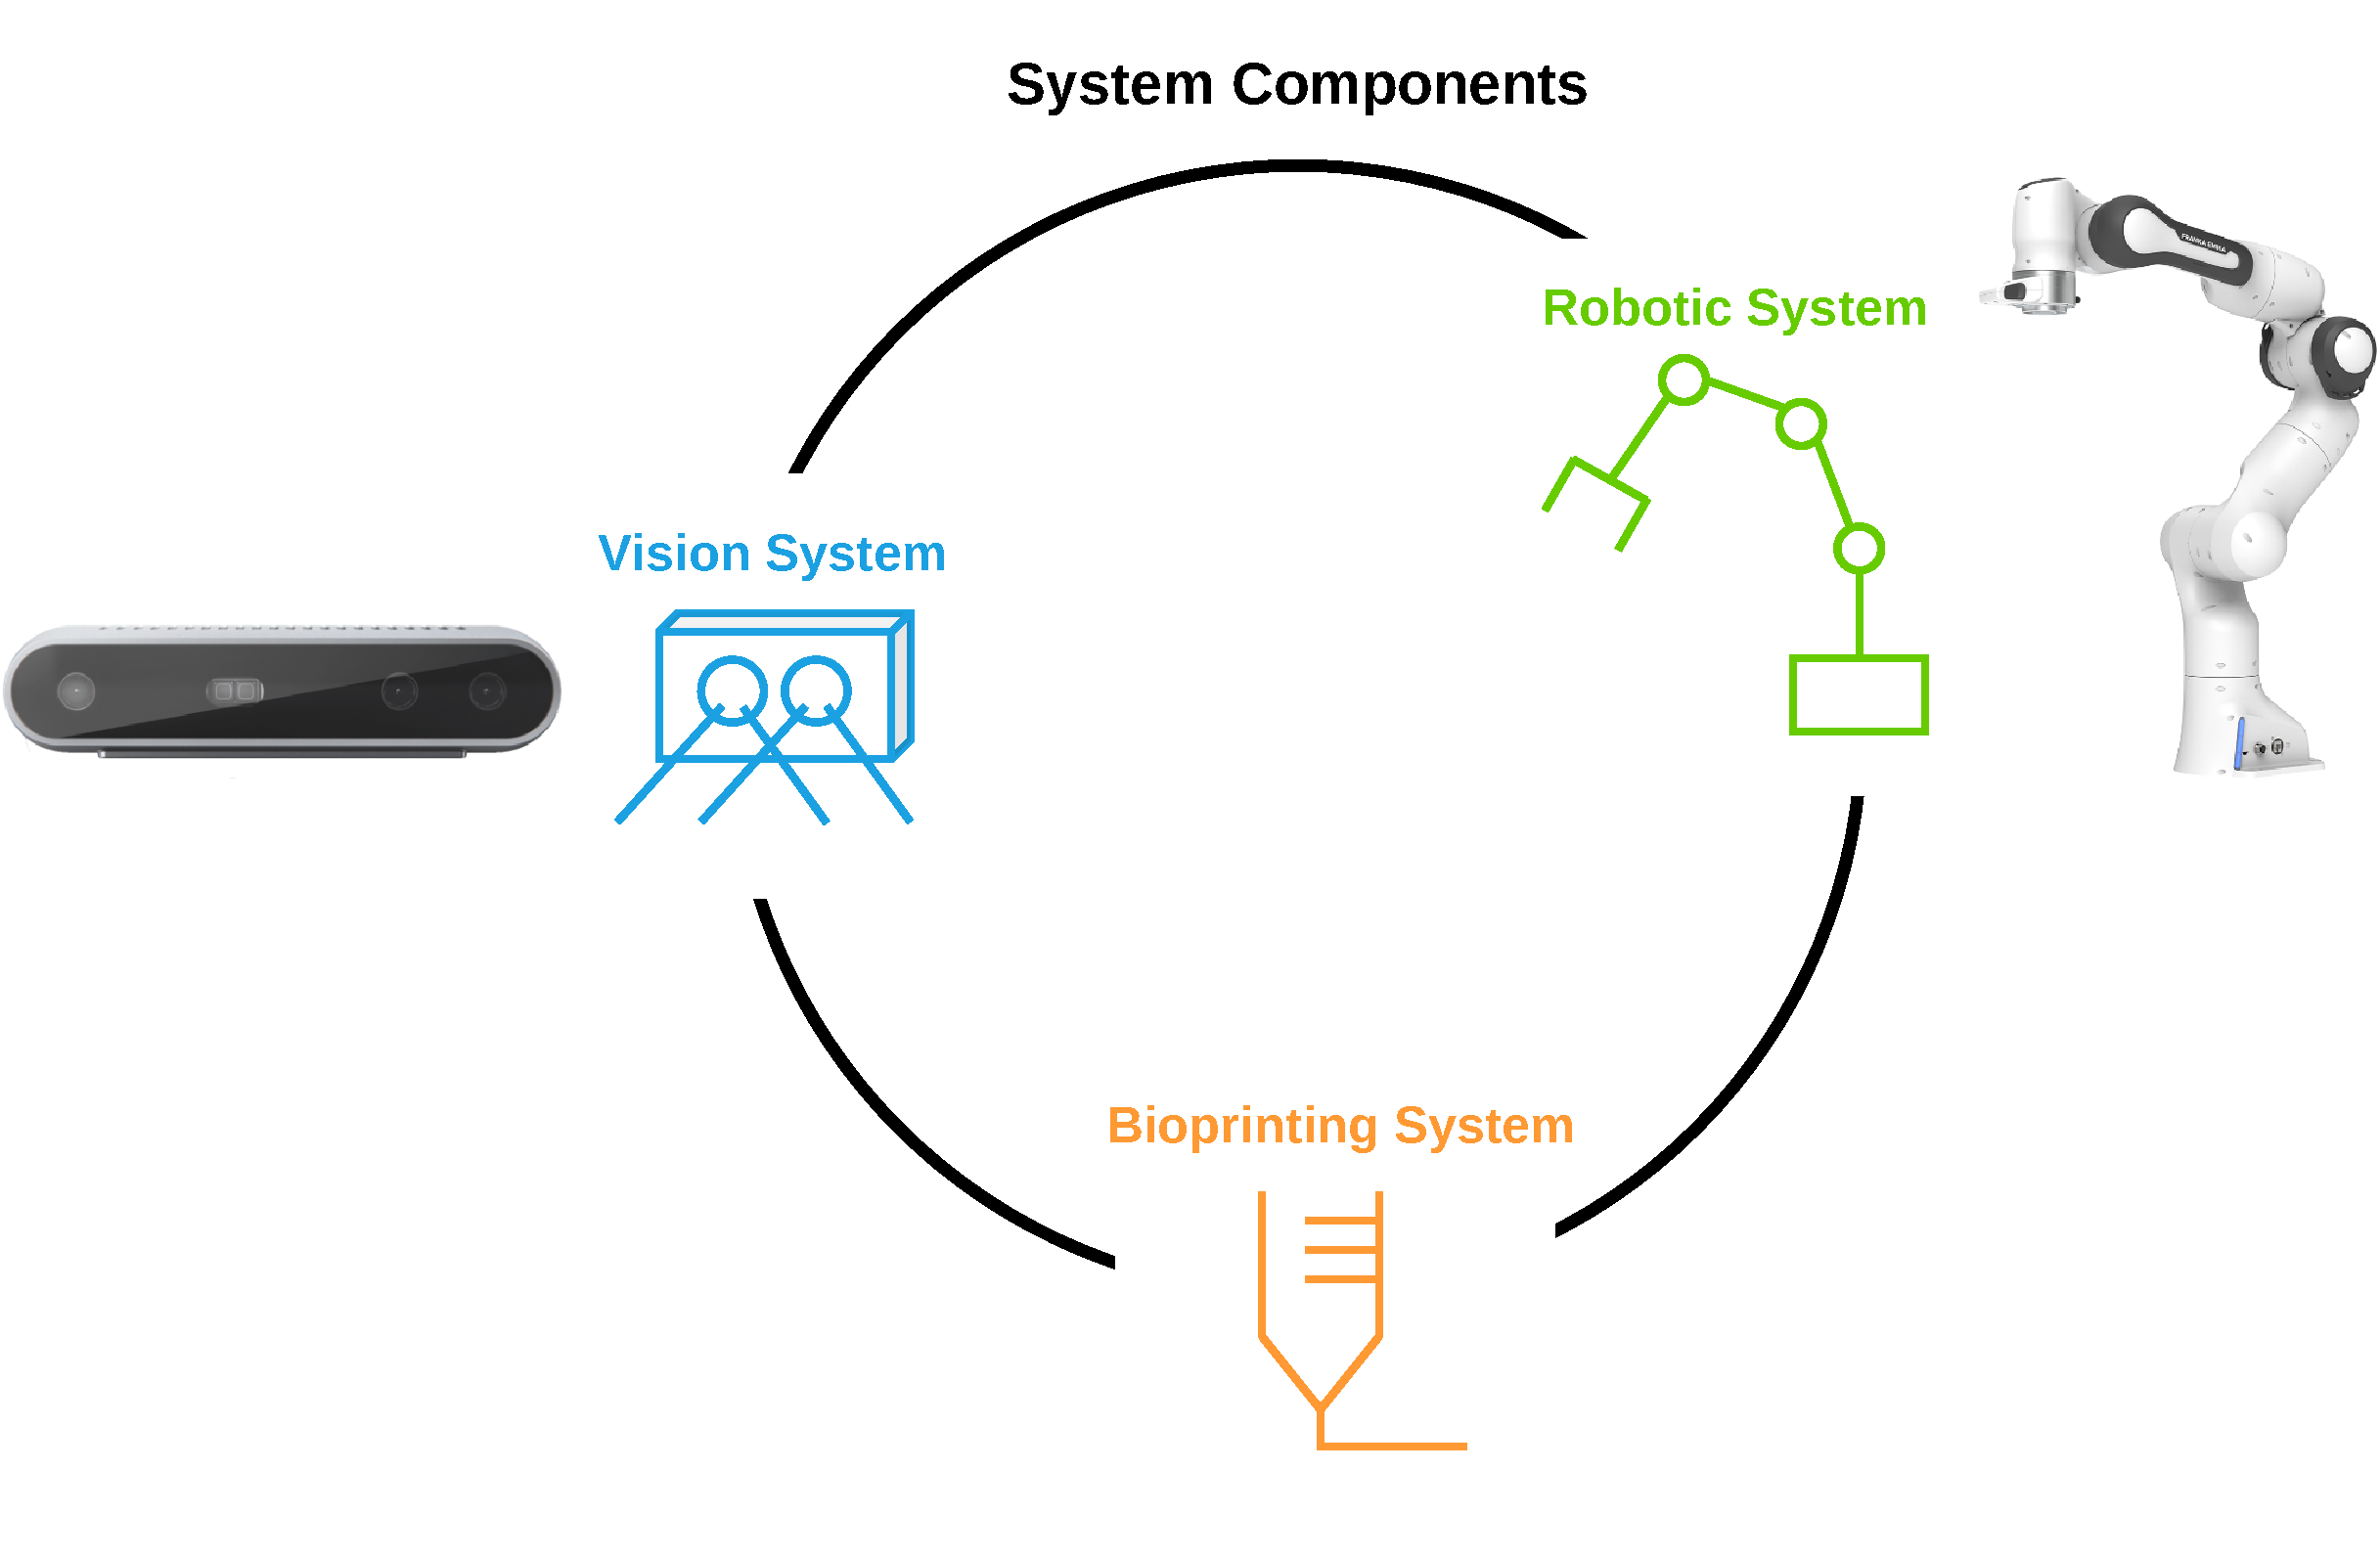
\includegraphics[width=.6\textwidth]{system_architecture_components_complete}
	\caption{System architecture main components. The robotic system is a Panda 7 \gls{dof} robotic manipulator. The vision system is an Intel\textregistered RealSense\texttrademark{} D415 depth camera. The bioprinting system consists of a custom made syringe pump print head.}
	\label{fig:system_architecture_components}
\end{figure}

\subsection*{Robotic System}
\label{subsec:system_architecture_components_robotic_system}

The robotic system is a Panda 7 \gls{dof} robotic manipulator, from Franka Emika. By having seven degrees of freedom this robot is inherently redundant for any task in 3D space.

This is the case because to fully describe an object in space at least six degrees of freedom are need. Three degrees define the position, i.e., the x, y and z coordinates in relation to a reference frame. The other three degrees define the orientation. For example, the three Euler angles ($\alpha, \beta, \gamma$) suffice for orientation definition. It means that position redundancy and orientation requirements are naturally satisfied.

In terms of resolution, this robotic manipulator guarantees 100 \si{\micro\meter}. It matches the normal resolution of extrusion-based bioprinting methods.\\

The robot is relatively light in comparison with industrial robots. It weights almost 18 kg in total but only 13 kg are movable mass. The body is metallic. The safety during operation must be considered at all times. With cartesian speeds up to 2 \si{\meter\per\second}, a collision with the patient/operator can cause severe injuries. In alignment with the requirements, this robot gives control on the speed and acceleration limits.

Regarding its size, it has a maximum reach of 855 mm, which provide a good reach to interact with a patient lying down on a bed, if the robot is at bedside. It is not a small arm but it is not very bulky. It can fit an hospital room but it will demand a certain space, about a meter radius, for safety reasons.

This robot is powered by normal mains power, 100-240 VAC, which eases the installation process. It also features a safety shutdown mechanism that removes power from the whole system. \\

The robot characteristics described are documented on the robot datasheet, annex \ref{ann:panda_datasheet}. The whole robotic system is thoroughly described on chapter \ref{cha:robotic_system}.

% subsection system_architecture_components_robotic_system

\subsection*{Vision System}
\label{subsec:system_architecture_components_vision_system}

An Intel\textregistered RealSense\texttrademark{} D415 depth camera was used as the vision system. Being a depth camera, it provides not only \gls{rgb} data but also depth data.\\

With \gls{rgb} data, the system is able to apply computer vision algorithms to that data in order to detect a wound within the camera \gls{fov}. If only a \gls{rgb} camera was used, it would only be possible to get information about the wound position in 2D space. That is why the depth functionality comes into play.

The depth sensors will allow the detection of the distance of each pixel in relation to the camera reference frame. With that, a full 3D position in space can be obtained. This means the wound classification requirements are satisfied. The other positive aspect of having depth data is that point clouds can be generated out of it. With a point cloud, it is possible to create meshes of the surfaces detected and do some form of geometric analysis.\\

The vision system is thoroughly described on chapter \ref{cha:vision_system}.

% subsection system_architecture_components_vision_system

\subsection*{Bioprinting System}
\label{subsec:system_architecture_components_bioprinting_system}

The bioprinting system consists of a custom made robot end-effector which works as an extrusion-based print head. The concept is based on a syringe pump mechanism. Several projects served as inspiration for the design of the system \cite{Wijnen2014_open_source_syring_pump_library,Pusch2018_large_volume_syringe_pump_extruder_desktop_3d_printers,Booeshaghi2019_principles_open_source_bioinstrumentation_poseidon}.\\

The \gls{ebb} method was chosen, because it offers the best scalability at this point in time \cite{Vijayavenkataraman2018_bioprinting_tissues_organs_regen_med}. Although the resolution is the worst among the three methods, our particular application does not really need better resolution. Besides, its resolution is closer to that of the robotic system. Finally, it is the easiest and cheapest method to build.

Regarding some of the requirements, the extrusion-based systems allows us to use big volume containers; have a wide diversity of compatible bioinks for various tissues  \cite{Hospodiuk2017_bioink_comprehensive_review_bioprintable_materials}; and still guarantees a fairly good printing speed (see table \ref{tab:system_architecture_requirements_bioprinting_methods_comparison}).\\

This system was developed more to provide comparable data of the bioprinting process, than really to present an innovative extrusion-based print head. The bioprinting system is thoroughly described on chapter \ref{cha:bioprinting_system}.

% subsection system_architecture_components_bioprinting_system

% section system_architecture_components

% ==========================
% = Functional Diagrams =
% ==========================

\section{Functional Diagrams}
\label{sec:system_architecture_functional_diagrams}

At this point it is important to understand how the system components interact with each other. A set of functional diagrams show this interaction, i.e., how the components communicate to exchange data and commands to attain the final goal of a working system.

Figure \ref{fig:system_architecture_functional_diagram_overview} presents an overview of the main components interactions. Each of the main components, robotic, vision, and bioprinting systems communicate to a central control system. This central control system is a computer that runs the software application which communicates with the other systems.

\begin{figure}[htbp]
	\centering
	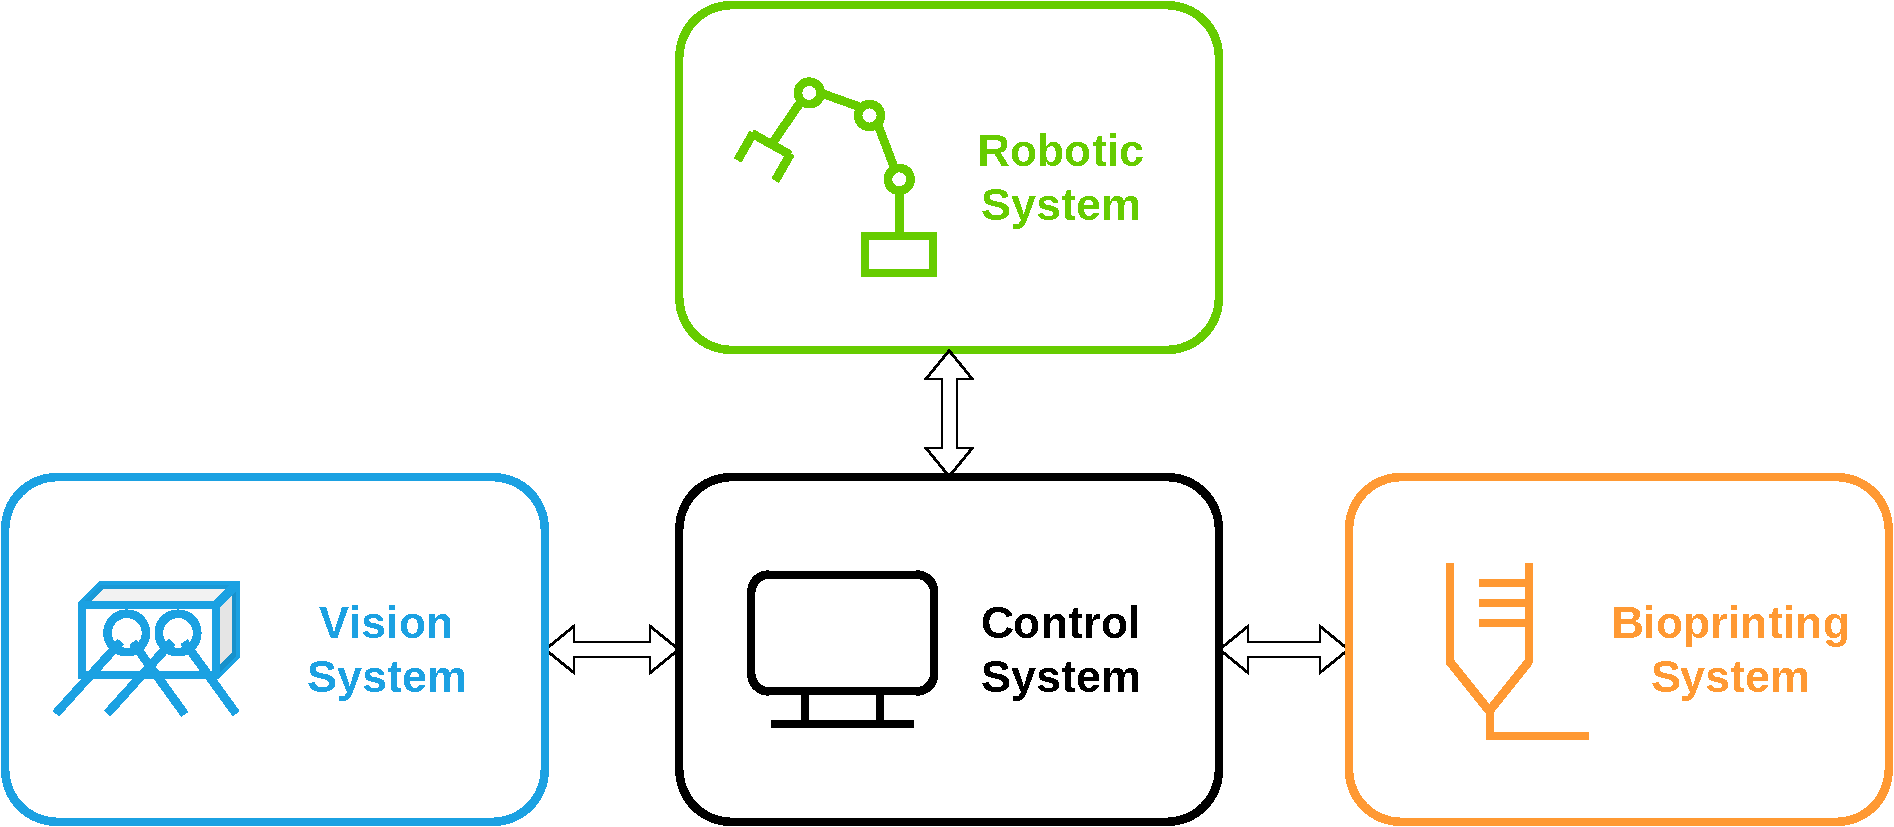
\includegraphics[width=\textwidth]{system_architecture_functional_diagram_overview}
	\caption{System architecture functional diagram overview. It shows the communication interaction between the different components.}
	\label{fig:system_architecture_functional_diagram_overview}
\end{figure}

The robotic, vision, and bioprinting systems, are basically hardware and firmware/software that control the systems themselves and define the communication protocols and data exchange.\\

The robotic system has two main pieces of hardware. The robotic arm and a control unit. They communicate with each other by a proprietary protocol. The robotic arm is mainly hardware and firmware. The control unit is a computer itself running an operating system and control software (Fig. \ref{fig:system_architecture_functional_diagram_robotic_system}).

The control system communicates with the robotic system via the robotic system's control unit through the Ethernet protocol, exchanging control commands and kinematics/dynamics data (Fig. \ref{fig:system_architecture_functional_diagram_robotic_system}).

The robotic system internal architecture is the manufacturer's responsibility. More detailed information on this system is provided on chapter \ref{cha:robotic_system}.

\begin{figure}[htbp]
	\centering
	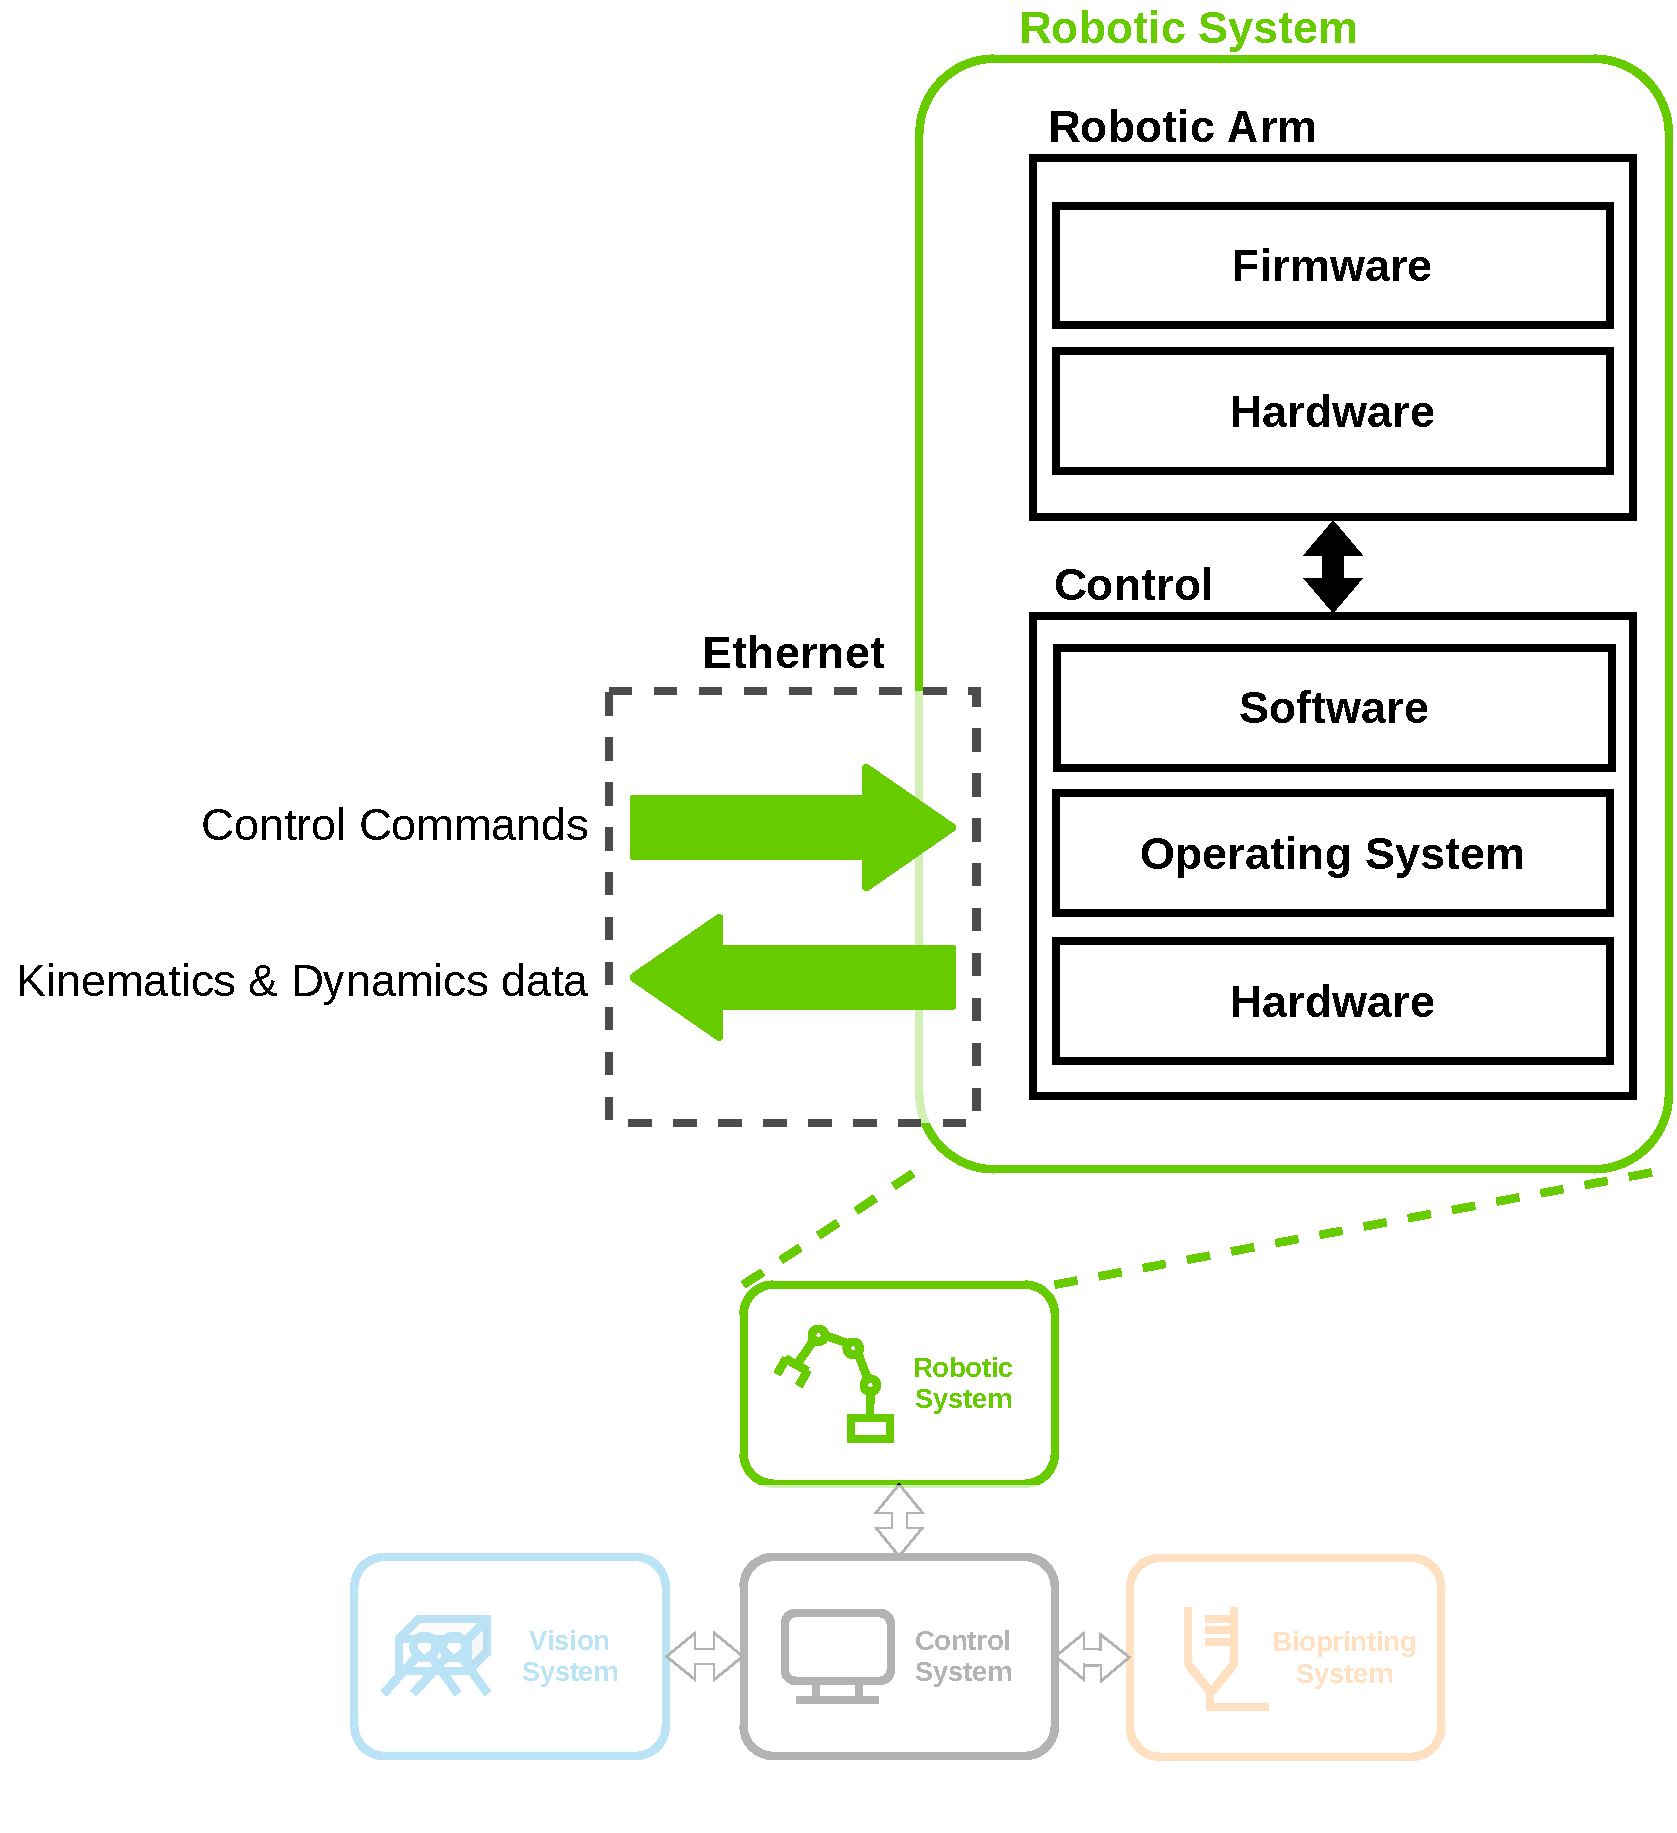
\includegraphics[width=0.6\textwidth]{system_architecture_functional_diagram_robotic_system}
	\caption{System architecture functional diagram of the robotic system. The robotic system is made of two hardware parts that communicate with each other. The global control system communicates with the robotic system via the robotic system's control unit using the Ethernet protocol.}
	\label{fig:system_architecture_functional_diagram_robotic_system}
\end{figure}

The vision and bioprinting systems have a similar internal architecture. The vision system consists on the depth camera composed by an hardware layer and a firmware layer (Fig. \ref{fig:system_architecture_functional_diagram_vision_bioprinting_system} left). The latter controls the hardware and implements the communication protocol via \gls{usb}. The whole architecture was developed by the manufacturer.

For a more detailed description of the vision system, refer to chapter \ref{cha:vision_system}.\\

The bioprinting system, as previously mentioned, consists on a custom made print head. Its architecture, the hardware and firmware layers were developed on this thesis. The communication interface used was also \gls{usb}. The communication \gls{api} allows the control system to inquiry about the available bioink volume and send commands to control the bioink dispensing (Fig. \ref{fig:system_architecture_functional_diagram_vision_bioprinting_system} right).

For the complete description of the bioprinting system, refer to chapter \ref{cha:bioprinting_system}.

\begin{figure}[htbp]
	\centering
	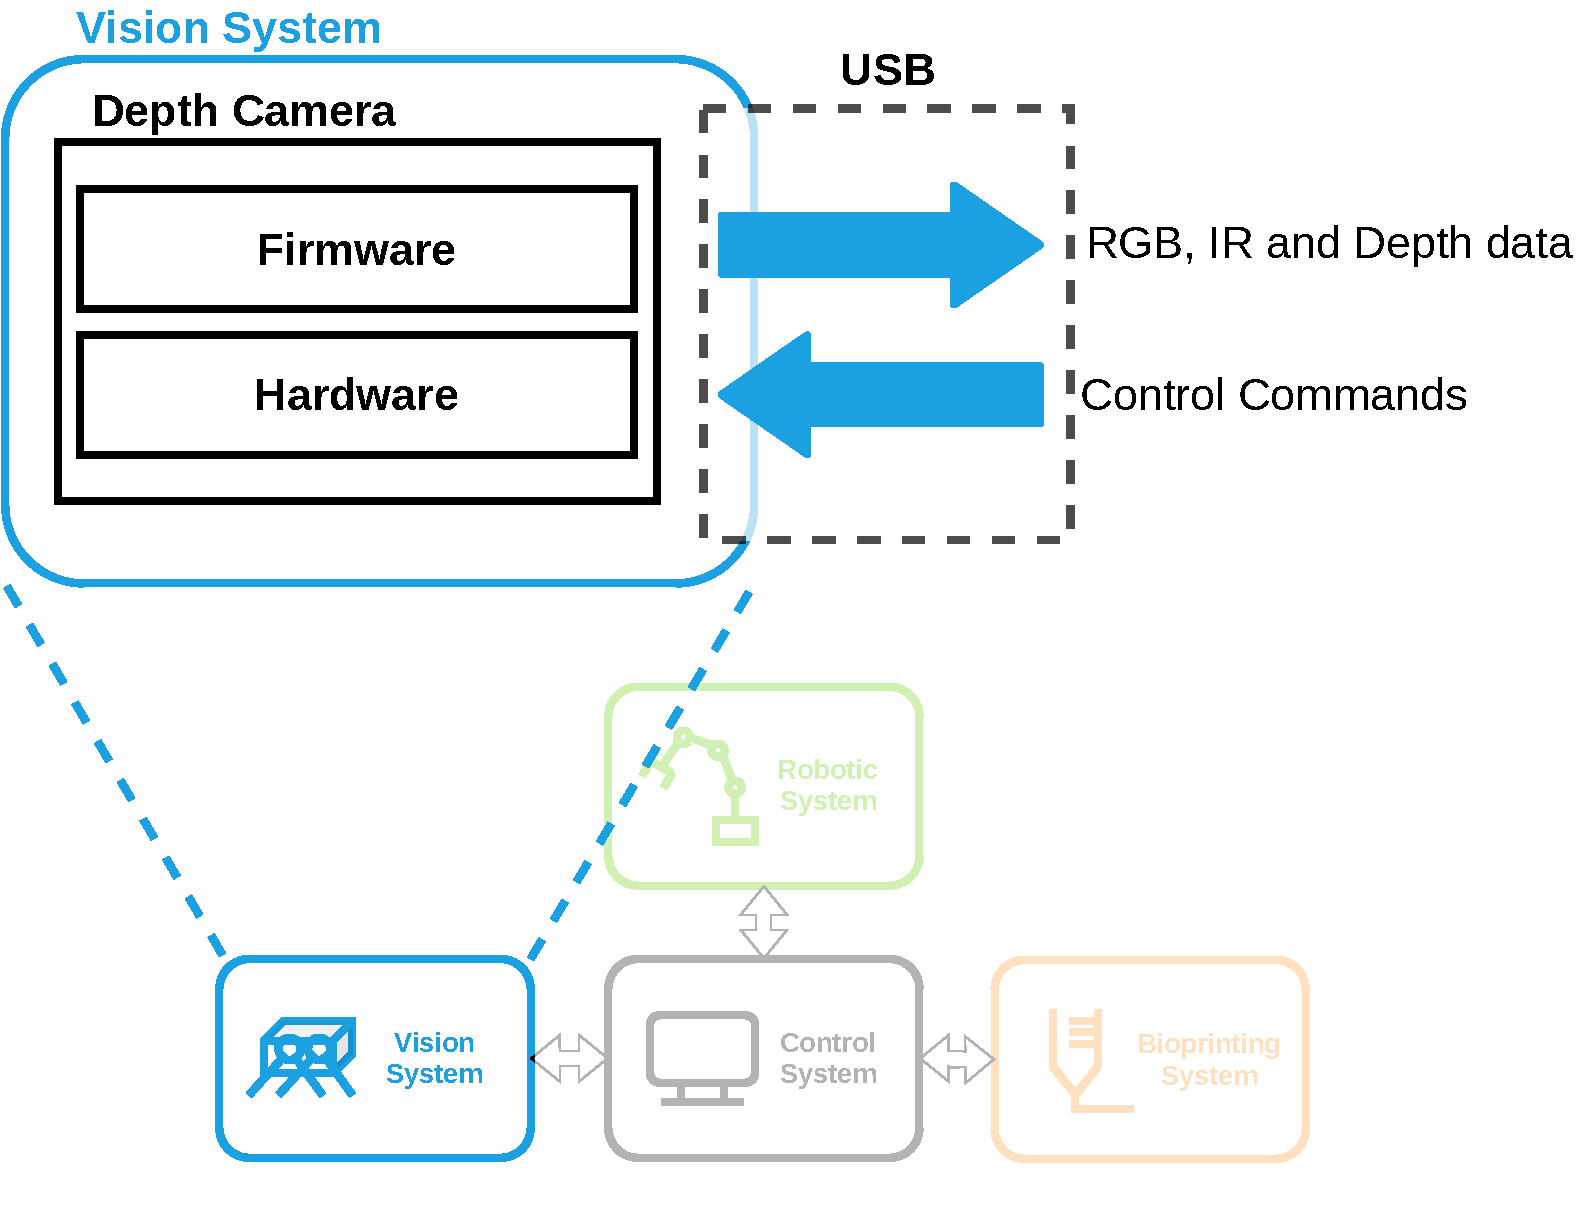
\includegraphics[width=0.45\textwidth]{system_architecture_functional_diagram_vision_system}
	\hspace{0.1in}
	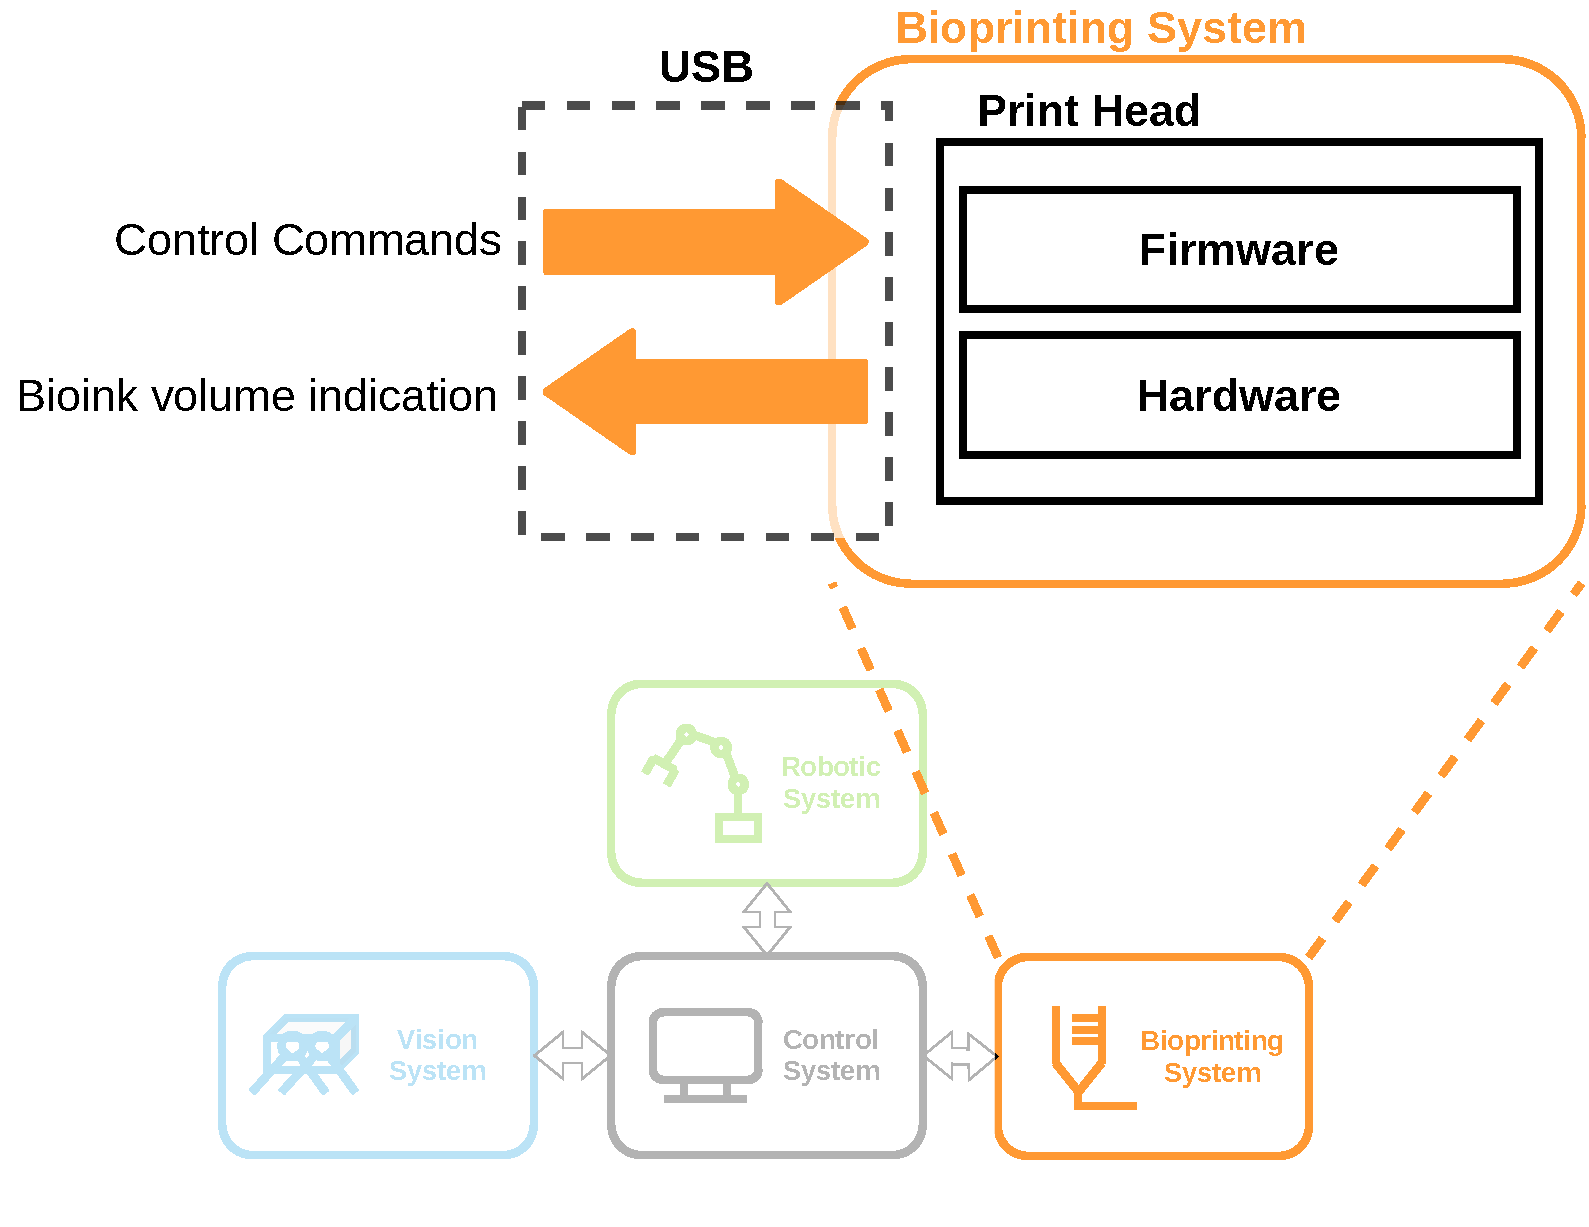
\includegraphics[width=0.45\textwidth]{system_architecture_functional_diagram_bioprinting_system}
	\caption{System architecture functional diagrams of the vision (left) and bioprinting (right) systems. Both systems share a similar architecture. They have only hardware and firmware layers. The vision system architecture is manufacturer dependent, and the bioprinting was custom made within this thesis work.}
	\label{fig:system_architecture_functional_diagram_vision_bioprinting_system}
\end{figure}

Finally, the control system's architecture consists on several layers like: (a) the common layers of a personal computer, the hardware and operating system layers; (b) a middle-ware layer, \gls{ros}; and (c) an application layer, which consists on the main work of this thesis (Fig. \ref{fig:system_architecture_functional_diagram_control_system}).

The application layer was built directly on top of \gls{ros} which means it is completely dependent on its existence. The reason this is done this way is because both the robot and the camera have \gls{ros} integrations. Besides, \gls{ros} uses a distributed architecture that eases the communication between the different nodes. An overview description of \gls{ros} is provided on Annex \ref{ann:ros}.

The application itself is composed of several layers, each belonging to a specific system (Fig. \ref{fig:system_architecture_functional_diagram_control_system}). In operational terms, they all stack up, like shown on Figure \ref{fig:system_architecture_intro} (right), passing data to the top adjacent layer. Some layers belong to the same \gls{ros} package and can even belong to the same node. In general, a system is represented by a package but not necessarily.

\begin{figure}[htbp]
	\centering
	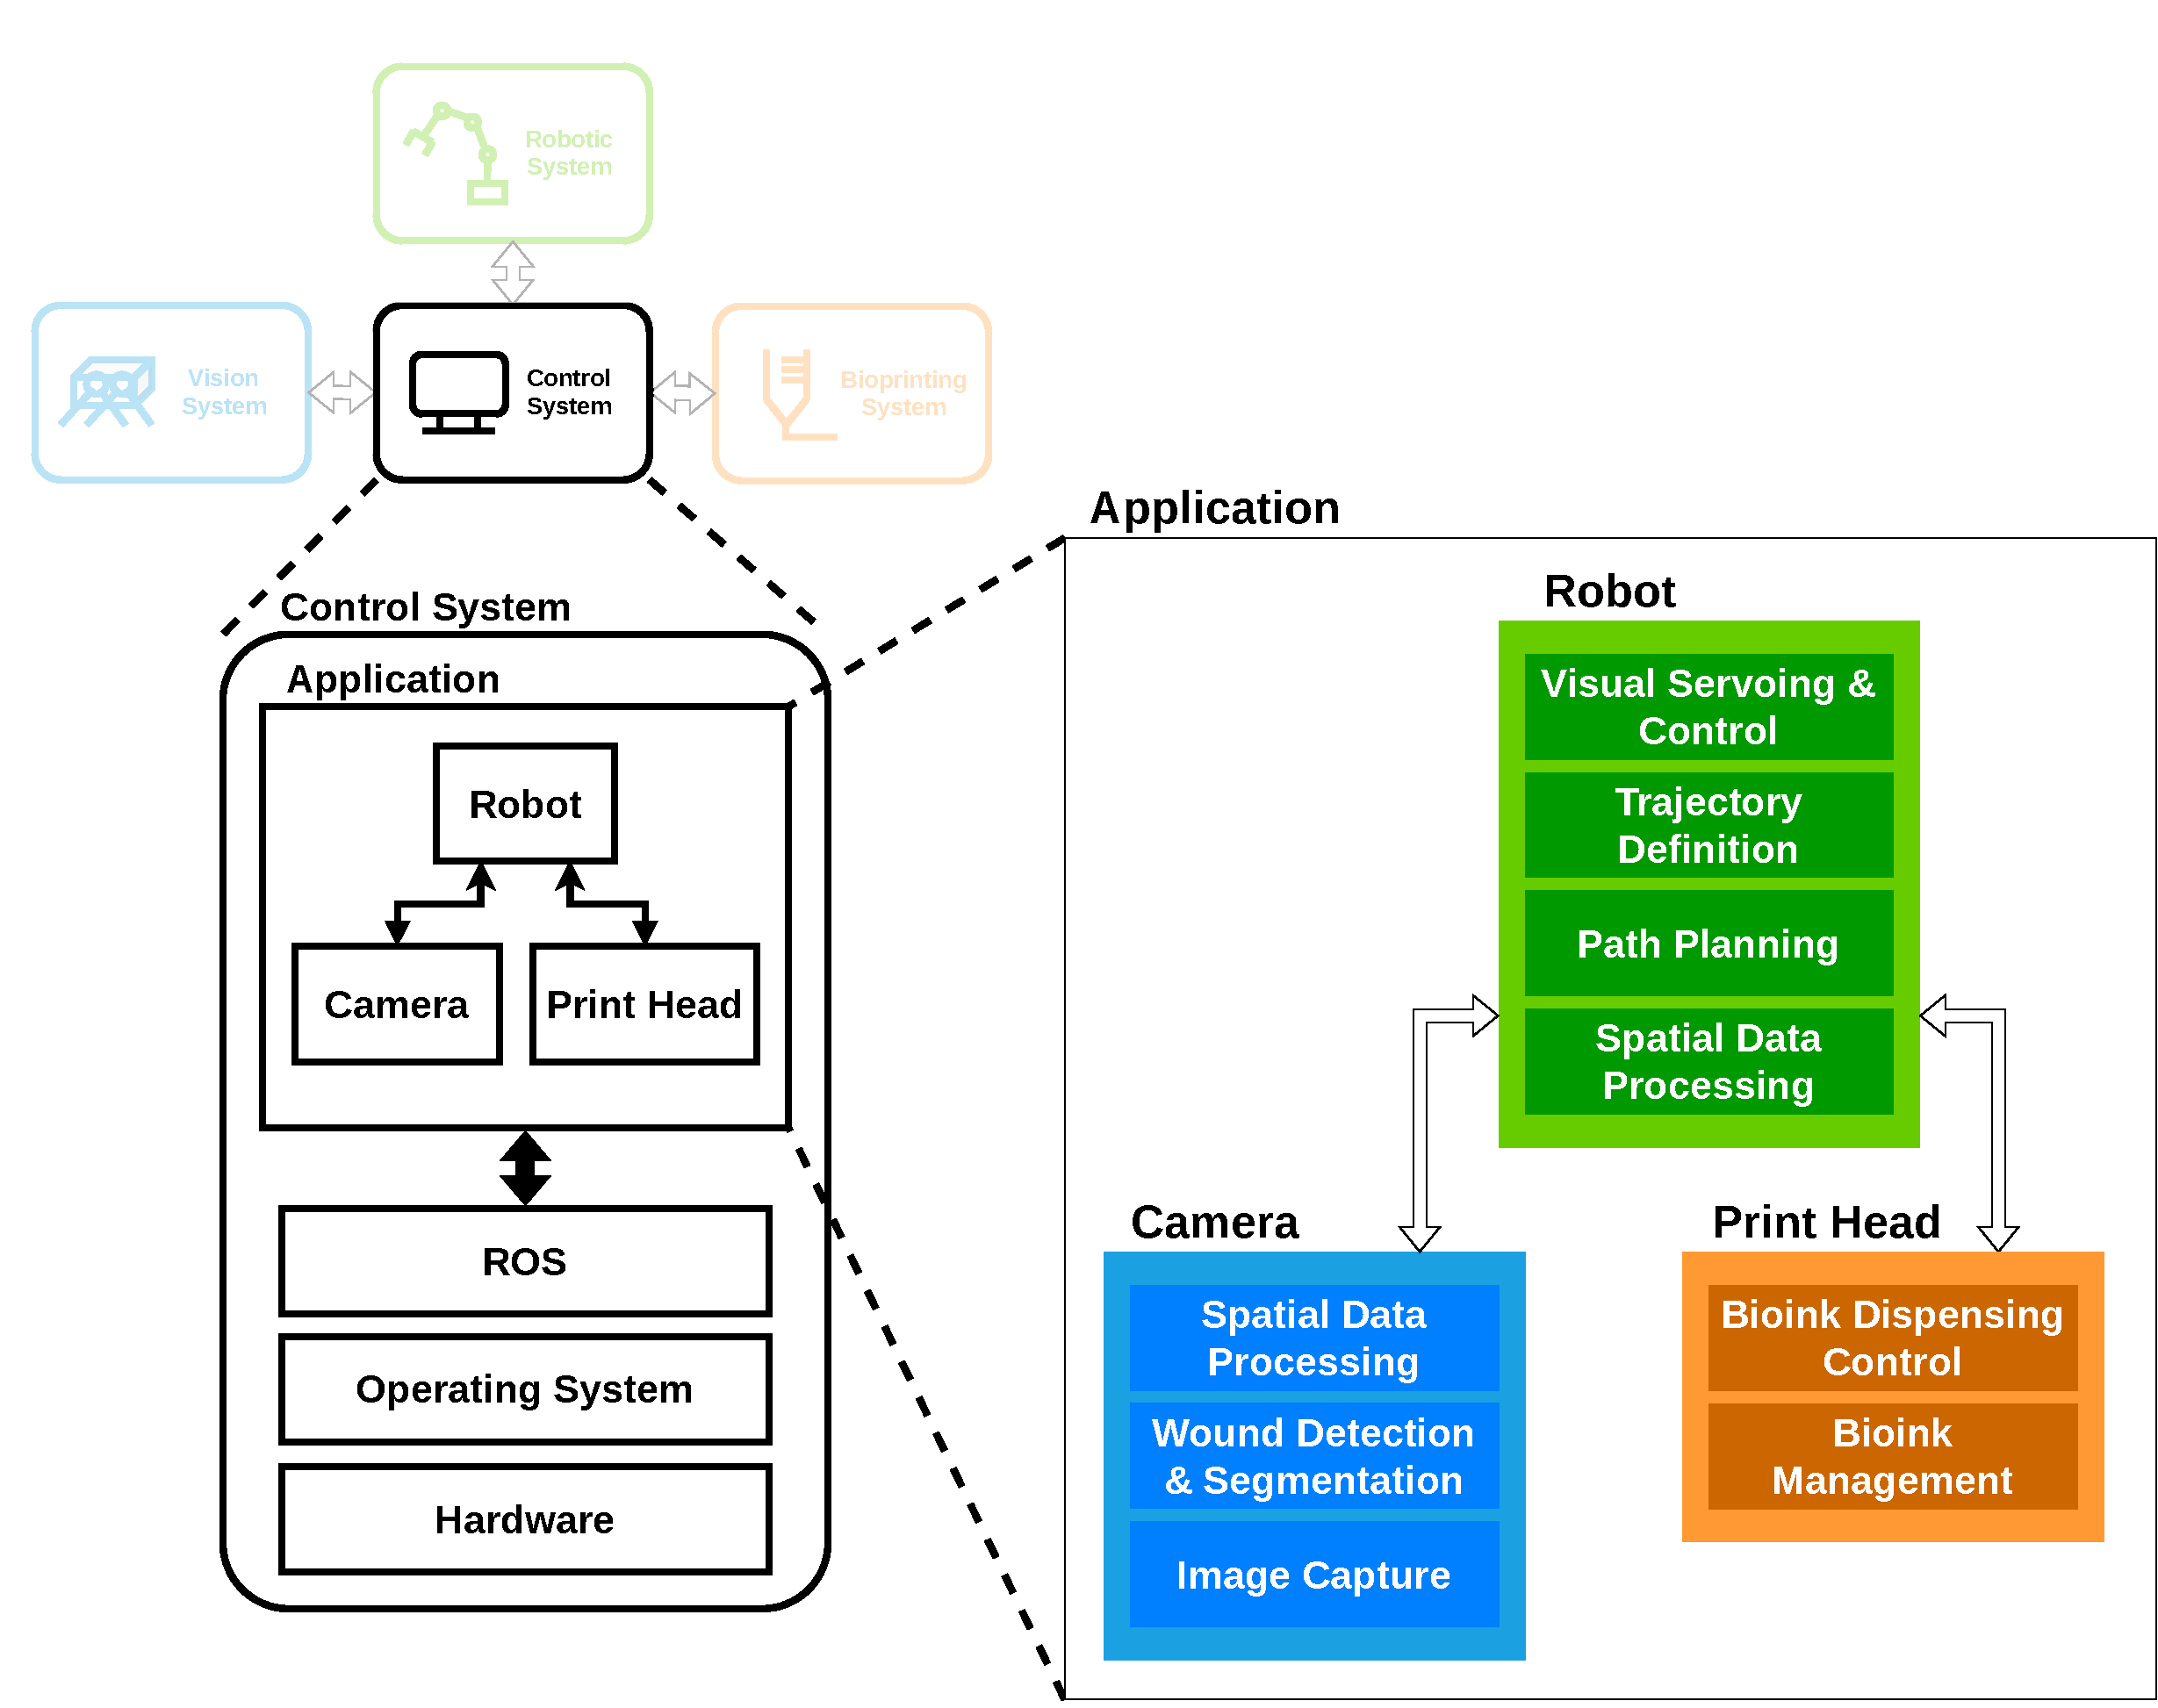
\includegraphics[width=0.9\textwidth]{system_architecture_functional_diagram_control_system}
	\caption{System architecture functional diagram of the control system. It is composed by the normal computer layers, hardware and operating system, plus a middle-ware layer, \gls{ros}. On top of \gls{ros} runs the main application that controls the whole system. This application is composed by several layers related to the other system components.}
	\label{fig:system_architecture_functional_diagram_control_system}
\end{figure}

Each layer is documented in detail on section \ref{sec:system_architectural_layers}.

% section system_architecture_functional_diagrams

% ==========================
% = Architectural Layers =
% ==========================

\section{Architectural Layers}
\label{sec:system_architectural_layers}

Nine layers compose the control system application. Next, they will be thoroughly described. Figure \ref{fig:system_architecture_layers_detail} presents a more detailed view of the layers composition and inter-layer communication.

\begin{figure}[htbp]
	\centering
	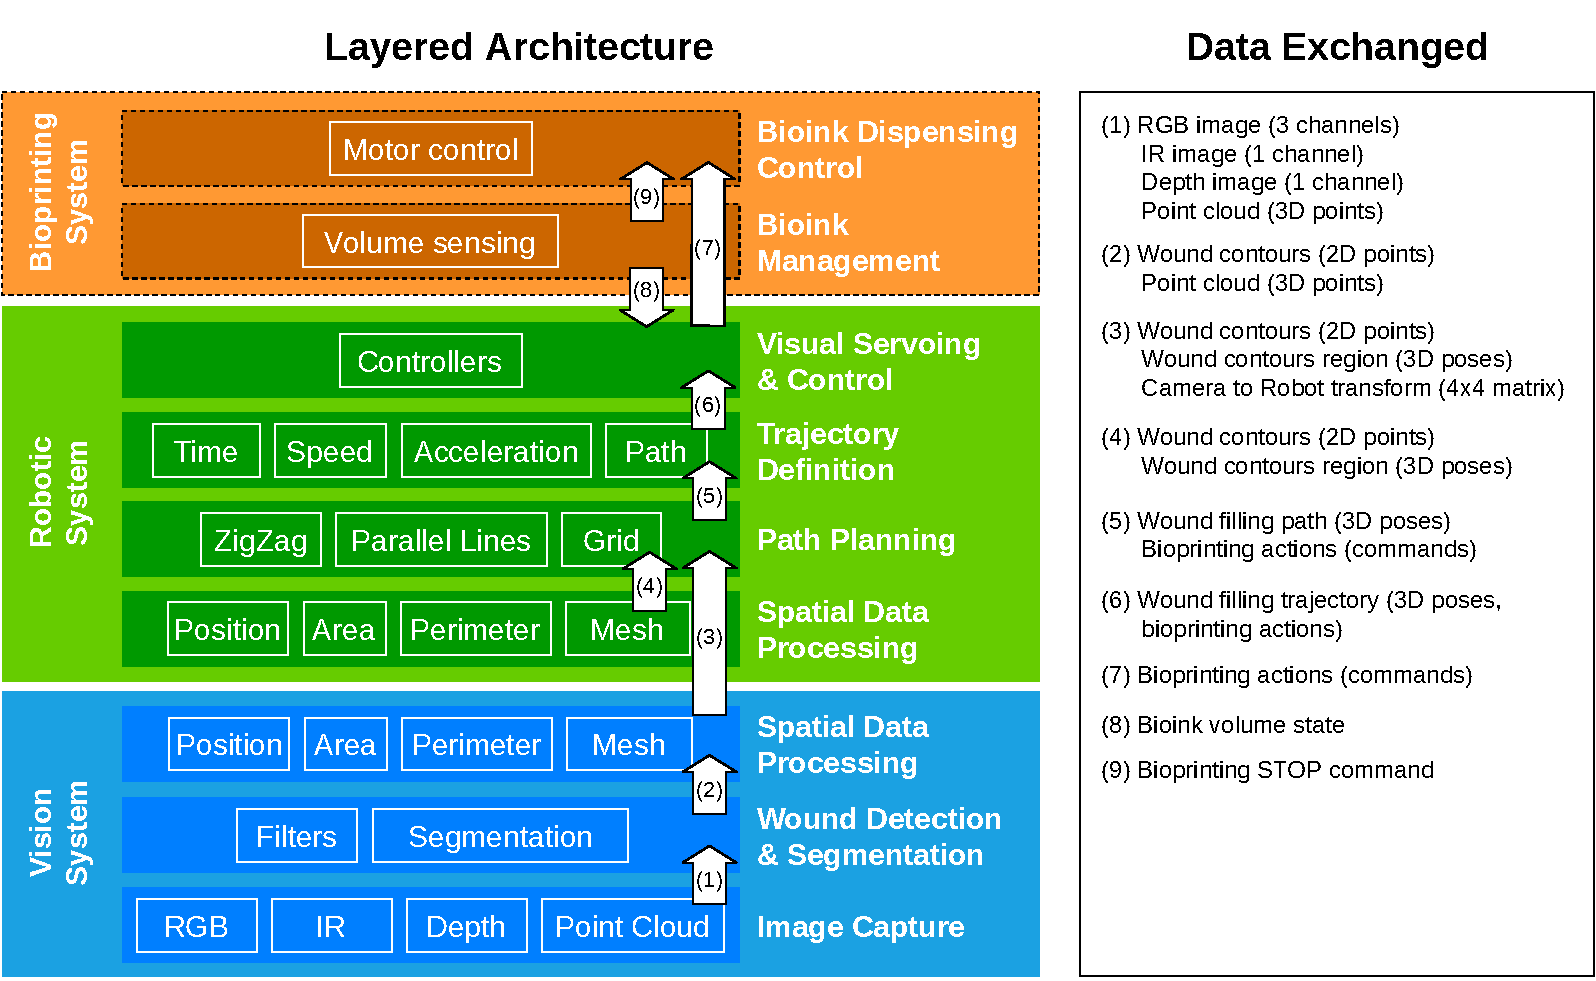
\includegraphics[width=\textwidth]{system_architecture_layers_detail}
	\caption{System's architectural layers detail. Each layer shows their internal blocks which corresponds to the data gathered or the type of actions taken on that layer. The arrows represent the inter-layer interaction. On the \textit{Data Exchanged} area the data types that are exchanged between layers are listed. }
	\label{fig:system_architecture_layers_detail}
\end{figure}

\subsection{Camera Layers}
\label{subsec:system_architectural_camera_layers}

The camera layers are responsible for obtaining wound data out of the camera image stream. That data will then be used by the robotic arm to guide the print head through the wound filling bioprinting procedure.

\subsubsection*{Image Capture}
\label{subsubsec:system_architectural_camera_layers_image_capture}

This layer is responsible for tapping into the camera image stream. Figure \ref{fig:system_architecture_layer_image_capture_flowchart} presents the flowchart of this layer.\\

\begin{figure}[htbp]
	\centering
	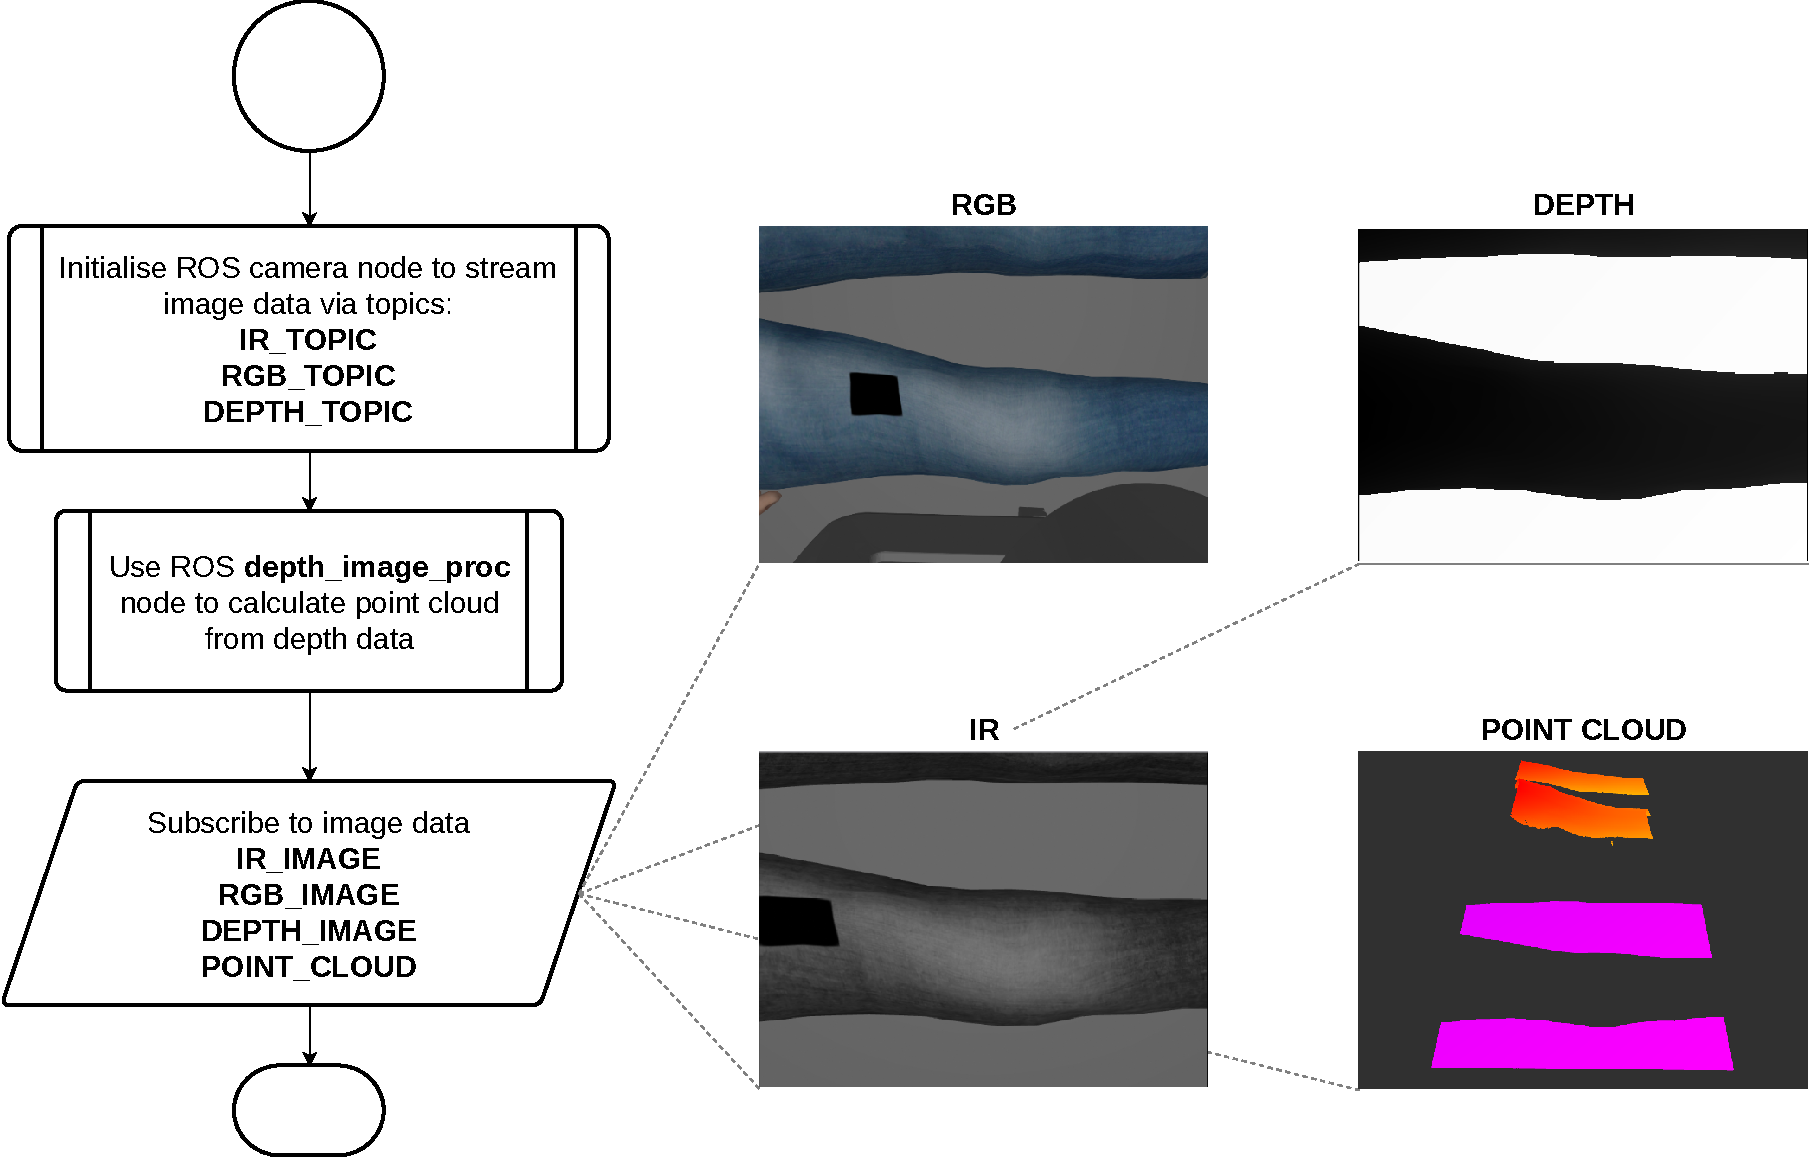
\includegraphics[width=\textwidth]{system_architecture_layer_image_capture_flowchart}
	\caption{Image capture flowchart. The camera connection is established via a \gls{ros} node which handles the image data streaming via \gls{ros} topics. Using the depth data, the depth\_image\_proc nodelet is used to create a point cloud and stream that data. Finally, the topics are subscribed to tap into the data for future use.
	The example images are from the simulation environment.}
	\label{fig:system_architecture_layer_image_capture_flowchart}
\end{figure}

To communicate with the camera, a \gls{ros} node, provided by the camera manufacturer, is used. This node handles the communication between the camera and the control system computer and provides a data access point via \gls{ros} topics.

Since point cloud data is also important for the system, but it is not provided directly by the camera, a generation method must be used. The depth\_image\_proc \gls{ros} package has that capability. It is used to generate point cloud data from the depth data streamed by the camera.\\

With all the data available via \gls{ros} topics the last step is to subscribe to those topics to have access to the data.

% subsubsection system_architectural_camera_layers_image_capture

\subsubsection*{Wound Detection \& Segmentation}
\label{subsubsec:system_architectural_camera_layers_wound_detection_segmentation}

The wound detection \& segmentation layer is probably the most important layer associated with the camera. At this level the camera becomes really useful and fullfils its purpose, which is detecting a burn wound on its \gls{fov}.

As discussed on section \ref{sec:burn_wound_segmentation}, there are many different algorithms with different complexities and outcomes for wound detection. On this work, for the sake of simplicity and developing the whole process chain, a very simplistic approach was followed. The wound is modelled by a simple black painted shape. With this model a very simple binarisation approach can be used. Figure \ref{fig:system_architecture_layer_wound_detection_segmentation_flowchart} presents the flowchart of wound detection and segmentation.\\

\begin{figure}[htbp]
	\centering
	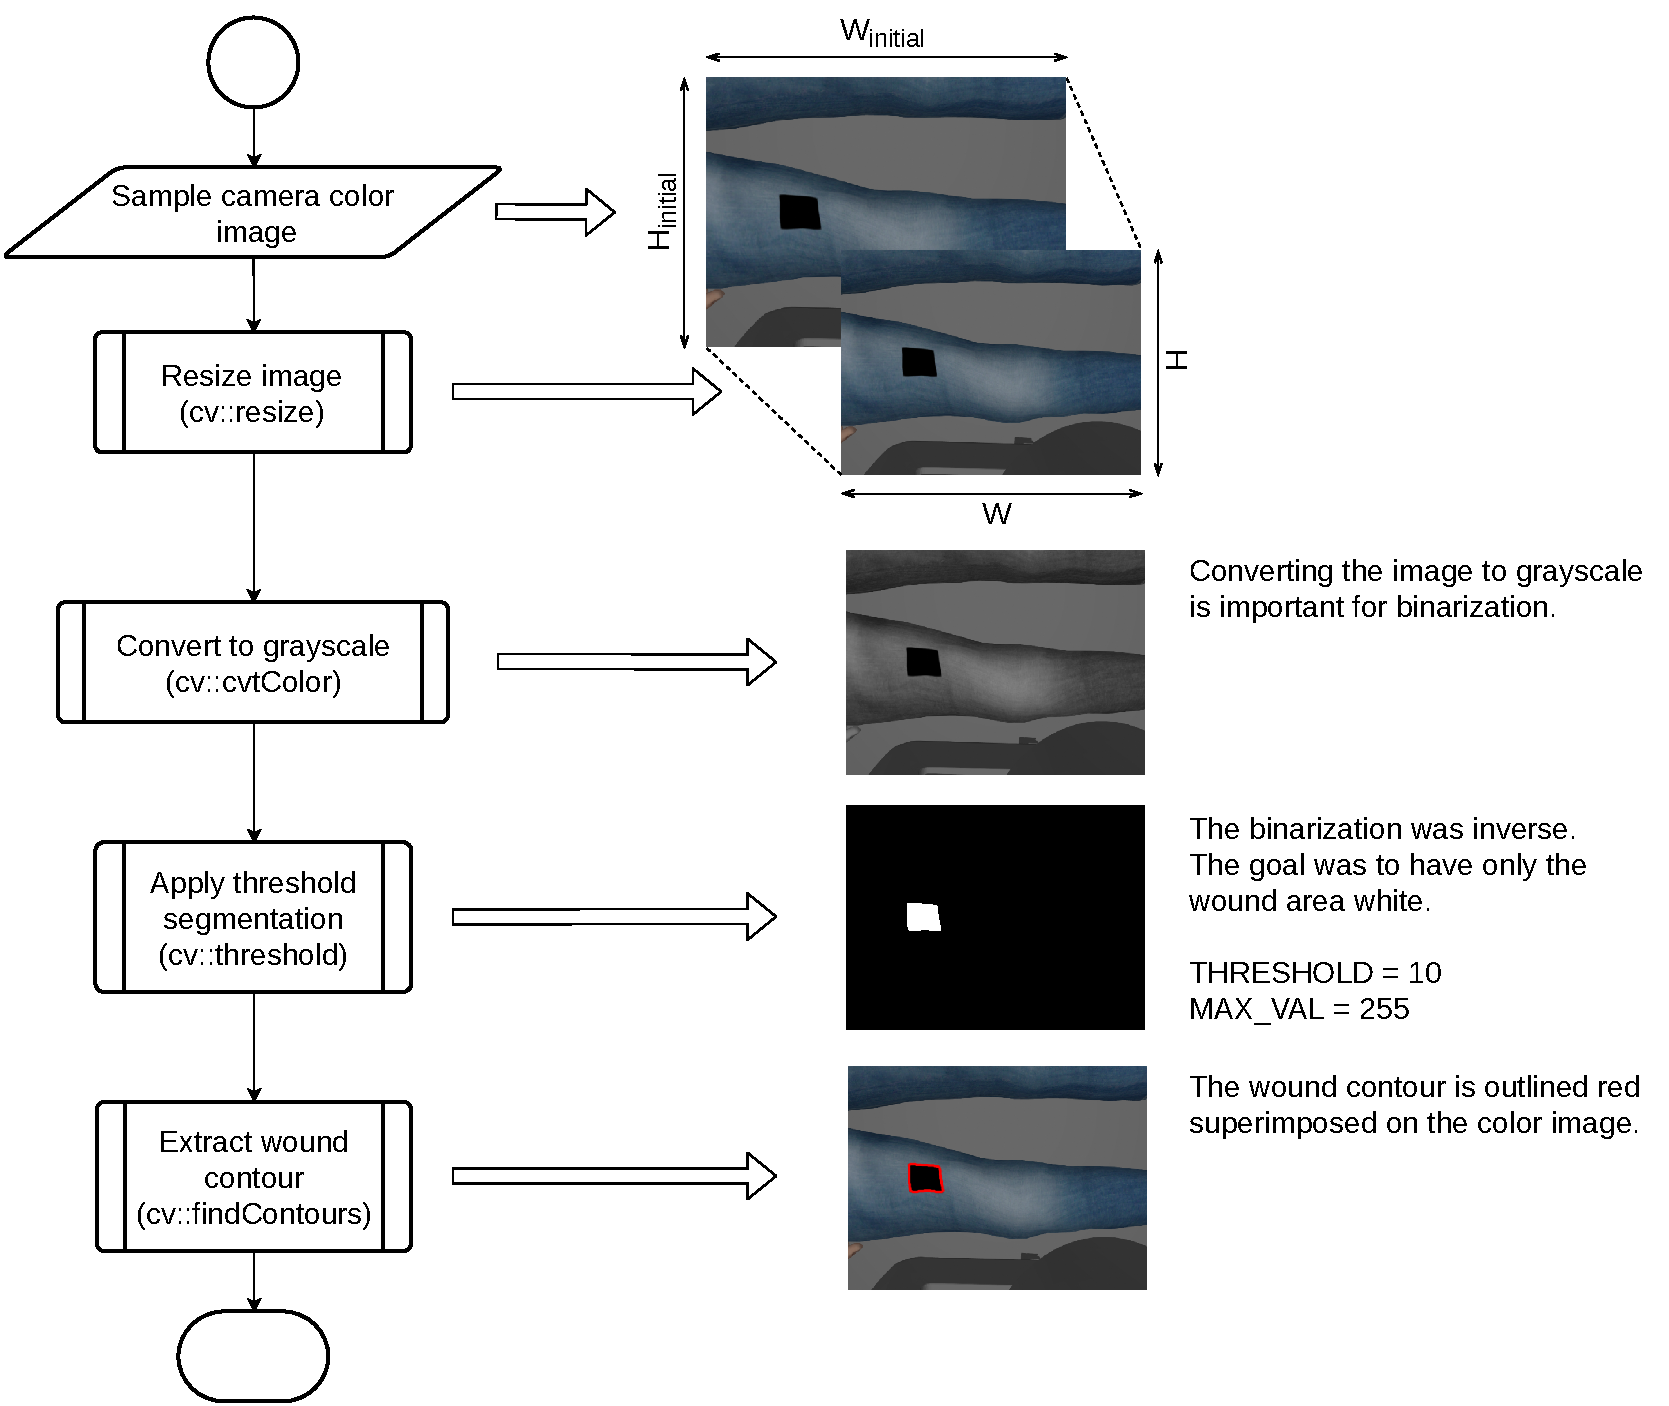
\includegraphics[width=\textwidth]{system_architecture_layer_wound_detection_segmentation_flowchart}
	\caption{Wound detection and segmentation flowchart. It starts by sampling a colour image from the camera and resizing it to a predefined size. Afterwards, the RGB image is converted to grayscale. From there, a binarisation algorithm is applied to segment the wound. Finally, from the binary image the wound contour is obtained.}
	\label{fig:system_architecture_layer_wound_detection_segmentation_flowchart}
\end{figure}

The wound detection is done over the camera RGB data stream. Since we intend to use a binarisation approach, first we need to change the color space from RGB to grayscale. This conversion corresponds to a weighted sum of the three color channels, pixel by pixel (\ref{eq:convertion_rgb_grayscale_general}).

\begin{equation}
\boldsymbol{I}_{GRAY}(x,y) = r * \boldsymbol{R}(x,y) + g * \boldsymbol{G}(x,y) + b * \boldsymbol{B}(x,y)
\label{eq:convertion_rgb_grayscale_general}
\end{equation}

where $r$, $g$ and $b$ are the weights of red, green and blue channels, respectively. The algorithm applied,  OpenCV's \textbf{cvtColor} function, uses the following coefficients \cite{OpenCV2020_color_conversions, ITU2020_grayscale_conversion}: 
$$ r = 0.299, g = 0.587, b = 0.114 $$

After obtaining the grayscale image, a binarisation algorithm is applied to convert the image to black and white. The algorithm uses a threshold value chosen empirically and changes each pixel value according to it. If the pixel value is greater than the threshold it is converted to 0, otherwise to 1. This algorithm used OpenCV's \textbf{threshold} function. For more information on OpenCV functions refer to annex \ref{ann:opencv_functions}.

Because the wound model is a black shape on a lighter background, it is easier to detect the wound contour. The detection is done with OpenCV's \textbf{findContours} function.\\

One of the advantages of this layered structure is that it simplifies the change of implementation of a specific layer leaving the rest of the stack intact. In this particular case, a simplistic algorithm is used to test the whole process chain, but once it is working, another more robust algorithm can be used instead.

% subsubsection system_architectural_camera_layers_wound_detection_segmentation

\subsubsection*{Spatial Data Processing}
\label{subsubsec:system_architectural_camera_layers_spatial_data}

After the wound is detected by the previous layer, this layer is responsible for obtaining spatial data from the wound contour. At this level the wound position, contour area, perimeter and mesh are obtained. Figure \ref{fig:system_architecture_layer_camera_spatial_data_flowchart} presents the flowcharts of spatial data processing.

\begin{figure}[htbp]
	\centering
	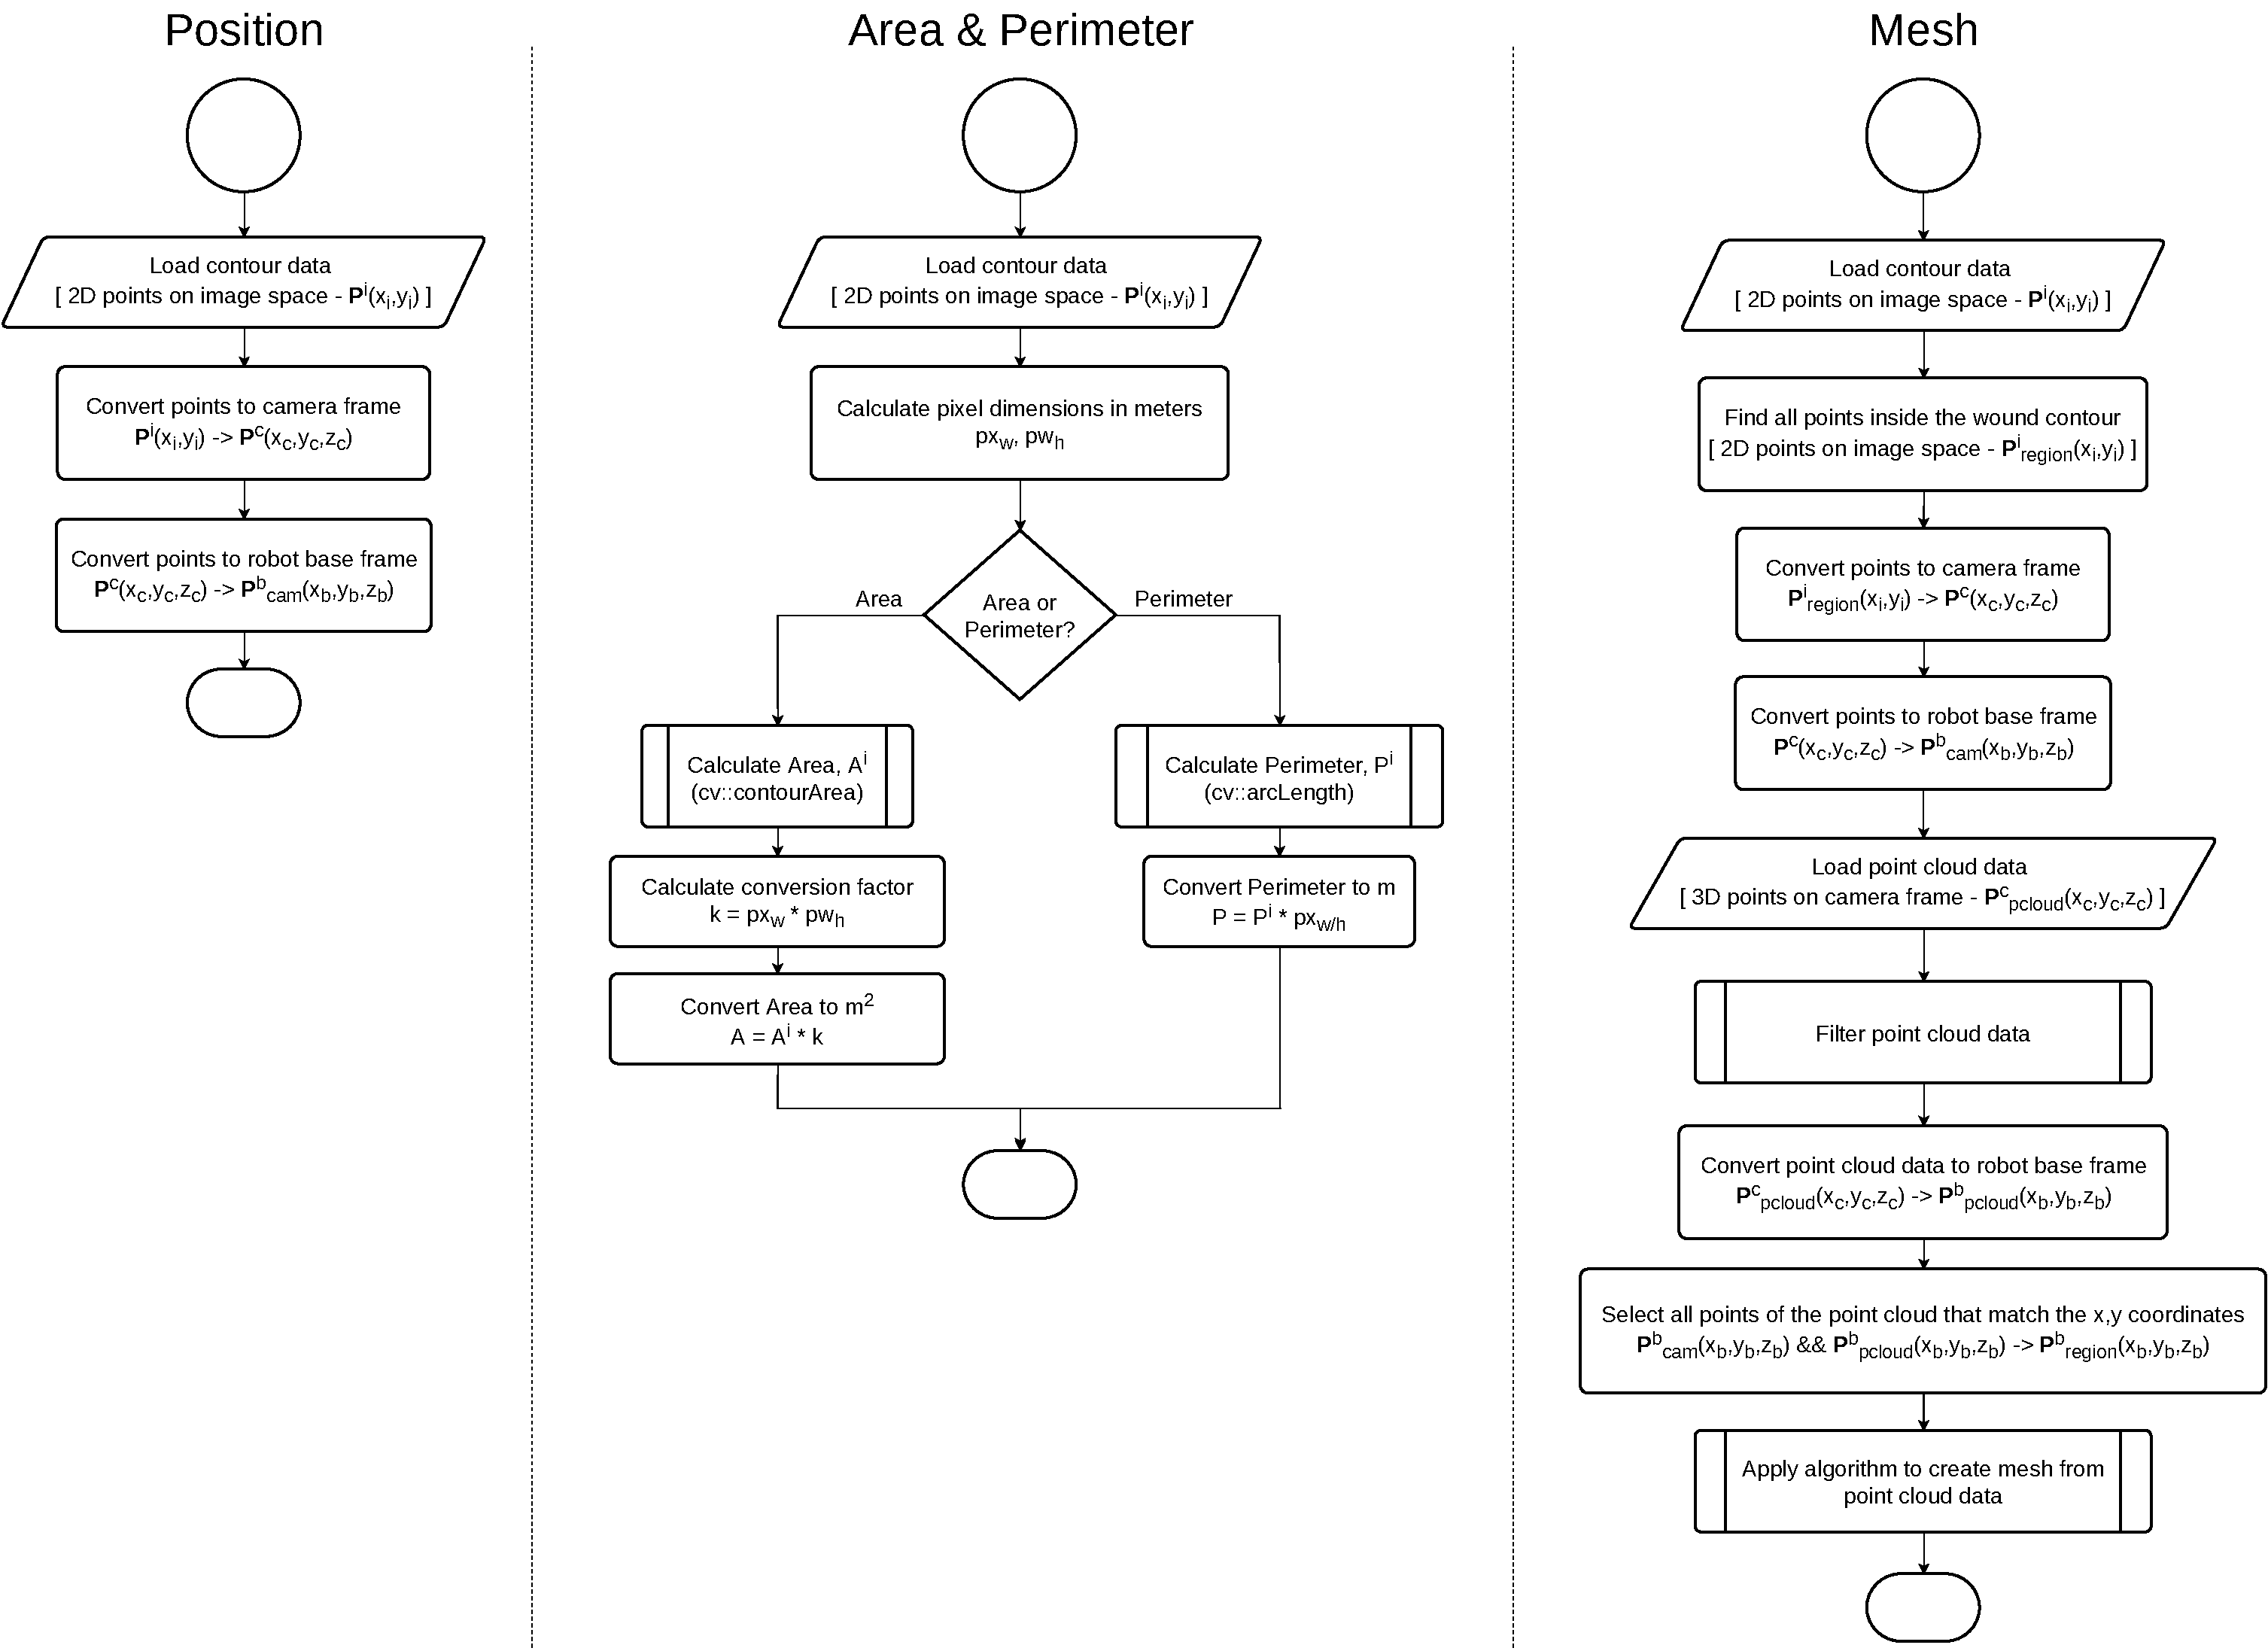
\includegraphics[width=\textwidth]{system_architecture_layer_camera_spatial_data_flowchart}
	\caption{Camera spatial data processing flowcharts. At the left, the flowchart for obtaining wound position. In the middle, the flowchart to calculate the wound area and perimeter. At the right, mesh generation flowchart. Refer to appendix \ref{app:architectural_layers_flowcharts} for full size images.}
	\label{fig:system_architecture_layer_camera_spatial_data_flowchart}
\end{figure}

The position of the wound is given by the contour previously obtained. The contour is a set of 2D points on the image space. To obtain the position of each point in relation to the robot, a transform must be applied between the camera reference frame ($O_cx_cy_cz_c$) and the robot base frame ($O_bx_by_bz_b$).

A point $\boldsymbol{P}^c = (x_c, y_c, z_c)$, on the camera frame, is transformed to point $\boldsymbol{P}^b = (x_b, y_b, z_b)$, on the robot base frame, according to equation \ref{eq:camera_point_transform_robot_base_camera},

\begin{equation}
\boldsymbol{P}^b = \boldsymbol{H}^b_c \boldsymbol{P}^c
\label{eq:camera_point_transform_robot_base_camera}
\end{equation}

where $\boldsymbol{H}^b_c$ is the homogeneous transformation matrix between camera frame and robot base frame. This matrix is obtained via \gls{ros} \textbf{tf} package. Knowing every point of the wound contour allows us to precisely know the wound location.\\

Besides the contour points, points inside the contour area are also obtained for future path planning. The following algorithm, describes in more detail how all the points are converted to the robot base frame:

\begin{enumerate}
    \item Obtain the list of all the contour points and points inside the wound contour, referenced to image space, $\boldsymbol{P}^i(x_i, y_i)$.
    \item Convert these points to camera frame with the z coordinate equal to the distance between the camera and wound, $\boldsymbol{P}^c(x_c, y_c, z_c)$.
    \item Convert the points on camera frame to the robot base frame using equation \ref{eq:camera_point_transform_robot_base_camera}, $\boldsymbol{P}^b_{cam}(x_b, y_b, z_b)$.
    \item Convert the points from point cloud to the robot base frame using equation \ref{eq:camera_point_transform_robot_base_camera}, $\boldsymbol{P}^b_{pcloud}(x_b, y_b, z_b)$.
    \item For each $\boldsymbol{P}^b_{cam}$ point (contour region), search for a $\boldsymbol{P}^b_{pcloud}$ point that is within a small range of the camera point (\ref{eq:point_conversion_valid_range}).
    \item For all the points that match, store the point cloud point as a wound contour region pose, $\boldsymbol{P}^b_{region}(x_b, y_b, z_b)$.
\end{enumerate}

\begin{equation}
\label{eq:point_conversion_valid_range}
    \left.
    \begin{aligned}
    x_{cam} - \delta \le x_{pcloud} \le x_{cam} + \delta\\
    y_{cam} - \delta \le y_{pcloud} \le y_{cam} + \delta
    \end{aligned}
    \right.
\end{equation}\\

The wound area and perimeter are calculated on the image space (px$^2$, px) and converted to robot space (\si{\meter \squared}, \si{\meter}). The conversion factor, $k$, is obtained by relating the image dimensions with the \gls{hfov} at a certain camera distance. $k$ allows to convert the area dimensions. For the perimeter, only $px_w$ or $px_h$ is needed. Equations \ref{eq:px_to_meter_conversion} and \ref{eq:workspace_limits} show the conversion factor calculation.

\begin{equation}
k = px_w \times px_h = (\frac{Y_{max} - Y_{min}}{W}) \times (\frac{X_{max} - X_{min}}{H})
\label{eq:px_to_meter_conversion}
\end{equation}

\begin{equation}
\label{eq:workspace_limits}
    \left.
    \begin{aligned}
        Y_{max} = \frac{W_s}{2} \\
        Y_{min} = \frac{-W_s}{2} \\
        X_{max} = \frac{H_s}{2} \\
        X_{min} = \frac{-H_s}{2} \\
    \end{aligned}
    \right.
\end{equation}

The quantities $W_s$ and $H_s$ represent the width and height, respectively, of the projected image at a certain distance from the camera (Fig. \ref{fig:system_architecture_layer_camera_spatial_data_image_wsp_dimensions}).

\begin{figure}[htbp]
	\centering
	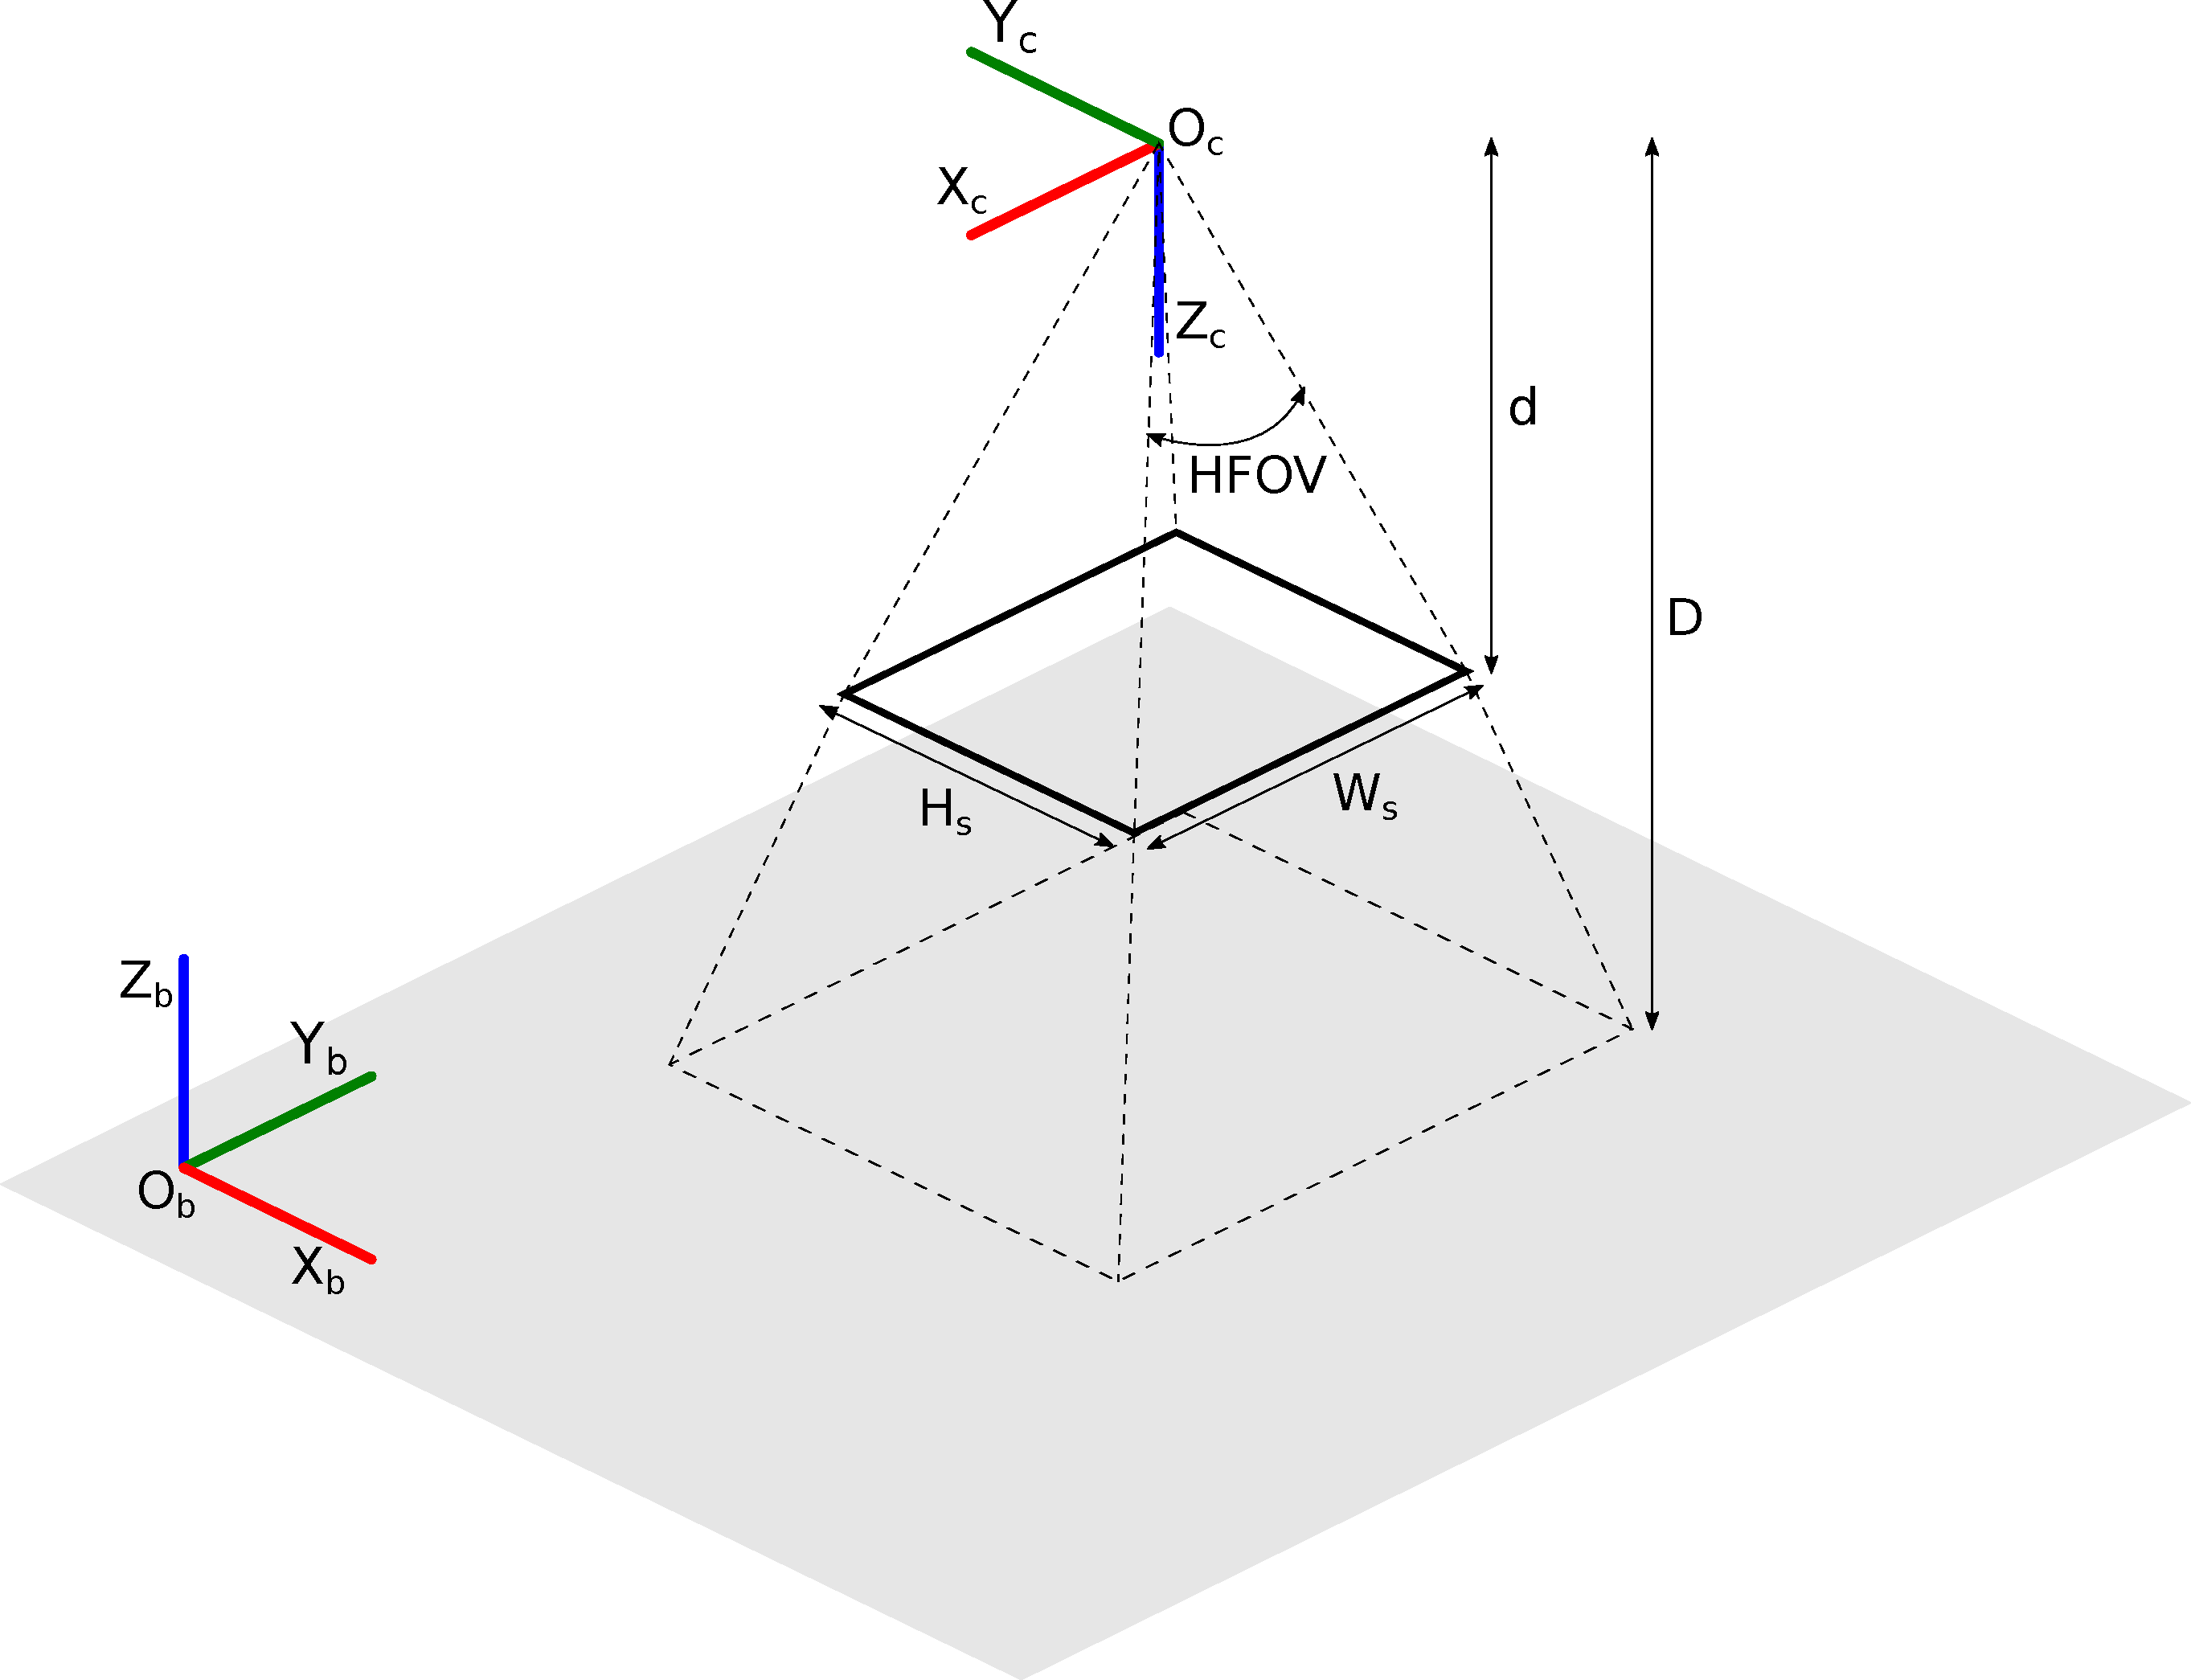
\includegraphics[width=0.6\textwidth]{system_architecture_layer_camera_spatial_data_image_wsp_dimensions}
	\caption{Width and height of the camera projected image. $W_s$ and $H_s$ represent the width and height, respectively, of the image projected from the camera at a distance $d$. In general, the camera is placed at a vertical distance $D$ from the robot base plane. $D$ and $d$ can be equal, but in general they are not.} 
	\label{fig:system_architecture_layer_camera_spatial_data_image_wsp_dimensions}
\end{figure}

According to camera specifications, at a certain resolution there is an associated \gls{hfov} in radians. By multiplying this \gls{hfov} with a distance $d$, from the camera to an object, we get the image width in meters ($W_s$). Having the width and knowing the resolution, we can easily obtain the height ($H_s$). In resume (\ref{eq:image_dimension_in_meters}),

\begin{equation}
\label{eq:image_dimension_in_meters}
    \left.
    \begin{aligned}
        r = \frac{W}{H} \\
        W_s = HFOV \times d \\
        H_s = \frac{W_s}{r} \\
    \end{aligned}
    \right.
\end{equation}

Lastly, this layer also obtains a mesh of the detected wound for possible geometrical analysis.

The mesh is obtained by intersecting the point cloud data with the image segmentation data. The point cloud data is reduced by using a box filter and point density reduction. The box filter uses $W_s$, $H_s$ and $d$ to limit x, y and z. The point density is reduced to a minimum distance between points of 5 \si{\milli \meter} in all axes (Fig. \ref{fig:system_architecture_layer_camera_spatial_data_mesh_generation}). All the pixels inside the wound contour are selected and converted to the robot base frame (\ref{eq:camera_point_transform_robot_base_camera}). Afterwards, these points are used to filter the point cloud 3D points to select only the desired region (Fig. \ref{fig:system_architecture_layer_camera_spatial_data_mesh_generation}).

After the point cloud data is filtered, an algorithm is applied to calculate the surface normals and mesh triangulation. The final result is stored in file, using the \textbf{Polygon File Format} or \textbf{Stanford Triangle Format}. This file format uses the extension \textbf{ply}.

\begin{figure}[htbp]
	\centering
	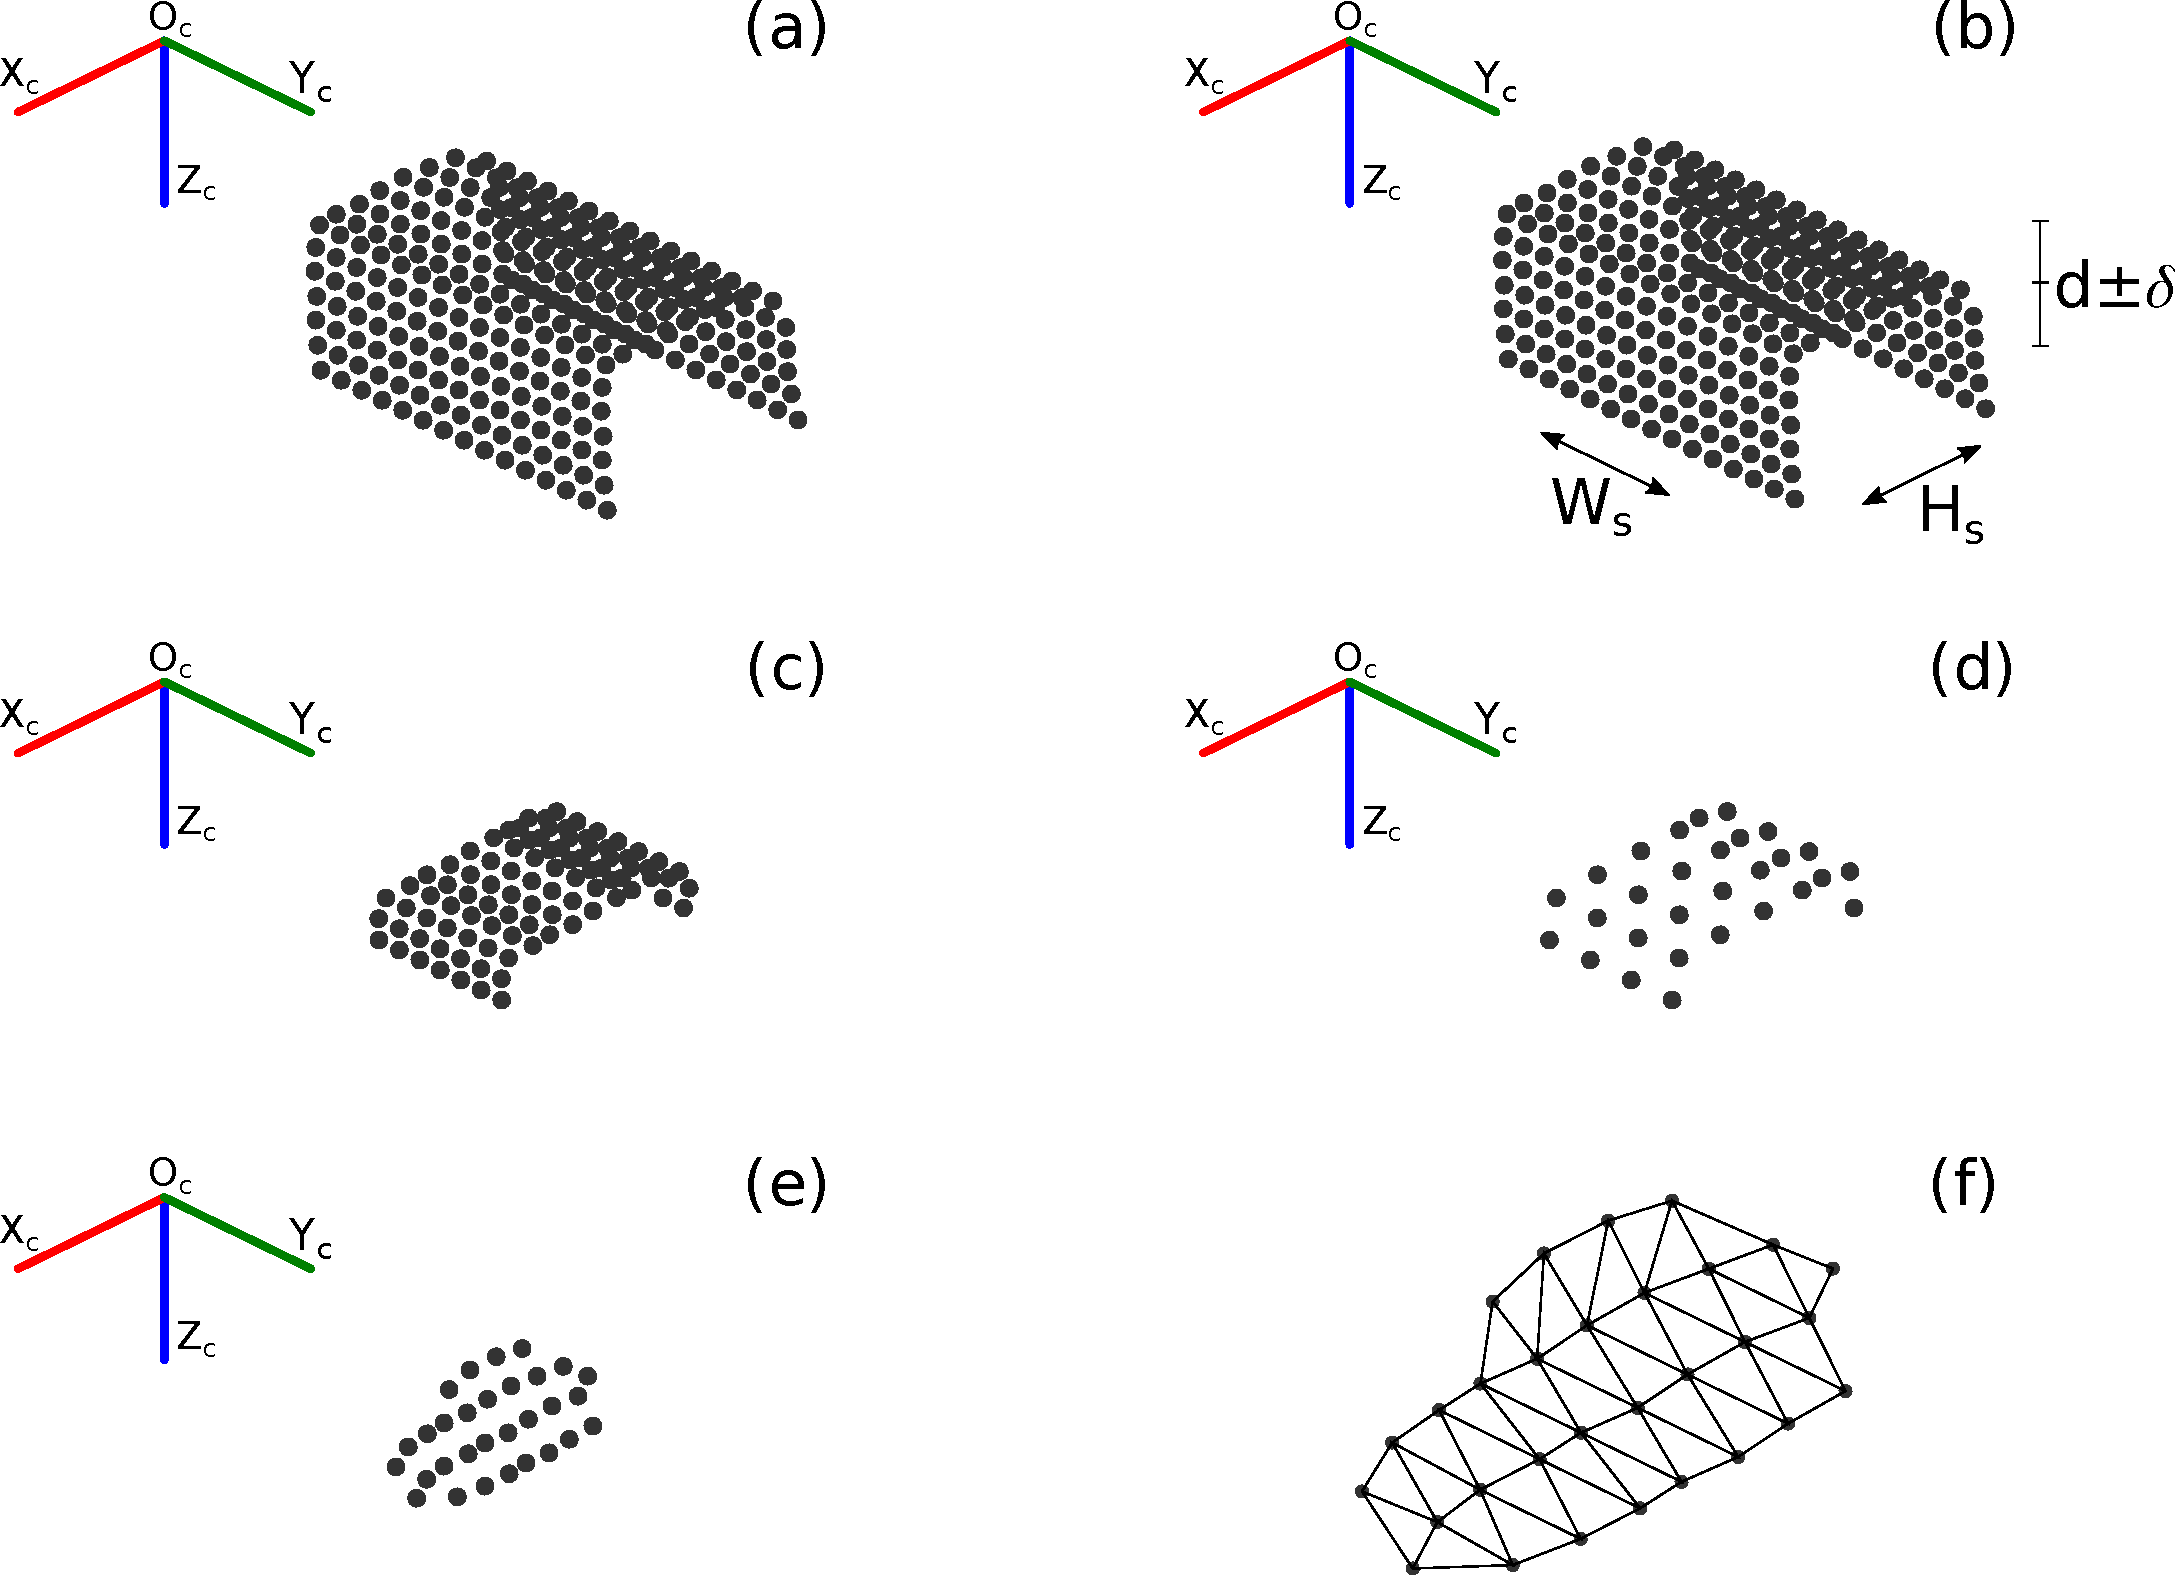
\includegraphics[width=0.6\textwidth]{system_architecture_layer_camera_spatial_data_mesh_generation}
	\caption{Mesh generation procedure. (a) The point cloud data of the wound area is obtained. (b) The $W_s$, $H_s$ and $d$ dimensions are used to limit the point cloud points to the wound location volume. (c) After applying the volume filter a simplified point cloud is obtained. (d) The point cloud data is reduced further by establishing a minimum distance between points. (e) After fully simplifying the point cloud, only the points that match the wound position are selected to generate the final wound point cloud. (f) With the previous data a wound mesh is generated. }
	\label{fig:system_architecture_layer_camera_spatial_data_mesh_generation}
\end{figure}

% subsubsection system_architectural_camera_layers_spatial_data

% subsection system_architectural_camera_layers

\subsection{Robot Layers}
\label{subsec:system_architectural_robot_layers}

The robot layers deal with the control of the robotic arm to execute the wound filling bioprinting.

\subsubsection*{Spatial Data Processing}
\label{subsubsec:system_architectural_robot_layers_spatial_data}

This layer, which seems to duplicate the layer with the same name from the camera layers, exists for the cases of co-manipulation. 

When using co-manipulation, the operator is responsible for detecting and segmenting the wound using the robotic arm. This layer also gathers position, calculates wound area, perimeter and mesh. Figure \ref{fig:system_architecture_layer_robot_spatial_data_flowchart} presents the flowcharts for robot spatial data processing.

\begin{figure}[htbp]
	\centering
	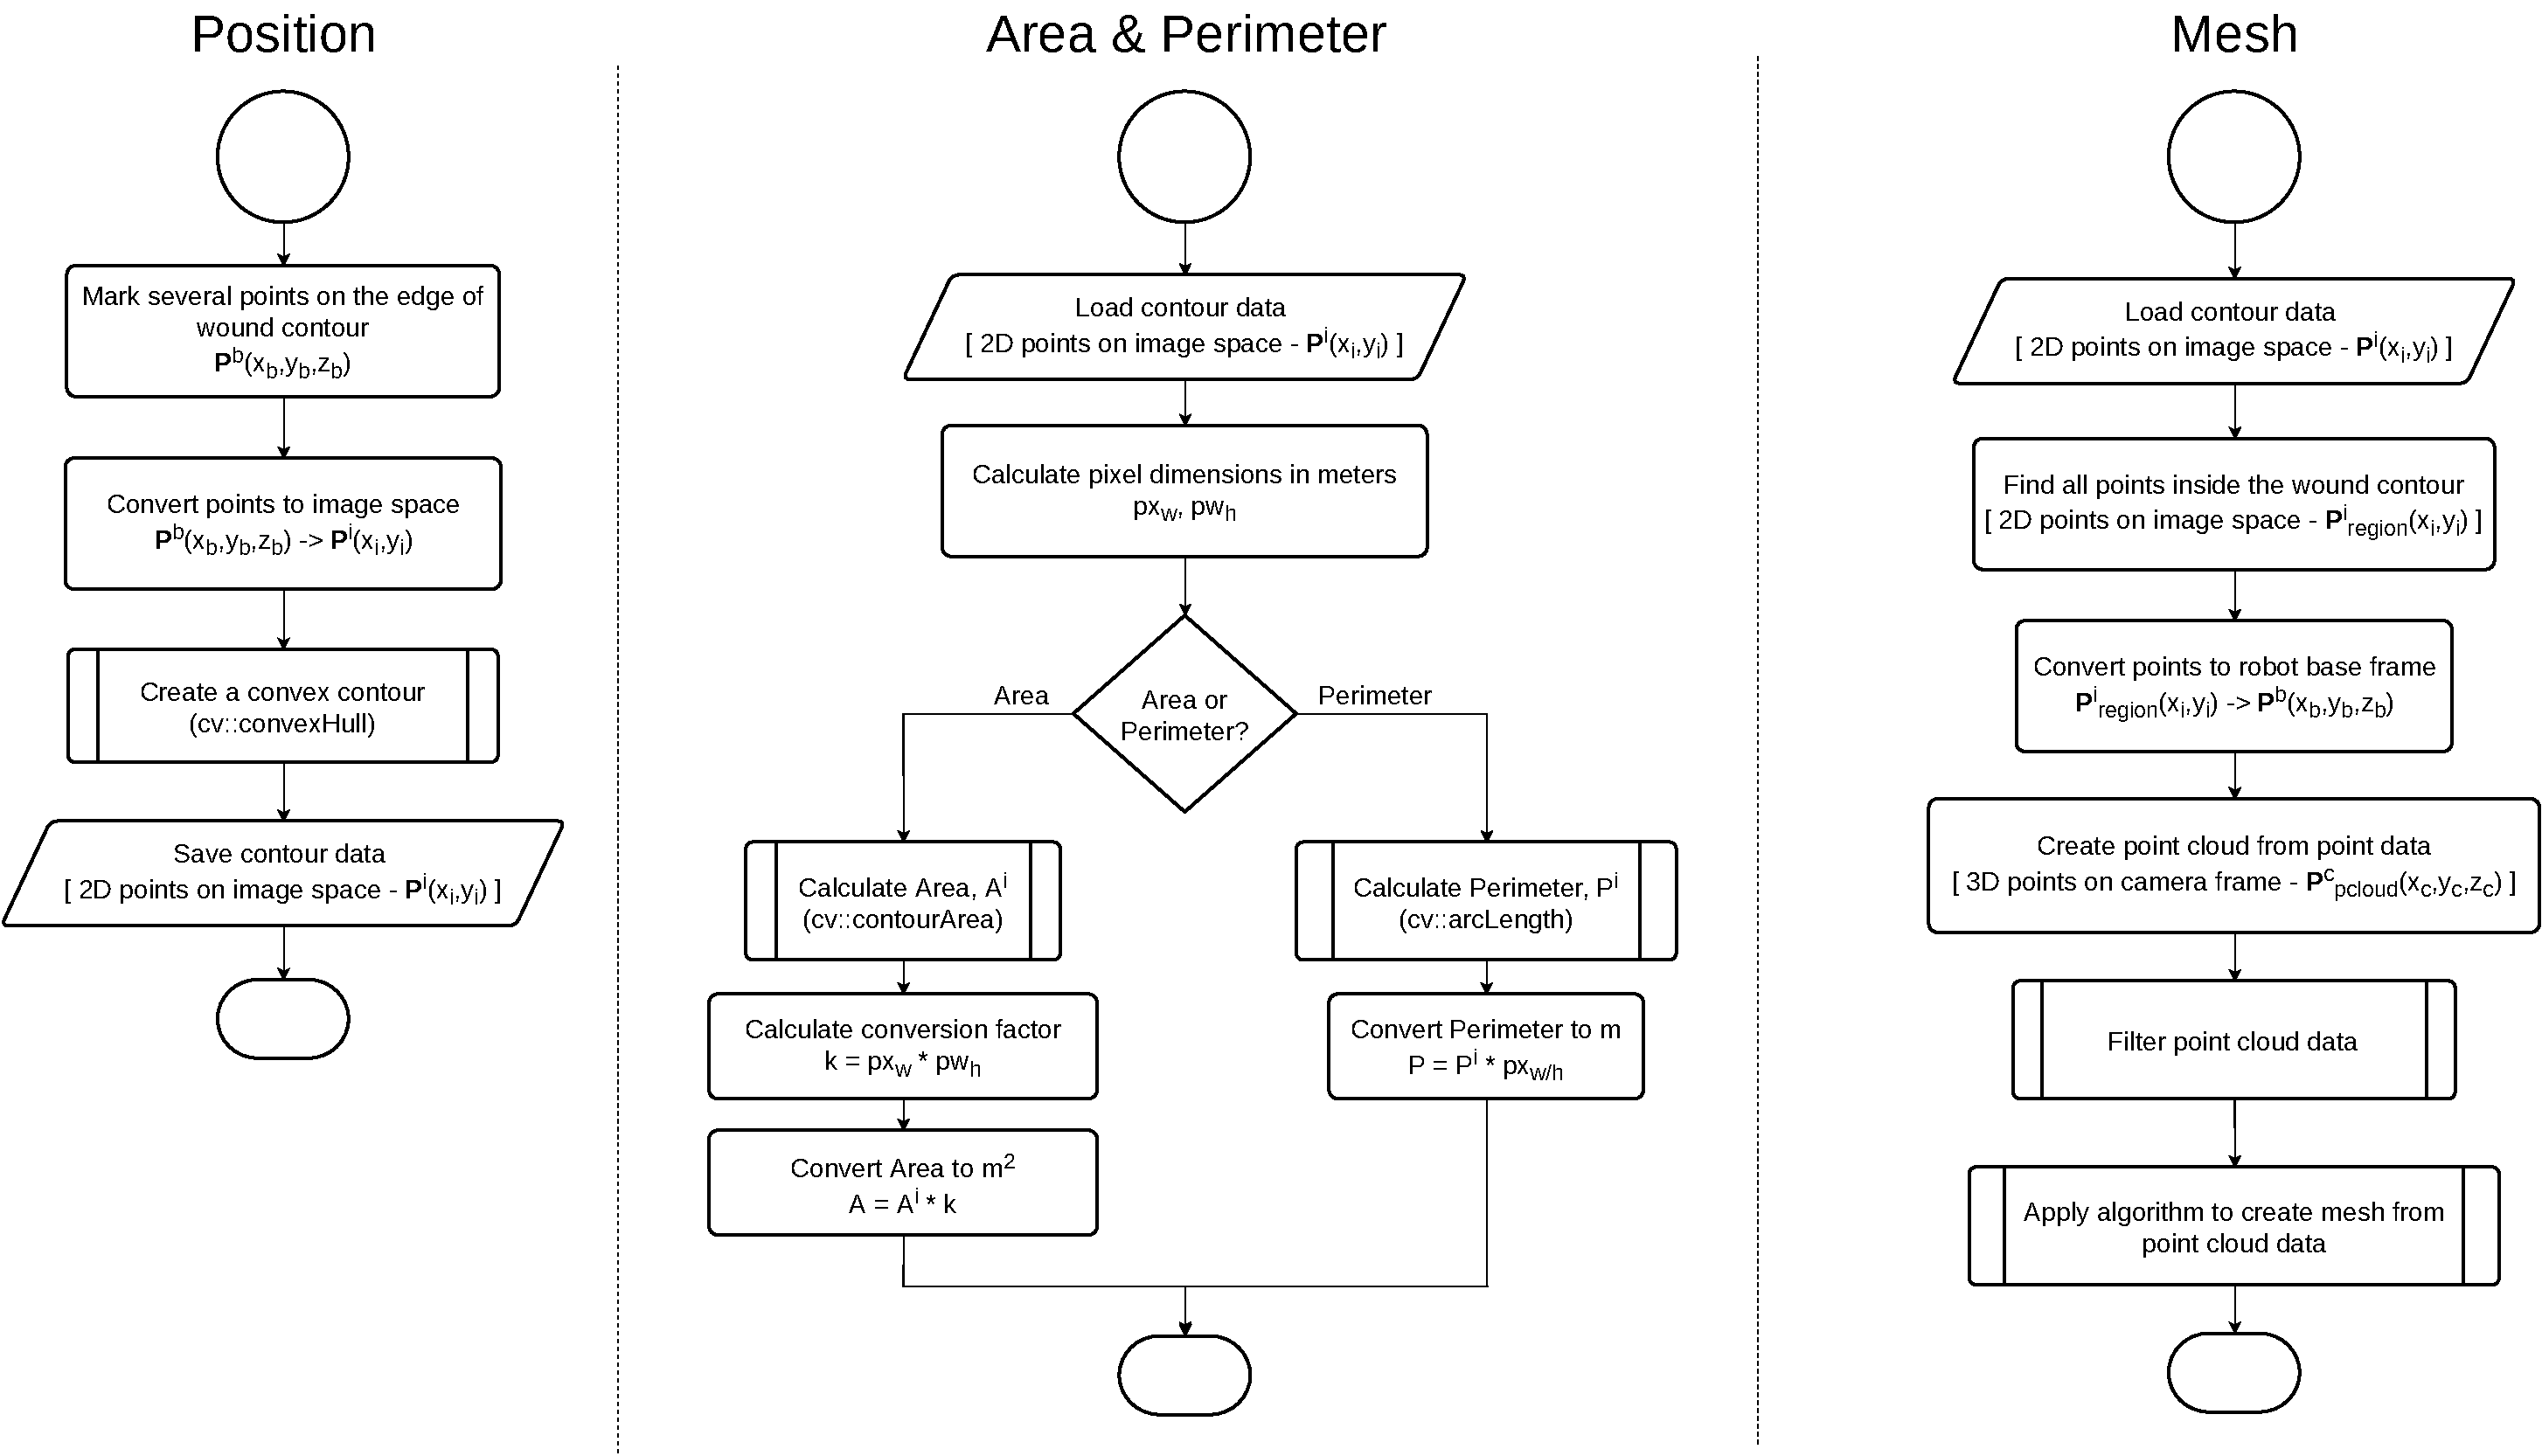
\includegraphics[width=\textwidth]{system_architecture_layer_robot_spatial_data_flowchart}
	\caption{Robot spatial data processing flowcharts. At the left, the flowchart for obtaining wound position. In the middle, the flowchart to calculate the wound area and perimeter. At the right, mesh generation flowchart. Refer to appendix \ref{app:architectural_layers_flowcharts} for full size images.}
	\label{fig:system_architecture_layer_robot_spatial_data_flowchart}
\end{figure}

The position is obtained through co-manipulation and it is already referenced to the robot base frame, which means it does not need any transformations.

The operator moves the robot to the desired points which define the wound contour and marks them. After all the points are marked and stored, they are converted to image space (Fig. \ref{fig:system_architecture_layer_robot_spatial_data_frame_conversions}) to create a convex contour. Later, they are used to calculate the other features.\\

To calculate the wound area and perimeter, the image space is used again. This approach was followed because the algorithms were already developed on this space. A new transformation is needed.

The transformation approach used was to establish a relation between the robot base frame x-y plane and the image x-y frame (Fig. \ref{fig:system_architecture_layer_robot_spatial_data_frame_conversions}).

\begin{figure}[htbp]
	\centering
	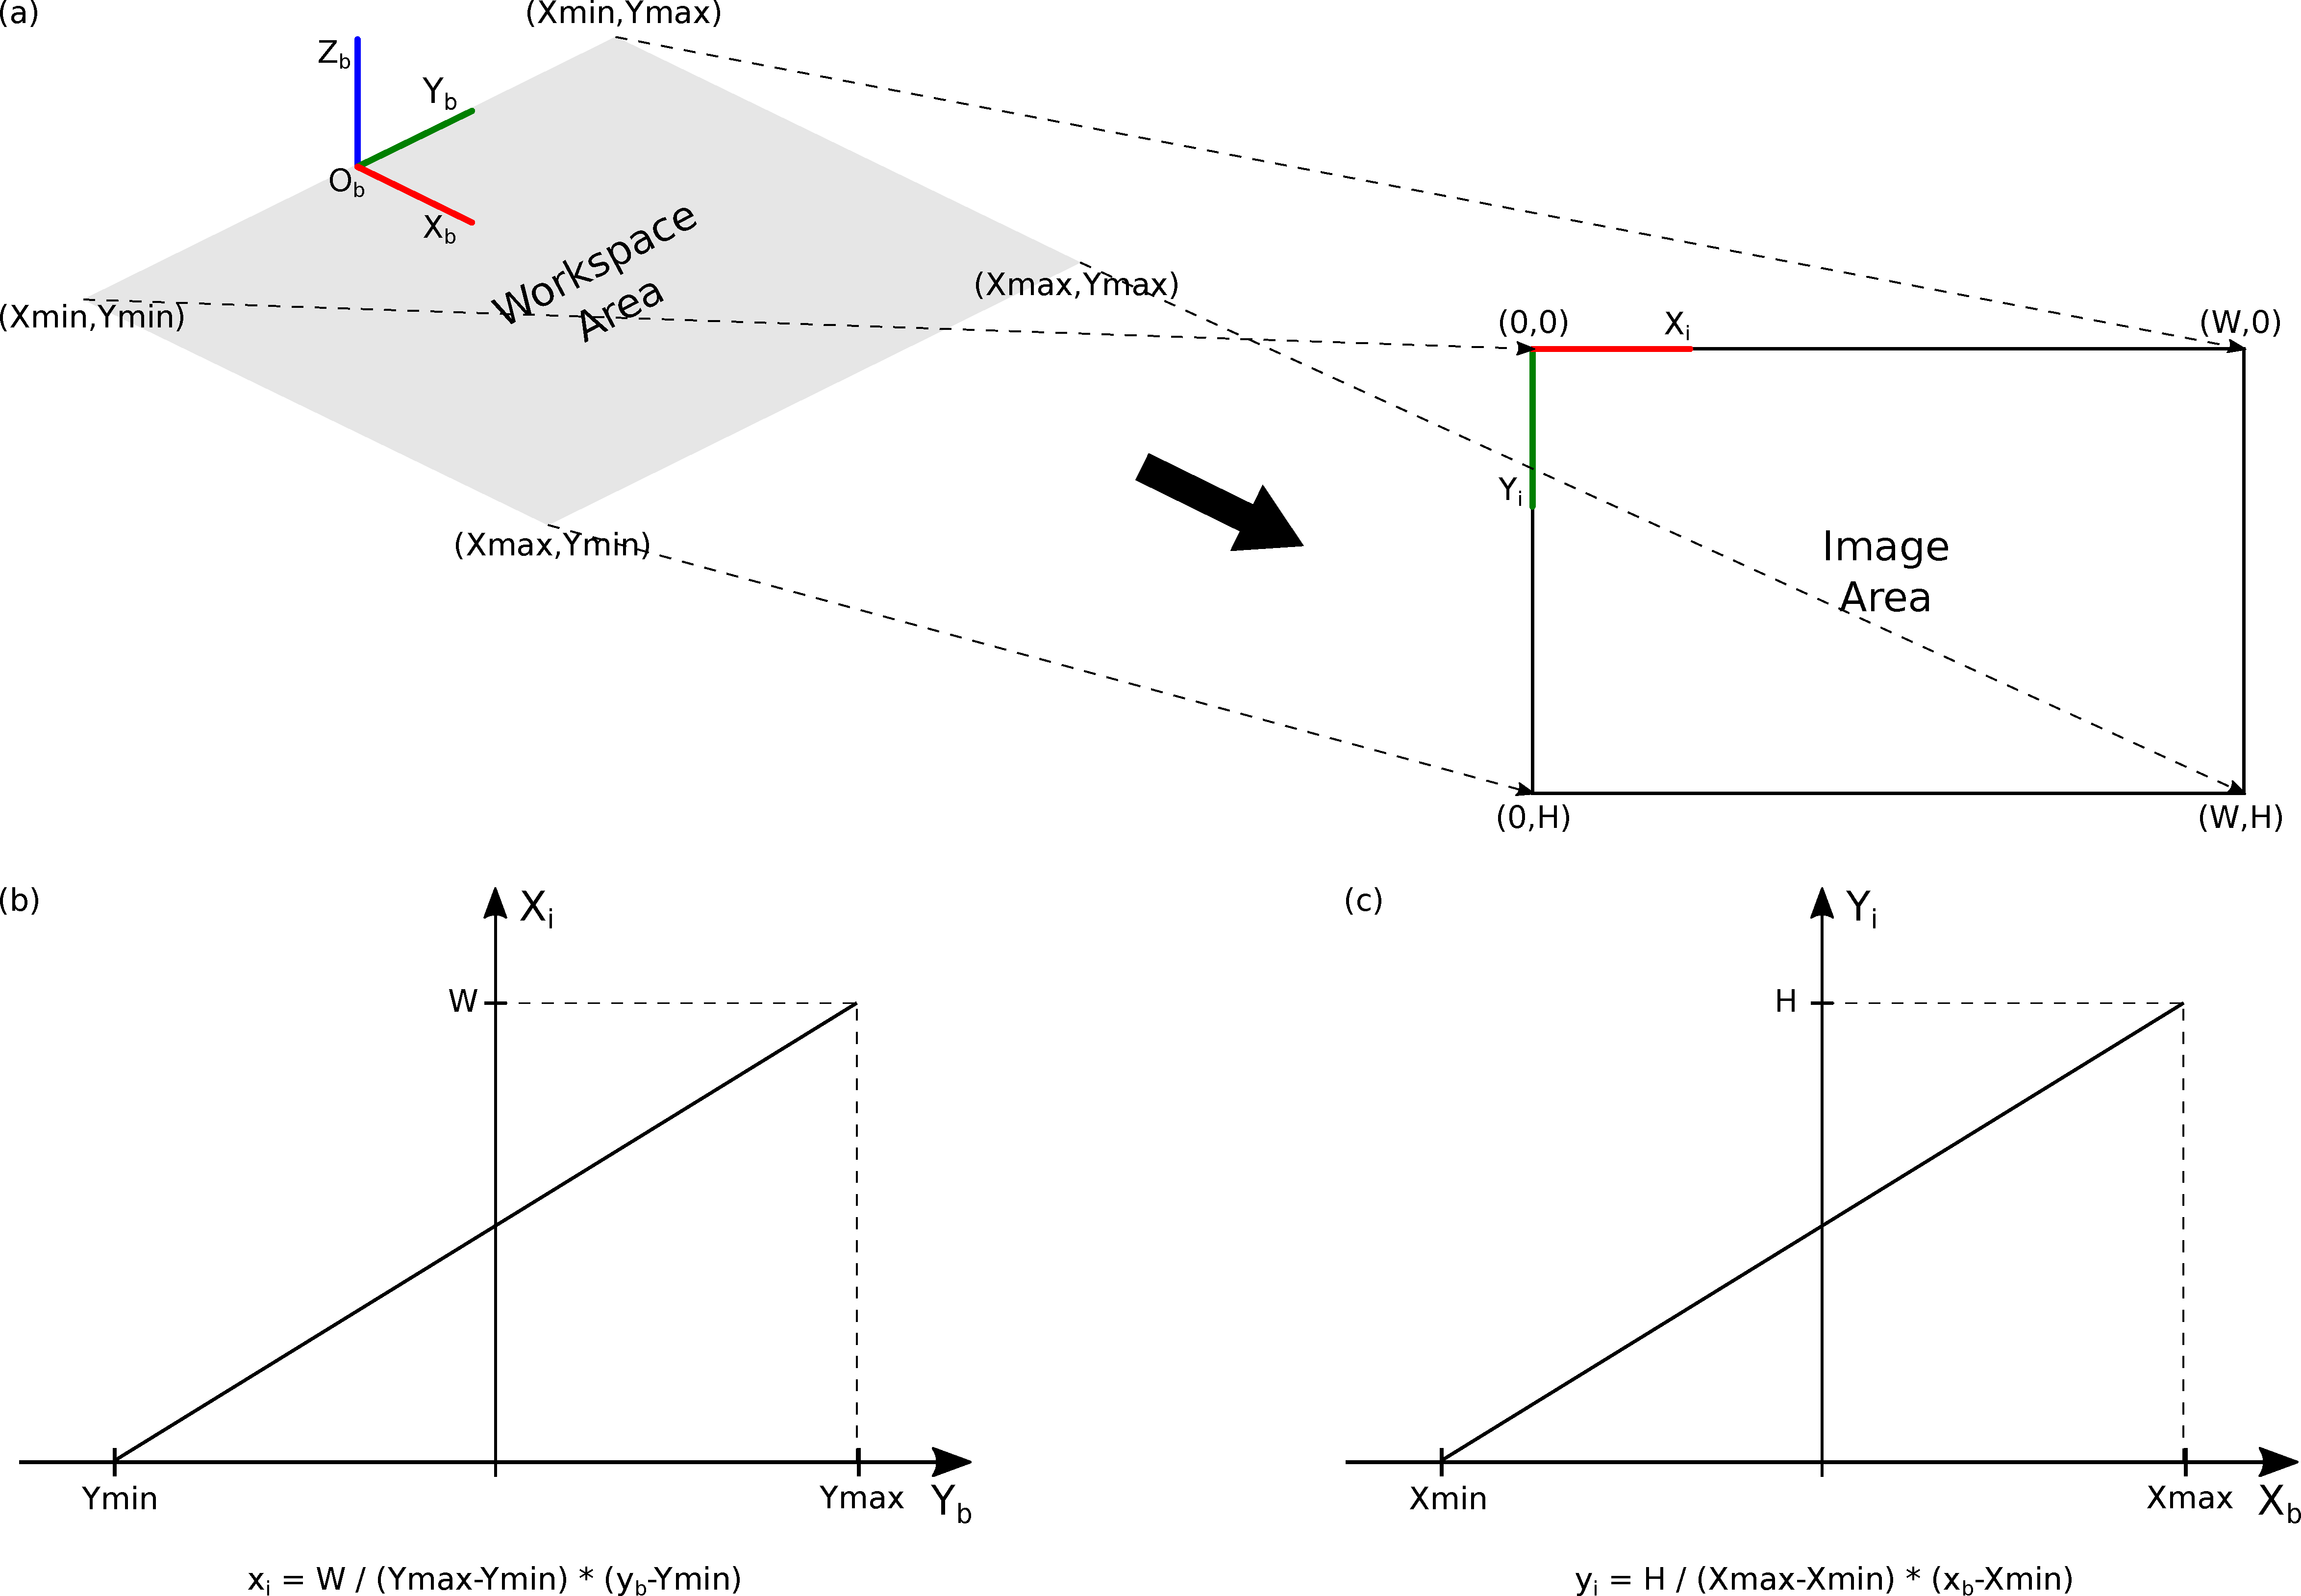
\includegraphics[width=\textwidth]{system_architecture_layer_robot_spatial_data_frame_conversions}
	\caption{Transformation between robot base frame x-y plane and image x-y frame. (a) Coordinates relation overview between both frames. (b) Conversion formula to obtain $x_i$ coordinate. (c) Conversion formula to obtain $y_i$ coordinate.}
	\label{fig:system_architecture_layer_robot_spatial_data_frame_conversions}
\end{figure}

The conversion between robot base coordinates and image coordinates are presented on equations \ref{eq:convert_y_robot_x_image} and \ref{eq:convert_x_robot_y_image},

\begin{equation}
\label{eq:convert_y_robot_x_image}
    x_i = \frac{W}{Y_{max} - Y_{min}} \times (y_b - Y_{min})
\end{equation}

\begin{equation}
\label{eq:convert_x_robot_y_image}
    y_i = \frac{H}{X_{max} - X_{min}} \times (x_b - X_{min})
\end{equation}

where, ($x_i, y_i$) represent the image coordinates and ($x_b, y_b$) the robot base coordinates. $Y_{min/max}$ and $X_{min/max}$ are the robot workspace limits on the x-y plane. They can be defined by the robot physical limits or by the task-defined limits. $W$ and $H$ are the image width and height, respectively. They can be arbitrarily chosen, although optimal values exist that minimise the errors when converting the area and perimeter to \si{\meter \squared} and \si{\meter}, respectively. These optimal values were not calculated.

With all the points converted to the image space, the area and perimeter algorithms are applied to calculate the desired quantities.\\

Regarding the calculation of the mesh, it was not possible to obtain a valid mesh from the data acquired. The algorithm for mesh creation needs a point cloud structure, which we do not have in this case.

For a planar wound, it was possible to define a custom point grid inside the wound profile and create a point cloud from it. With this point cloud it would be possible to generate a mesh. However, the main goal of having a mesh is to extract geometrical information from a non-planar surface, which consists on the majority of human wound profiles. Although several approaches were tried, none was successful.

% subsubsection system_architectural_robot_layers_spatial_data

\subsubsection*{Path Planning}
\label{subsubsec:system_architectural_robot_layers_path_planning}

The path planning layer is responsible for defining a valid wound filling path. There exist many possible paths for wound filling. This work uses three different paths derived from the same base algorithm. This algorithm is inspired on \cite{Ding2018_simulated_insitu_bioprinting_wound_bed_path_planning}. The paths are called \gls{zz}, \gls{pl} and \gls{gd}. Figure \ref{fig:system_architecture_layer_robot_path_flowchart} presents the flowchart of path planning.

\begin{figure}[htbp]
	\centering
	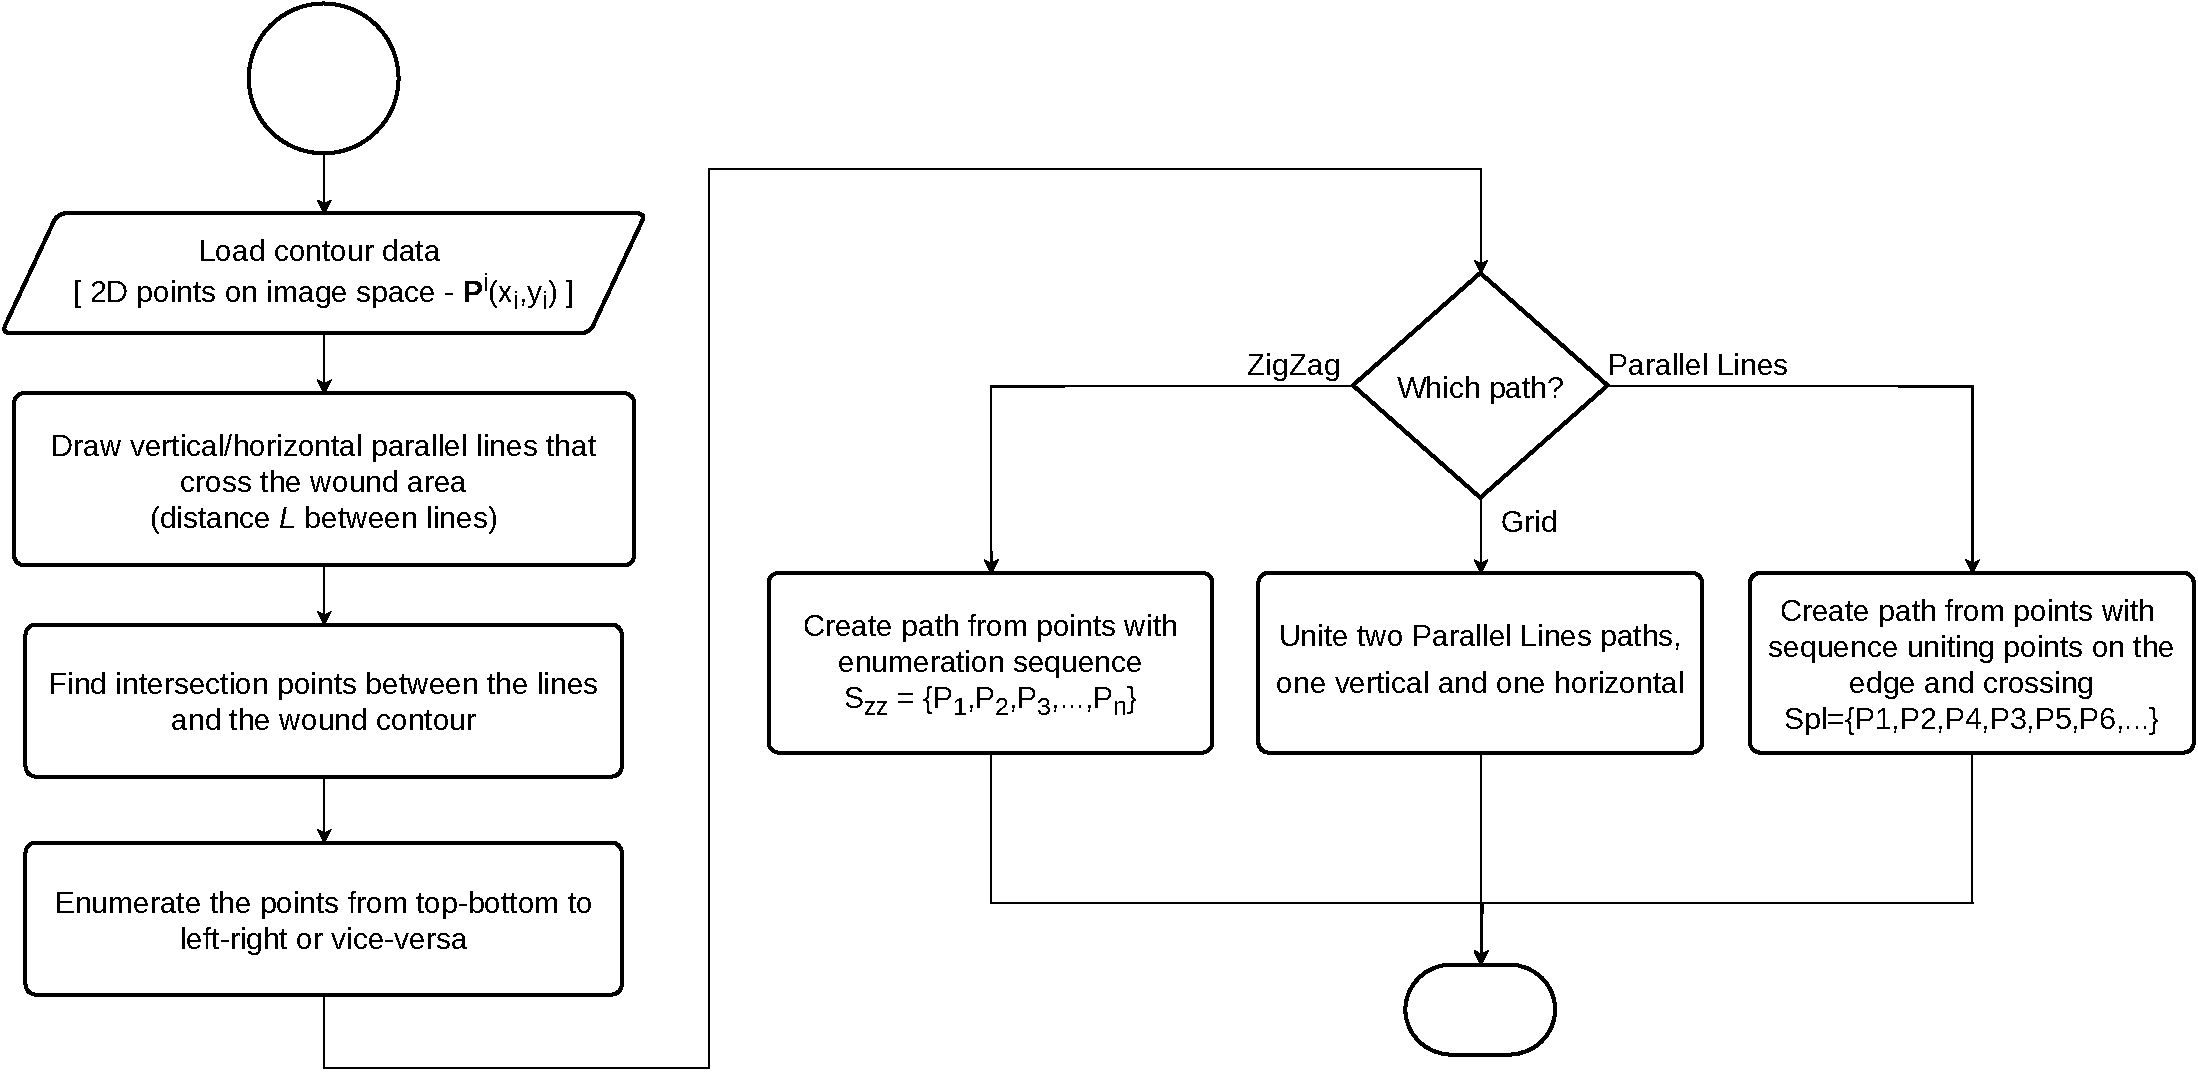
\includegraphics[width=\textwidth]{system_architecture_layer_robot_path_flowchart}
	\caption{Robot path planning flowchart. All three paths use the same base algorithm to find the path points. Each path differentiate on the way the path points are ordered.}
	\label{fig:system_architecture_layer_robot_path_flowchart}
\end{figure}

The base algorithm, applied on the image space, consists on the following steps (see also Fig. \ref{fig:system_architecture_layer_robot_path_planning_base_algorithm}a):

\begin{enumerate}
    \item Obtain the wound contour (supplied by previous layer).
    \item Draw parallel lines, at a certain distance $L$ from each other, that extend beyond the wound contour. They can be parallel to the x axis or y axis.
    \item Find the intersection points between the lines and the contour.
    \item The points are numerated from top to bottom and left to right in case of lines parallel to y axis, or left to right and top to bottom otherwise.
\end{enumerate}

\begin{figure}[htbp]
	\centering
	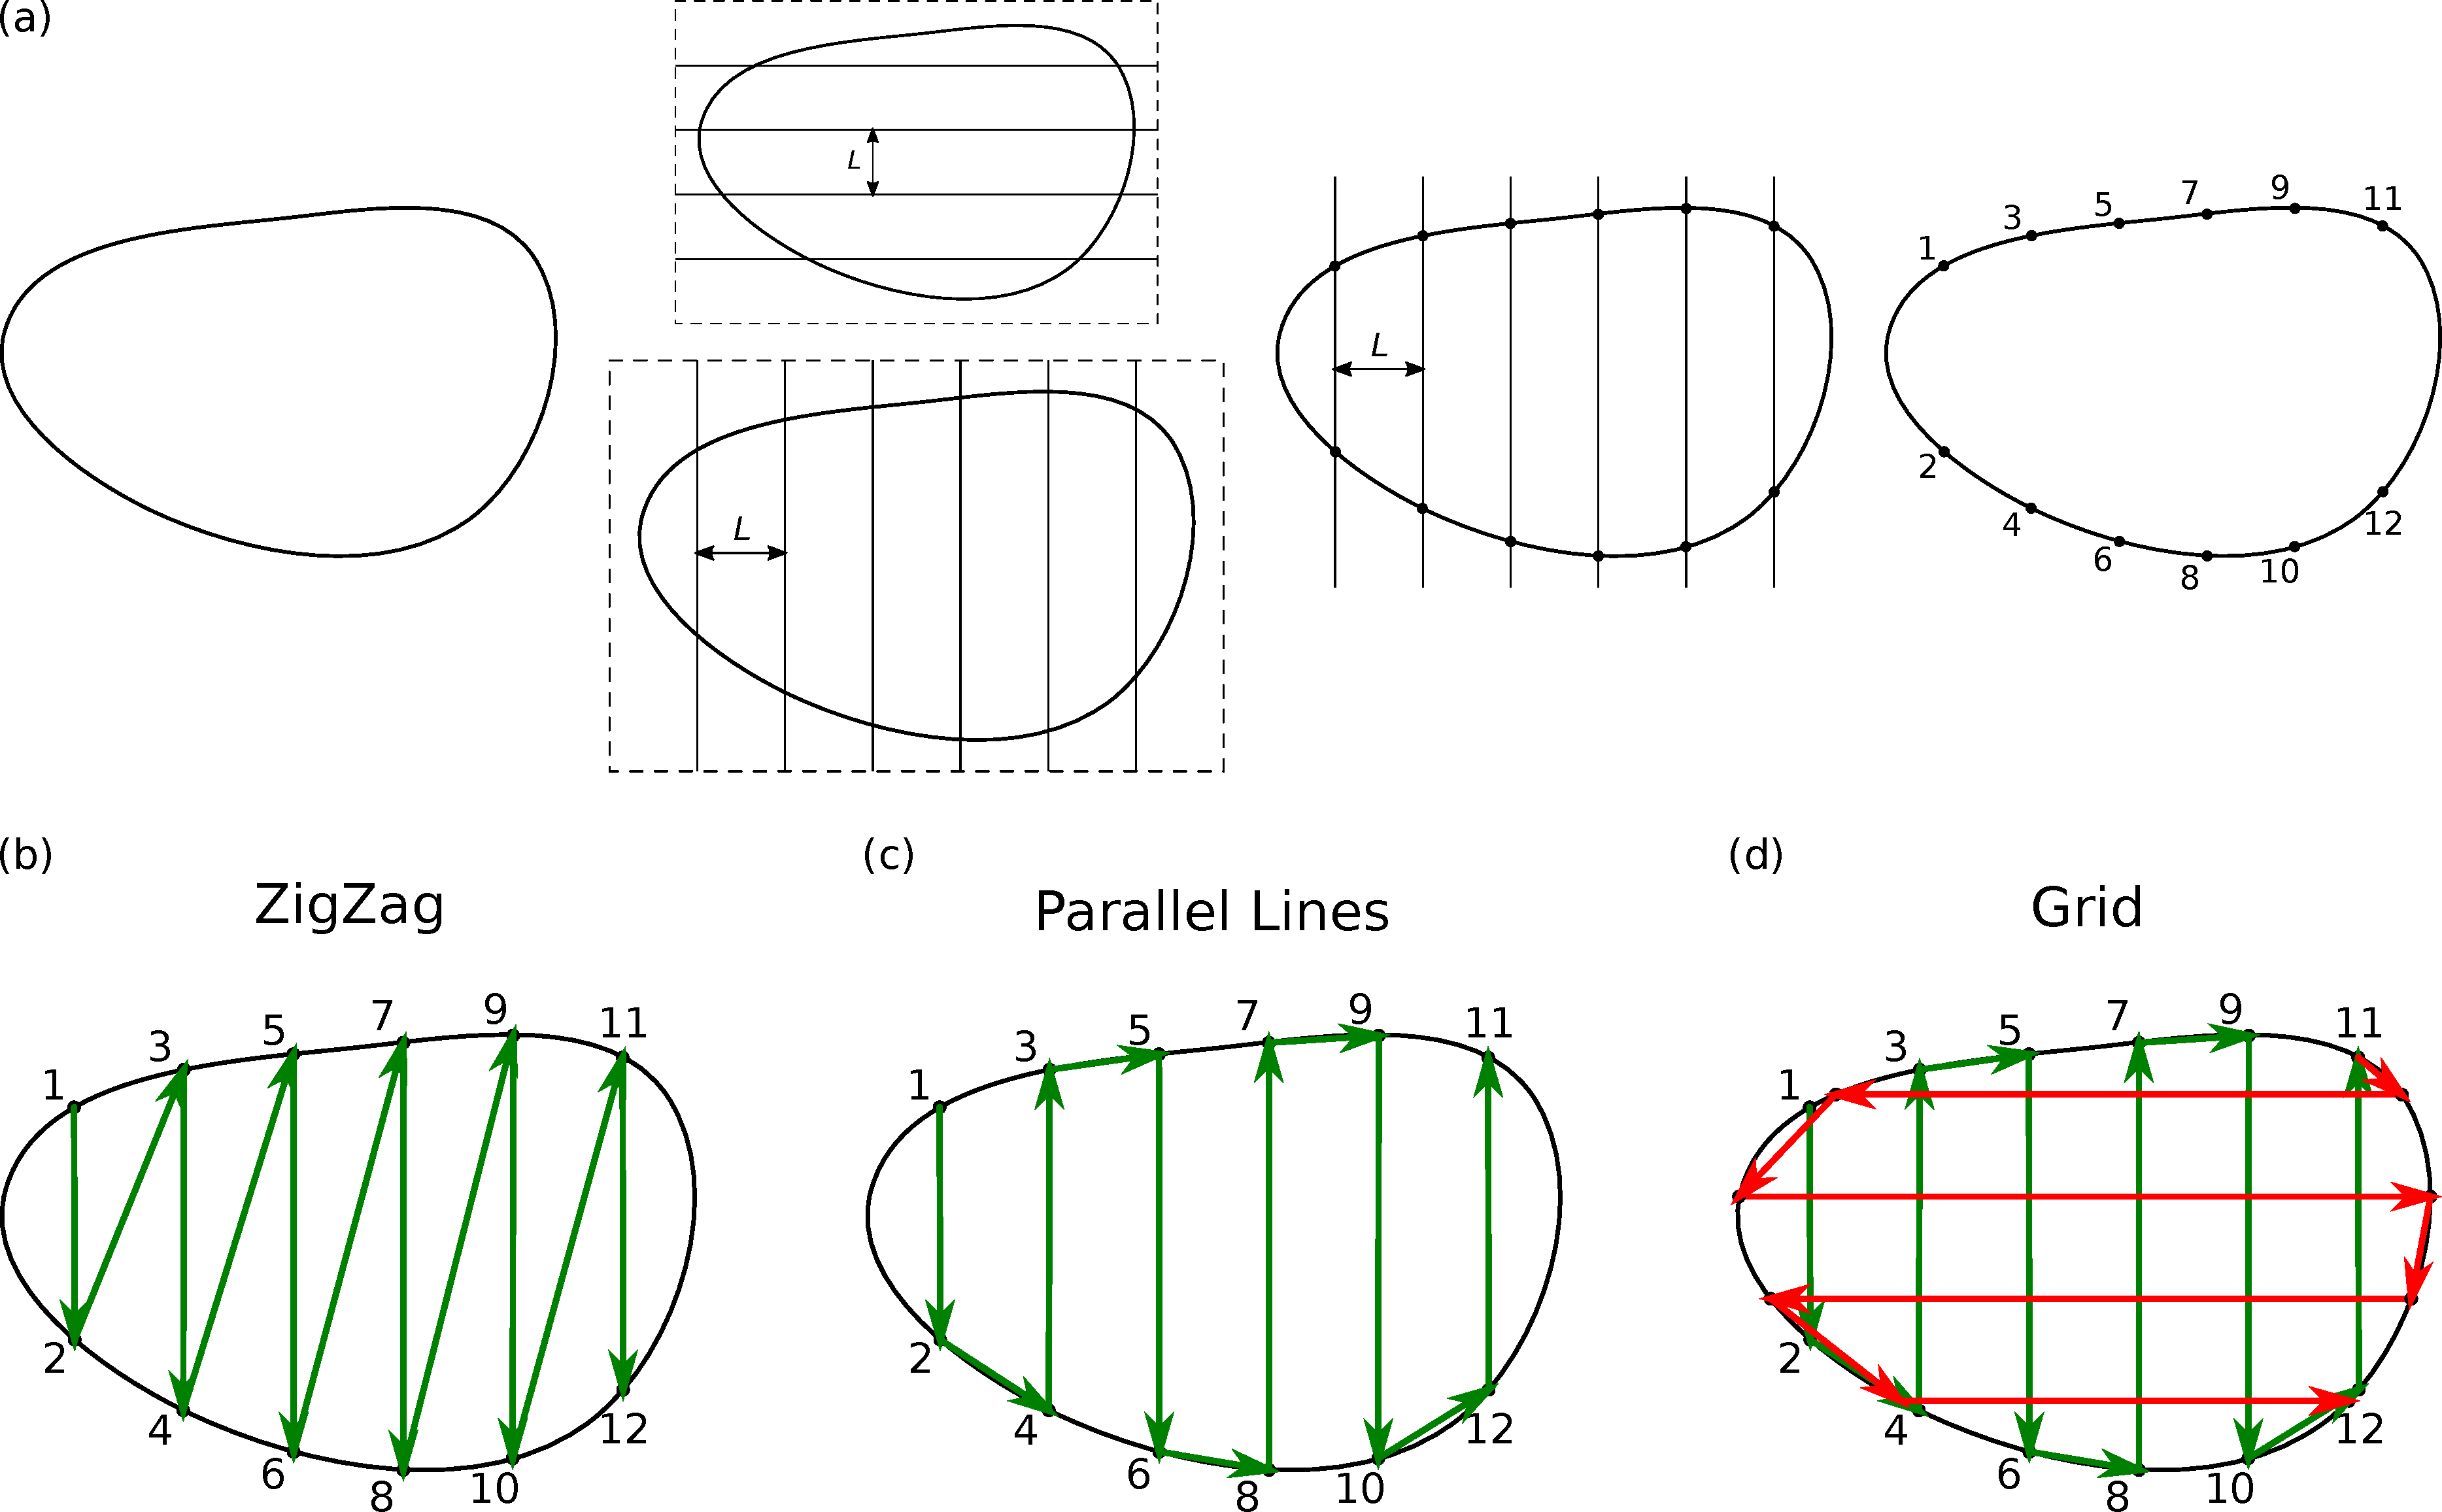
\includegraphics[width=\textwidth]{system_architecture_layer_robot_path_planning_base_algorithm}
	\caption{Robot path planning algorithms. (a) Shows the 4 steps of the path planning base algorithm from which all paths derive. Steps follow from left to right. (b) ZigZag path planning sequence. (c) Parallel Lines path planning sequence. (d) Grid path planning sequence.}
	\label{fig:system_architecture_layer_robot_path_planning_base_algorithm}
\end{figure}

Now, having these points defined, each path is derived from the sequence connecting the points. It is the order in which these points are organised in a set that defines the path.\\

The ZigZag path's set follows exactly the sequence in which the points were obtained (\ref{eq:zigzag_path_set}),

\begin{equation}
\label{eq:zigzag_path_set}
    S_{WFP} = S_{zz} = \{ P_1, P_2, P_3, ..., P_n \}
\end{equation}

where $n$ is the number of points (see Fig. \ref{fig:system_architecture_layer_robot_path_planning_base_algorithm}b).\\

The Parallel Lines path's set ordering is more complex. In this case, the goal is for that path to run along the contour after crossing it. If the lines are parallel to the y axis, points $P_1$ and $P_3$ would be at the top and $P_2$ and $P_4$ at the bottom. The sequence would be, $\{P_1, P_2, P_4, P_3, ...\}$ (\ref{eq:parallel_lines_path_set}). This is so because points $P_1$ and $P_2$ define the first crossing line. After that, the path should follow along the contour, i.e., uniting points $P_2$ and $P_4$ at the bottom. After that, it does another crossing connecting points $P_4$ and $P_3$ (see Fig. \ref{fig:system_architecture_layer_robot_path_planning_base_algorithm}c).

\begin{equation}
\label{eq:parallel_lines_path_set}
    S_{WFP} = S_{pl} = \{ P_1, P_2, P_4, P_3, P_5, P_6, P_8, P_7, P_9, ... \}
\end{equation}

The Grid path is basically the Parallel Lines path duplicated, using first lines parallel to the x axis and afterwards to the y axis. The second path uses reverse ordering so that the first point stays closer to the last point of the first path (see Fig. \ref{fig:system_architecture_layer_robot_path_planning_base_algorithm}d).\\

After the path is calculated on the image space, the points are converted to the robot base frame as poses. The poses have x, y, and z coordinates for the position. The way to obtain the three coordinates from the image will depend if the system is using the camera or working via co-manipulation.\\

When using the camera the following algorithm is used:

\begin{enumerate}
    \item Convert the path points to camera frame with $z = d$ (Fig. \ref{fig:system_architecture_layer_camera_spatial_data_image_wsp_dimensions}), $\boldsymbol{P}^c_{path}(x_c, y_c, z_c)$.
    \item Convert the points from path to the robot base frame using equation \ref{eq:camera_point_transform_robot_base_camera}, $\boldsymbol{P}^b_{path}(x_b, y_b, z_b)$.
    \item For each $\boldsymbol{P}^b_{path}$ point, search for a $\boldsymbol{P}^b_{region}$ point that is within a small range of the path point (\ref{eq:point_conversion_valid_range}).
    \item For all the points that match, store the region point as a path pose. The orientation used is vertical, with end-effector pointing down.
\end{enumerate}

When doing co-manipulation the following algorithm is used:

\begin{enumerate}
    \item Based on the parameters used for converting the points from robot base to image coordinates, calculate the pixel dimensions, $px_w$ and $px_h$.
    \item For each path point, convert the $x_i$ and $y_i$ coordinates to robot base coordinates, $x_b$ and $y_b$, using (\ref{eq:convert_image_to_robot_base_x}, \ref{eq:convert_image_to_robot_base_y})
    \item Add a user defined z coordinate that will establish an offset between the print head and the wound surface. Store points as path poses with vertical orientation, end-effector pointing down.
\end{enumerate}

\begin{equation}
\label{eq:convert_image_to_robot_base_x}
    x_b = X_{min} + (y_i \times px_w)
\end{equation}
\begin{equation}
\label{eq:convert_image_to_robot_base_y}
    y_b = Y_{min} + (x_i \times px_h)
\end{equation}

% subsubsection system_architectural_robot_layers_path_planning

\subsubsection*{Trajectory Definition}
\label{subsubsec:system_architectural_robot_layers_trajectory_definition}

On this layer, the wound filling path is converted to a trajectory, i.e., the path has an execution time, speed and acceleration defined. Besides, the movement of the robot arm to the start pose of the wound filling path is also taken into account. Added to the data of each pose, is a printing command, which will instruct the bioprinting system when to start/stop dispensing the bioink. Figure \ref{fig:system_architecture_layer_robot_trajectory_flowchart} presents the flowchart of trajectory definition.

\begin{figure}[htbp]
	\centering
	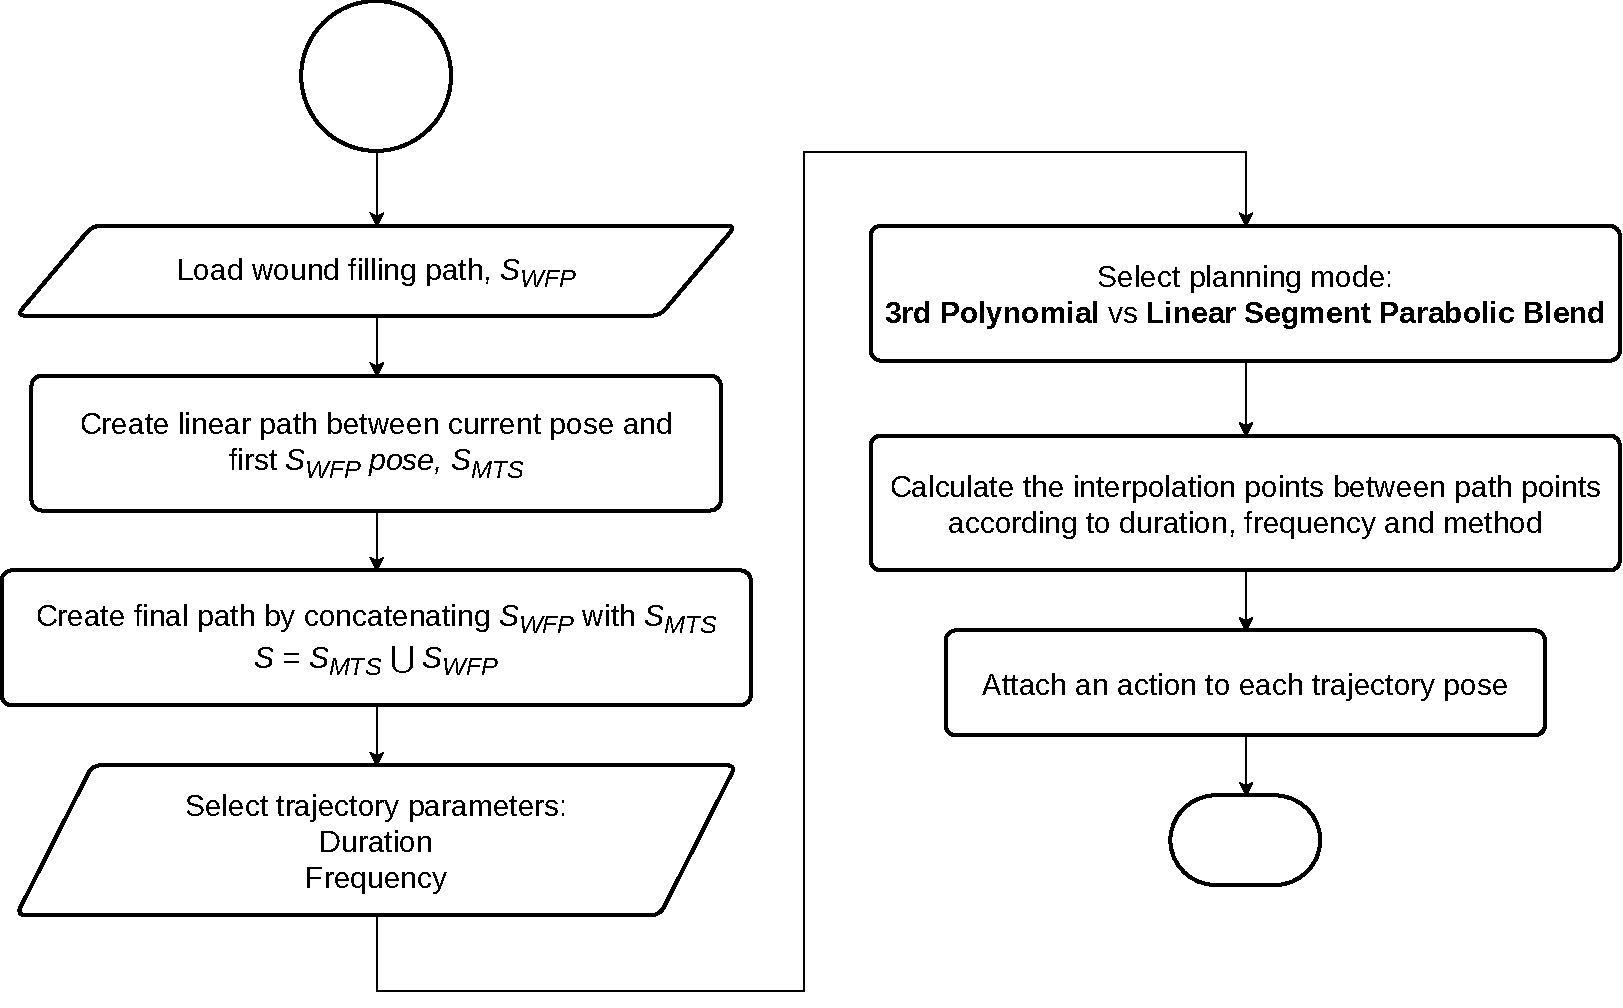
\includegraphics[width=\textwidth]{system_architecture_layer_robot_trajectory_flowchart}
	\caption{Robot trajectory definition flowchart.}
	\label{fig:system_architecture_layer_robot_trajectory_flowchart}
\end{figure}

The trajectory is defined by concatenating two paths, $S_{MTS}$, which is the movement from current pose to the start of the wound filling path pose, and $S_{WFP}$, the wound filling path itself.

The $S_{MTS}$ is, on the simplest approach, a linear path uniting two poses. Other more complicated paths can be used depending on the task restrictions, e.g., to avoid obstacles.\\

The approach used to calculate the trajectories is based on defining a trajectory duration and frequency, and derive the speed and acceleration from it. Two algorithms were used, a $3^{rd}$ order polynomial and \gls{lspb}. The technical details of these algorithms are defined on subsection \ref{subsec:path_trajectory_planning}.

What both algorithms do is to generate intermediate poses between the path points, by interpolation, to create a smooth movement between path poses. The number of intermediate points will depend on the trajectory duration, $t$, and the robot arm control frequency, $f$. Since each new pose is sent to the robot at the control frequency, the right trajectory duration will only be obtained by creating $n$ intermediate points, calculated using equation \ref{eq:n_intermediate_trajectory_points}, 

\begin{equation}
\label{eq:n_intermediate_trajectory_points}
    n = (\frac{t}{N-1} \times f) - 2
\end{equation}

with $t$ in seconds, $f$ in \si{\hertz} and $N$ the total number of path poses.\\

The printing commands defined are START, STOP and CONTINUE. As the names imply, the START/STOP commands are annexed to a point when the printing should start/stop. The CONTINUE is used on all the points between the start and stop. The START and CONTINUE commands imply bioink dispensing. The STOP command is to stop dispensing.

% subsubsection system_architectural_robot_layers_trajectory_definition

\subsubsection*{Visual Servoing \& Control}
\label{subsubsec:system_architectural_robot_layers_visual_servoing_control}

The Visual Servoing \& Control layer is the one executing the robot arm control algorithms. Without this layer it is not possible to control the robot arm. It receives the robot trajectory, or more specifically, the next pose to where the robot should move. The trajectory execution is basically the continuous sending of new poses to the robot arm control.

The responsibility of the robot arm control algorithms is to execute a control loop that sends binaries to the robot motors and guarantees that the robot changes to the correct desired pose and stays there. Figure \ref{fig:system_architecture_layer_robot_control_flowchart} will present a simplified overview flowchart of this layer.

\begin{figure}[htbp]
	\centering
	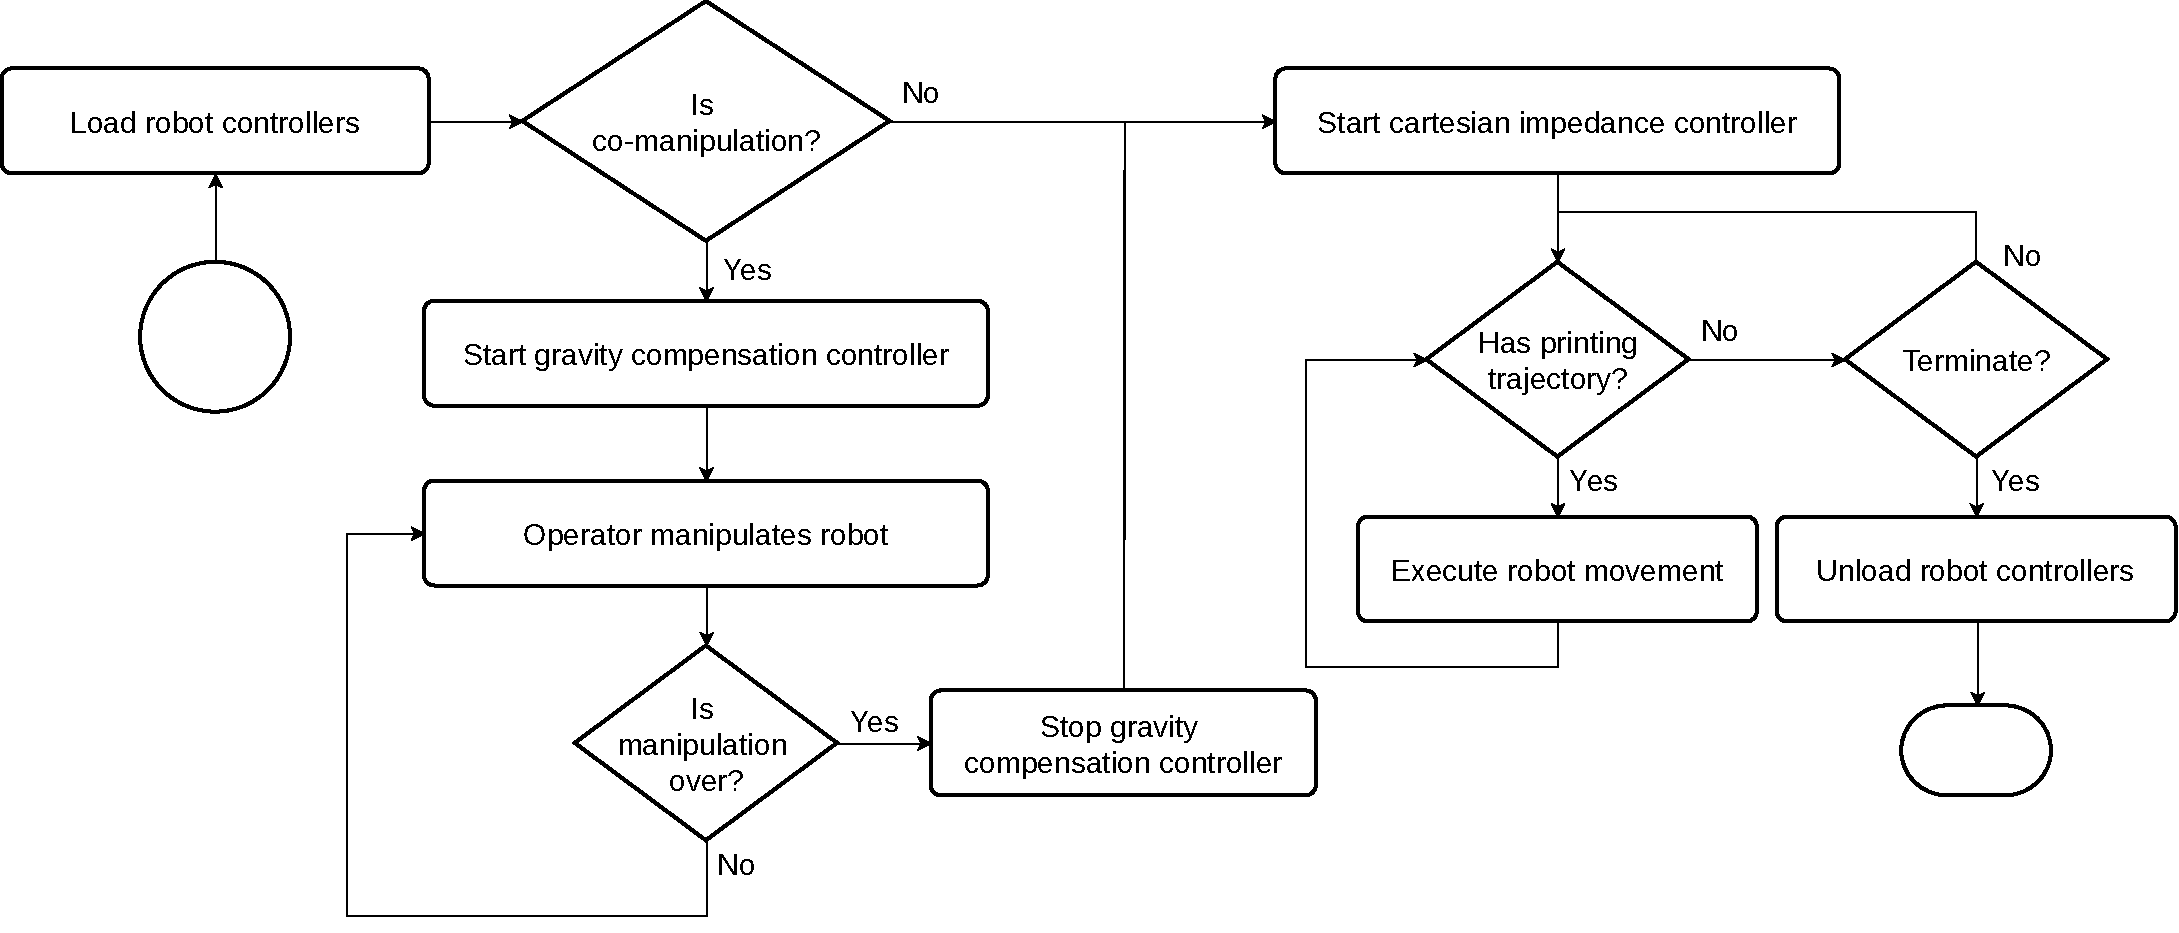
\includegraphics[width=\textwidth]{system_architecture_layer_robot_control_flowchart}
	\caption{Visual Servoing & Control layer flowchart. It is a general overview of the working of this layer.}
	\label{fig:system_architecture_layer_robot_control_flowchart}
\end{figure}

The control algorithms will be presented in detail on chapter \ref{cha:control_architectures}.

% subsubsection system_architectural_robot_layers_visual_servoing_control

% subsection system_architectural_robot_layers

\subsection{Print Head Layers}
\label{subsec:system_architectural_printhead_layers}

At the top of this layered architecture reside the print head layers. Their responsibility consists in controlling the bioink dispensing and monitor the available volume.

\subsubsection*{Bioink Management}
\label{subsubsec:system_architectural_printhead_layers_bioink_management}

The bottom layer is the bioink management layer. This layer monitors the available volume of bioink. When the bioink ends it sends information to the robot arm controller to stop the printing job and refill. Figure \ref{fig:system_architecture_layer_bioprint_bioink_management_flowchart} presents this layer flowchart.

\begin{figure}[htbp]
	\centering
	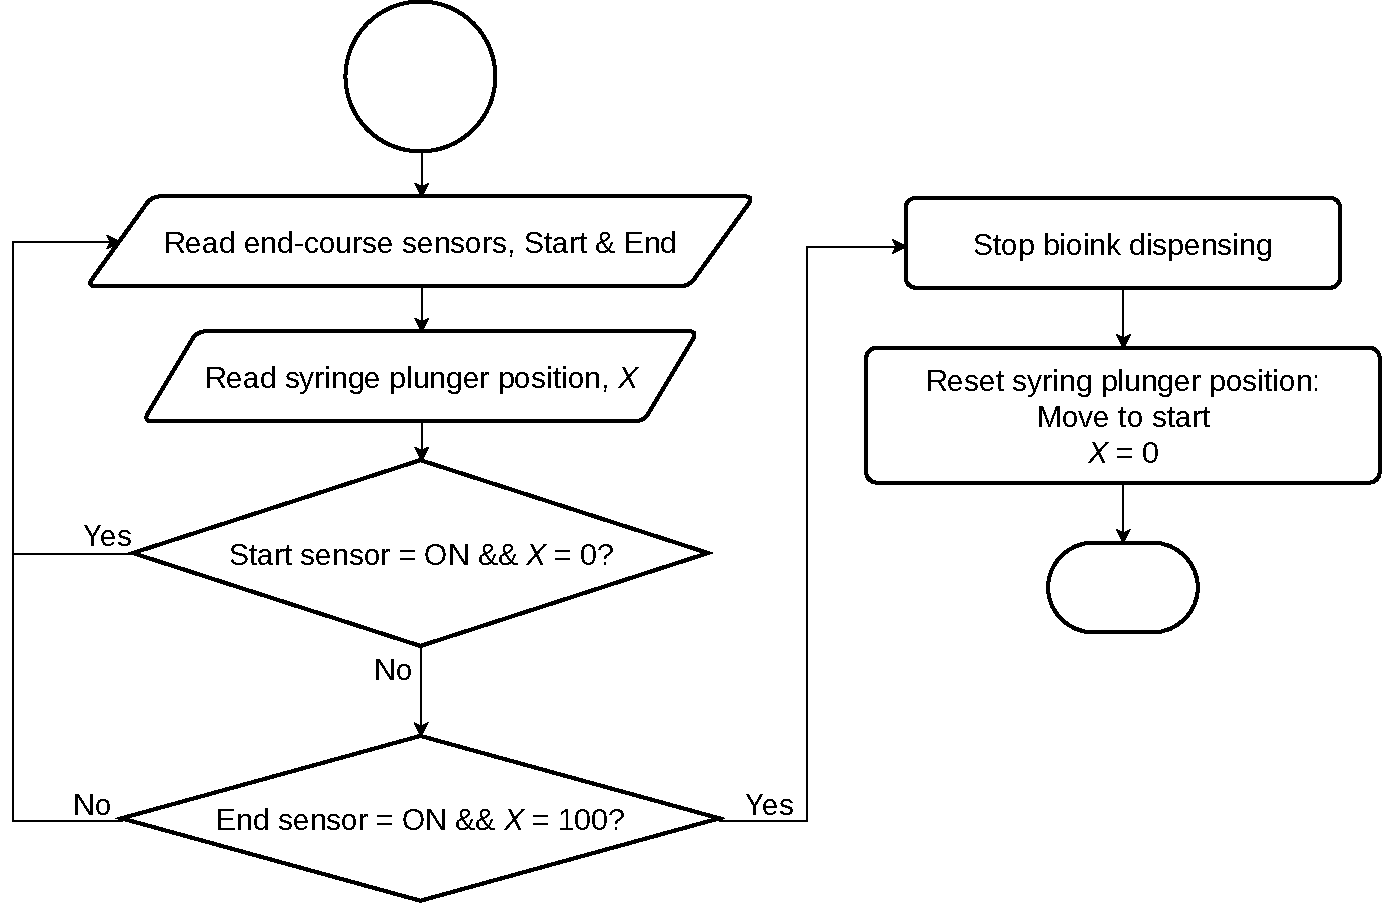
\includegraphics[width=\textwidth]{system_architecture_layer_bioprint_bioink_management_flowchart}
	\caption{Bioink management layer flowchart. The goal of this layer is to constantly monitor the bioink available volume by tracking the syringe plunger position. If the position reaches the end, the bioink dispensing is stopped and the position reset.}
	\label{fig:system_architecture_layer_bioprint_bioink_management_flowchart}
\end{figure}

The volume is tracked by measuring the syringe plunger position with time. This is accomplished via two hardware end of course switches and by tracking motor action. The switches are actuated when the plunger is at its limit positions. The motor action allows a precise position tracking because of the lead screw mechanism. 

More details on the mechanism are available on chapter \ref{cha:bioprinting_system}.

% subsubsection system_architectural_printhead_layers_bioink_management

\subsubsection*{Bioink Dispensing Control}
\label{subsubsec:system_architectural_printhead_layers_bioink_dispensing_control}

At the very top we have the bioink dispensing control layer. This layer is responsible for controlling when the bioink dispensing happens based on the bioprinting action commands received. Besides commanding the actions, this layer also controls the dispensing speed based on the printing speed. Figure \ref{fig:system_architecture_layer_bioprint_dispensing_control_flowchart} presents this layer flowchart.

\begin{figure}[htbp]
	\centering
	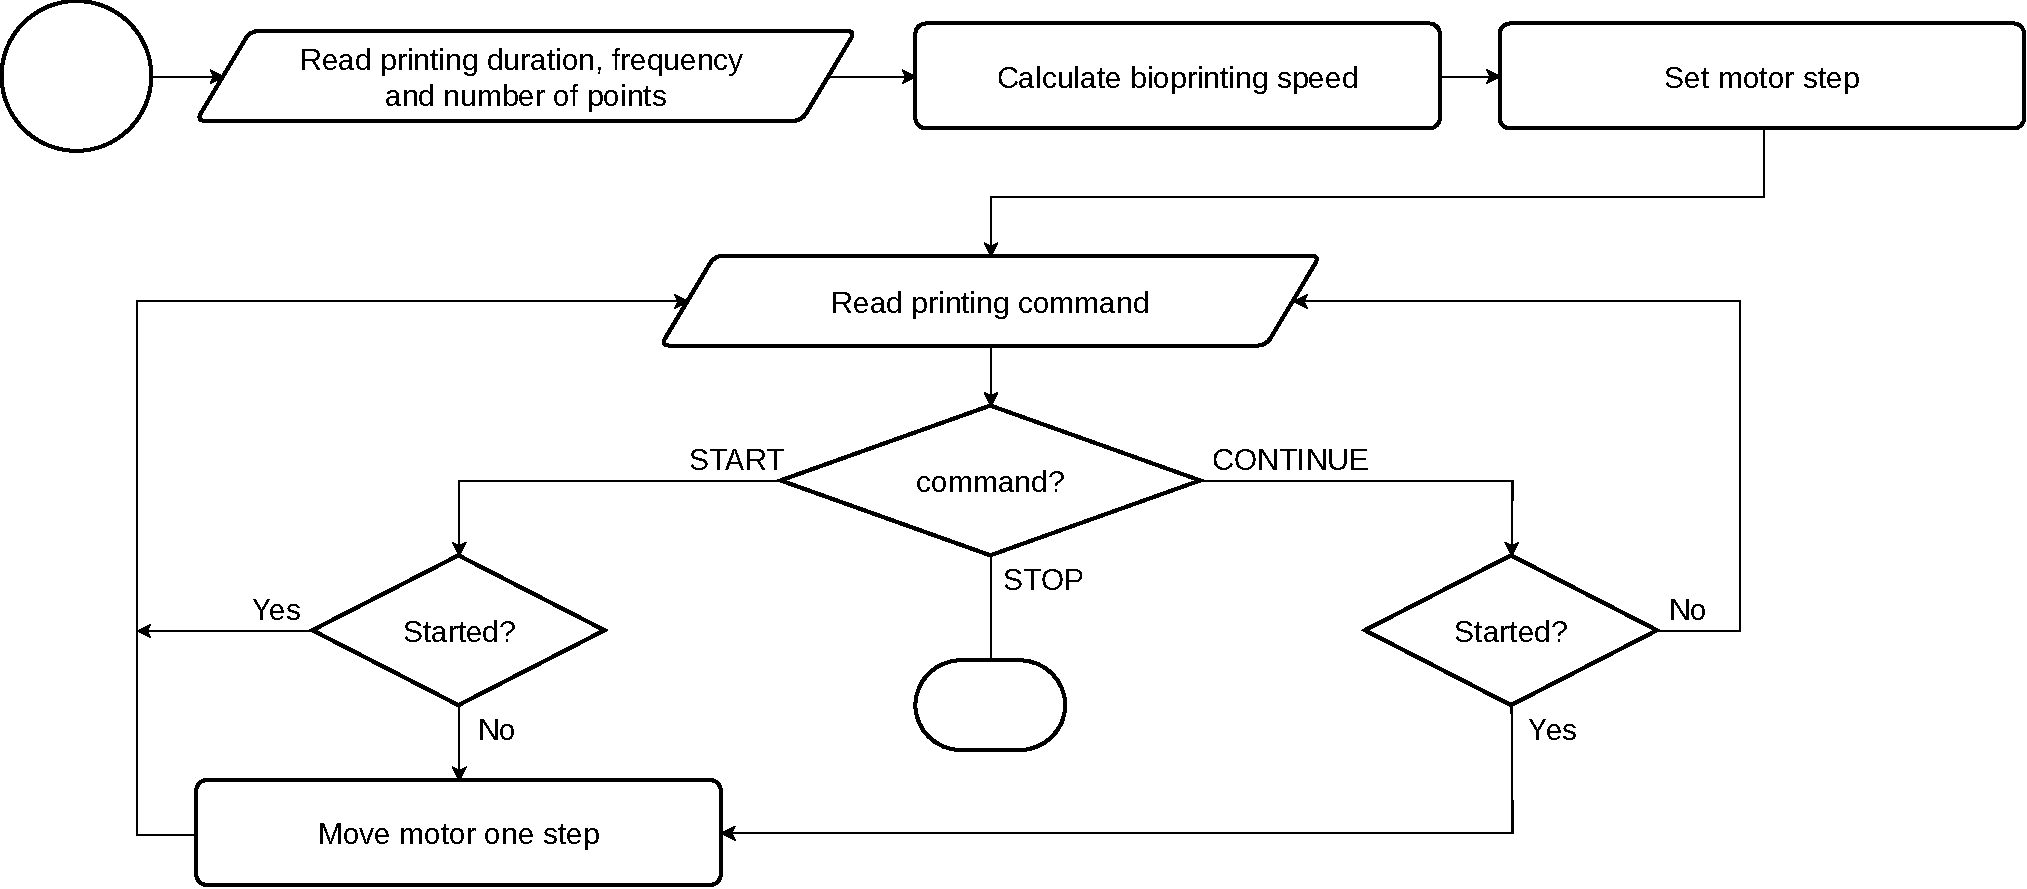
\includegraphics[width=\textwidth]{system_architecture_layer_bioprint_dispensing_control_flowchart}
	\caption{Bioink dispensing layer flowchart. It starts by calculating the motor step based on printing duration, control frequency and number of trajectory points. Afterwards, it moves the motor depending on the commands received.}
	\label{fig:system_architecture_layer_bioprint_dispensing_control_flowchart}
\end{figure}

More details on the mechanism are available on chapter \ref{cha:bioprinting_system}.

% subsubsection system_architectural_printhead_layers_bioink_dispensing_control

% subsection system_architectural_printhead_layers